% Created 2024-05-22 Τετ 14:18
% Intended LaTeX compiler: pdflatex
\documentclass[11pt]{report}
\usepackage[utf8]{inputenc}
\usepackage[T1]{fontenc}
\usepackage{graphicx}
\usepackage{longtable}
\usepackage{wrapfig}
\usepackage{rotating}
\usepackage[normalem]{ulem}
\usepackage{amsmath}
\usepackage{amssymb}
\usepackage{capt-of}
\usepackage{hyperref}
\usepackage{booktabs}
\usepackage{import}
\usepackage[LGR, T1]{fontenc}
\usepackage[greek, english, american]{babel}
\usepackage{alphabeta}
\usepackage{esint}
\usepackage{mathtools}
\usepackage{esdiff}
\usepackage{makeidx}
\usepackage[acronym]{glossaries}
\usepackage{newfloat}
\usepackage{minted}
\usepackage[a4paper, margin=3cm]{geometry}
\usepackage{chemfig}
\usepackage{svg}
\usepackage[automake]{glossaries-extra}
\usepackage{fancyhdr}
\geometry{a4paper,width=150mm,top=25mm,bottom=25mm}
\makeglossaries
\newcommand{\HRule}{\rule{\linewidth}{0.5mm}}
\date{}
\title{ΒΙΟΑΠΟΔΟΜΗΣΗ ΥΠΟΛΕΙΜΜΑΤΩΝ ΤΡΟΦΙΜΩΝ ΚΑΙ ΠΑΡΑΓΩΓΗ ΒΙΟΑΕΡΙΟΥ ΜΕΣΩ ΑΝΑΕΡΟΒΙΑΣ ΧΩΝΕΥΣΗΣ ΣΕ ΕΡΓΑΣΤΗΡΙΑΚΗ ΚΑΙ ΠΙΛΟΤΙΚΗ ΚΛΙΜΑΚΑ Προβλήματα στην αναερόβια χώνευση Μεθόδοι Επεξεργασίας Οξεογένεση Οξικογένεση και Μεθανογένεση Πειραματική Διαδικασία}
\hypersetup{
 pdfauthor={Βιδιάνος Γιαννίτσης},
 pdftitle={ΒΙΟΑΠΟΔΟΜΗΣΗ ΥΠΟΛΕΙΜΜΑΤΩΝ ΤΡΟΦΙΜΩΝ ΚΑΙ ΠΑΡΑΓΩΓΗ ΒΙΟΑΕΡΙΟΥ ΜΕΣΩ ΑΝΑΕΡΟΒΙΑΣ ΧΩΝΕΥΣΗΣ ΣΕ ΕΡΓΑΣΤΗΡΙΑΚΗ ΚΑΙ ΠΙΛΟΤΙΚΗ ΚΛΙΜΑΚΑ Προβλήματα στην αναερόβια χώνευση Μεθόδοι Επεξεργασίας Οξεογένεση Οξικογένεση και Μεθανογένεση Πειραματική Διαδικασία},
 pdfkeywords={},
 pdfsubject={},
 pdfcreator={Emacs 29.3 (Org mode 9.6.15)}, 
 pdflang={English}}
\makeatletter
\newcommand{\citeprocitem}[2]{\hyper@linkstart{cite}{citeproc_bib_item_#1}#2\hyper@linkend}
\makeatother

\usepackage[notquote]{hanging}
\begin{document}

\renewcommand{\abstractname}{Περίληψη}
\renewcommand{\tablename}{Πίνακας}
\renewcommand{\figurename}{Σχήμα}
\renewcommand{\chaptername}{Κεφάλαιο}
\renewcommand{\chapterautorefname}{Κεφάλαιο}
\renewcommand{\sectionautorefname}{Ενότητα}
\renewcommand{\partname}{Μέρος}
\renewcommand{\listfigurename}{Περιεχόμενα Σχημάτων: }
\renewcommand{\listtablename}{Περιεχόμενα Πινάκων: }
\renewcommand\listingscaption{Κώδικας}
\pagestyle{fancy}
\fancyhead{}
\fancyhead[L]{\chaptername~\thechapter}
\fancyhead[R]{Βιδιάνος Γιαννίτσης}
\newacronym{fw}{ΥΤ}{υπολείμματα τροφών}
\newacronym{fao}{FAO}{Οργανισμός Τροφίμων και Αγρονομίας των Ηνωμένων Πολιτειών}
\newacronym{co2eq}{$CO_2$-eq}{ισοδύναμο διοξειδίου του άνθρακα}
\newacronym{xyta}{ΧΥΤΑ}{Χώρους Υγειονομικής Ταφής Απορριμάτων}
\newacronym{syngas}{syngas}{αέριο σύνθεσης}
\newacronym{pla}{PLA}{πολυγαλακτικό οξύ}
\newacronym{trl}{TRL}{technology readiness level}
\newacronym{vfa}{VFAs}{πτητικά λιπαρά οξέα}
\newacronym{hrt}{HRT}{υδραυλικός χρόνος παραμονής}
\newacronym{olr}{OLR}{ρυθμός οργανικής φόρτισης}
\newacronym{uasb}{UASB}{αντιδραστήρας ανοδικής ροής διαμέσου στρώσης ιλύος}
\newacronym{mix}{μιξ}{σκεύασμα ενζύμων και μικροοργανισμών}
\newacronym{ad}{ΑΧ}{αναερόβια χώνευση}
\newacronym{ts}{TS}{ολικά στερεά}
\newacronym{vs}{VS}{πτητικά στερεά}
\newacronym{cod}{COD}{χημικά απαιτούμενο οξυγόνο}
\newacronym{scod}{sCOD}{διαλυτό COD}
\newacronym{tcod}{tCOD}{ολικό COD}
\newacronym{pi}{PI}{Process Intensification}
\newacronym{ssf}{SSF}{Solid State Fermentation}
\newacronym{orp}{ORP}{οξειδοαναγωγικό δυναμικό}
\newacronym{emp}{EMP}{μονοπάτι Embden-Meyerhof}
\newacronym{lcfa}{LCFA}{long chain fatty acids}
\newacronym{acet-coa}{Acetyl-CoA}{ακέτυλο συνένζυμο Α}
\newacronym{nad}{NAD$^+$}{nicotinamide adenine dinucleotide}
\newacronym{nadh}{NADH}{nicotinamide adenine dinucleotide hydrogen}
\newacronym{fd}{Fd}{ferredoxins}
\newacronym{dg}{ΔG}{μεταβολή ελεύθερης ενέργειας Gibbs}
\newacronym{abe}{ABE}{ζύμωση ακετόνης-βουτανόλης-αιθανόλης}
\newacronym{ed}{ED}{μονοπάτι Entner-Doudoroff}
\newacronym{pp}{PP}{μονοπάτι Pentose Phosphate}
\newacronym{pk}{PK}{μονοπάτι Phosphoketolase}
\newacronym{am}{AM}{ακετοκλαστικοί μεθανογόνοι}
\newacronym{hm}{YM}{υδρογονοτρόφοι μεθανογόνοι}
\newacronym{zvi}{ZVI}{σίδηρος μηδενικού σθένους}
\newacronym{redox}{redox}{οξειδωαναγογικό δυναμικό}
\newacronym{iht}{IHT}{interspecies hydrogen transfer}
\newacronym{diet}{DIET}{direct interspecies electron transfer}
\newacronym{tvfa}{tVFAs}{συνολικά πτητικά λιπαρά οξέα}
\newacronym{bmp}{BMP}{βιοχημικό δυναμικό μεθανίου}
\newacronym{sma}{SMA}{ειδική μεθανογόνος δραστικότητα της λάσπης}
\newacronym{kel}{ΚΕΛ}{κέντρο επεξεργασίας λυμάτων}
\newacronym{ss}{SS}{αιωρούμενα στερεά}
\newacronym{tss}{TSS}{ολικά αιωρούμενα στερεά}
\newacronym{vss}{VSS}{πτητικά αιωρούμενα στερεά}
\newacronym{hplc}{HPLC}{υγρή χρωματογραφία υψηλής απόδοσης}
\newacronym{si}{S/I}{υποστρώματος προς εμβόλιο}

\renewcommand{\contentsname}{Κεφάλαια: }
\begin{titlepage}

\begin{center}
  \begin{minipage}{0.2\textwidth}
    \begin{flushleft}
      \includegraphics[width=1\textwidth]{~/Pictures/ntua_logo.png}\\[0.4cm]    
    \end{flushleft}
  \end{minipage}
  \begin{minipage}{0.75\textwidth}
    \textsc{\bfseries \Large ΕΘΝΙΚΟ ΜΕΤΣΟΒΙΟ ΠΟΛΥΤΕΧΝΕΙΟ}\\[0.2cm]
    \textsc{\bfseries \Large ΣΧΟΛΗ ΧΗΜΙΚΩΝ ΜΗΧΑΝΙΚΩΝ}\\[0.2cm]
    \textsc{\large \bfseries ΤΟΜΕΑΣ IV: ΣΥΝΘΕΣΗ ΚΑΙ ΑΝΑΠΤΥΞΗ ΒΙΟΜΗΧΑΝΙΚΩΝ ΔΙΑΔΙΚΑΣΙΩΝ}\\[0.2cm]
    \textsc{\bfseries \large ΕΡΓΑΣΤΗΡΙΟ ΟΡΓΑΝΙΚΗΣ ΧΗΜΙΚΗΣ \\ ΤΕΧΝΟΛΟΓΙΑΣ}\\[0.2cm]
  \end{minipage}
  \\[2.5cm]

  \HRule \\[0.3cm]
  \Huge Βιοαποδόμηση Υπολειμμάτων Τροφίμων και Παραγωγή Βιοαερίου μέσω Αναερόβιας Χώνευσης σε Εργαστηριακή και Πιλοτική Κλίμακα\\[2.5cm]

  \huge Διπλωματική Εργασία \\[0.3cm]
   \begin{minipage}{0.4\textwidth}
    \begin{flushleft}
      \emph{\LARGE Συγγραφέας:}\\
	\emph{\LARGE Αριθμός Μητρώου:} \\
	\emph{\LARGE e-mail:}
      \end{flushleft}
    \end{minipage}
    \begin{minipage}{0.4\textwidth}
      \begin{flushright} \large
	\LARGE Βιδιάνος Γιαννίτσης\\
	\LARGE ch19113\\
	\LARGE vidianosgiannitsis@gmail.com
      \end{flushright}
    \end{minipage}
    \HRule \\[0.3cm]
  \vfill
{\LARGE Αθήνα, 2024}

\end{center}

\end{titlepage}

\part*{Περιεχόμενα}
\label{sec:org93a9519}
\tableofcontents
\pagebreak

\listoffigures
\pagebreak

\listoftables
\pagebreak

\printglossary
\printglossary[type = \acronymtype, title = Συντομογραφίες]

\part{Θεωρητικό Μέρος}
\label{sec:orgc464ed1}
\chapter{Εισαγωγή}
\label{sec:org1c3dd5c}

Τα \acrfull{fw} αποτελούν ένα σημαντικό πρόβλημα στις σύγχρονες κοινωνίες. Ο \acrfull{fao} υπολογίζει πως περίπου το 1/3 της παγκόσμιας παραγωγής τροφών ετησίως (1.3 δις τόνοι) χάνεται κατά την παραγωγική διαδικασία ή απορρίπτεται (\citeprocitem{29}{Ishangulyyev, Kim, and Lee 2019}).

Η μη ορθή διαχείριση των αποβλήτων αυτών επιβαρύνει κάθε έναν από τους τρεις πυλώνες της βιωσιμότητας. Συγκεκριμένα, έχει προσδιοριστεί πως το \acrfull{co2eq} που παράγεται λόγω της μη ορθής αυτής διαχείρισης των υπολειμμάτων ανέρχεται στους 3.3 δις τόνους (\citeprocitem{72}{Taheri et al. 2021}) . Ακόμη, έχει βρεθεί πως τα υπολείμματα τροφών που οφείλονται μόνο στην απόρριψη τροφών από καταναλωτές σε ανεπτυγμένες χώρες είναι σχεδόν όσα παράγουν οι υπό σαχάριες και αφρικανικές χώρες συνολικά (περίπου 230 εκατομμύρια) (\citeprocitem{29}{Ishangulyyev, Kim, and Lee 2019}). Οπότε η αποφυγή της δημιουργίας τόσων υπολειμμάτων - ή η καλύτερη αξιοποίηση τους - θα μπορούσε να λύσει πολλά προβλήματα υποσιτισμού. Ακόμη και στον οικονομικό τομέα, δημιουργούνται σοβαρά προβλήματα από την ανεξέλεγκτη αυτή απόρριψη καθώς η καθαρή αξία των τροφών που χάνονται ή απορρίπτονται σε κάποιο σημείο της εφοδιαστικής αλυσίδας είναι 936 δις δολάρια ανά έτος με ελάχιστο κέρδος, καθώς πολύ μικρές ποσότητες των υπολειμμάτων αυτών αξιοποιούνται (\citeprocitem{29}{Ishangulyyev, Kim, and Lee 2019}) .

Μία από τις βασικότερες υποκατηγορίες \acrshort{fw} είναι τα οικιακά \acrshort{fw}, τα οποία αποτελούν το μεγαλύτερο κομμάτι της παγκόσμιας παραγωγής \acrshort{fw} (περίπου \(61 \%\)) (\citeprocitem{68}{“Statista - The Statistics Portal” 2023}) . Στο \figurename \ref{fig:org2b7537b} φαίνεται η παγκόσμια παραγωγή \acrshort{fw} ανά τομέα.
\begin{figure}[htbp]
\centering
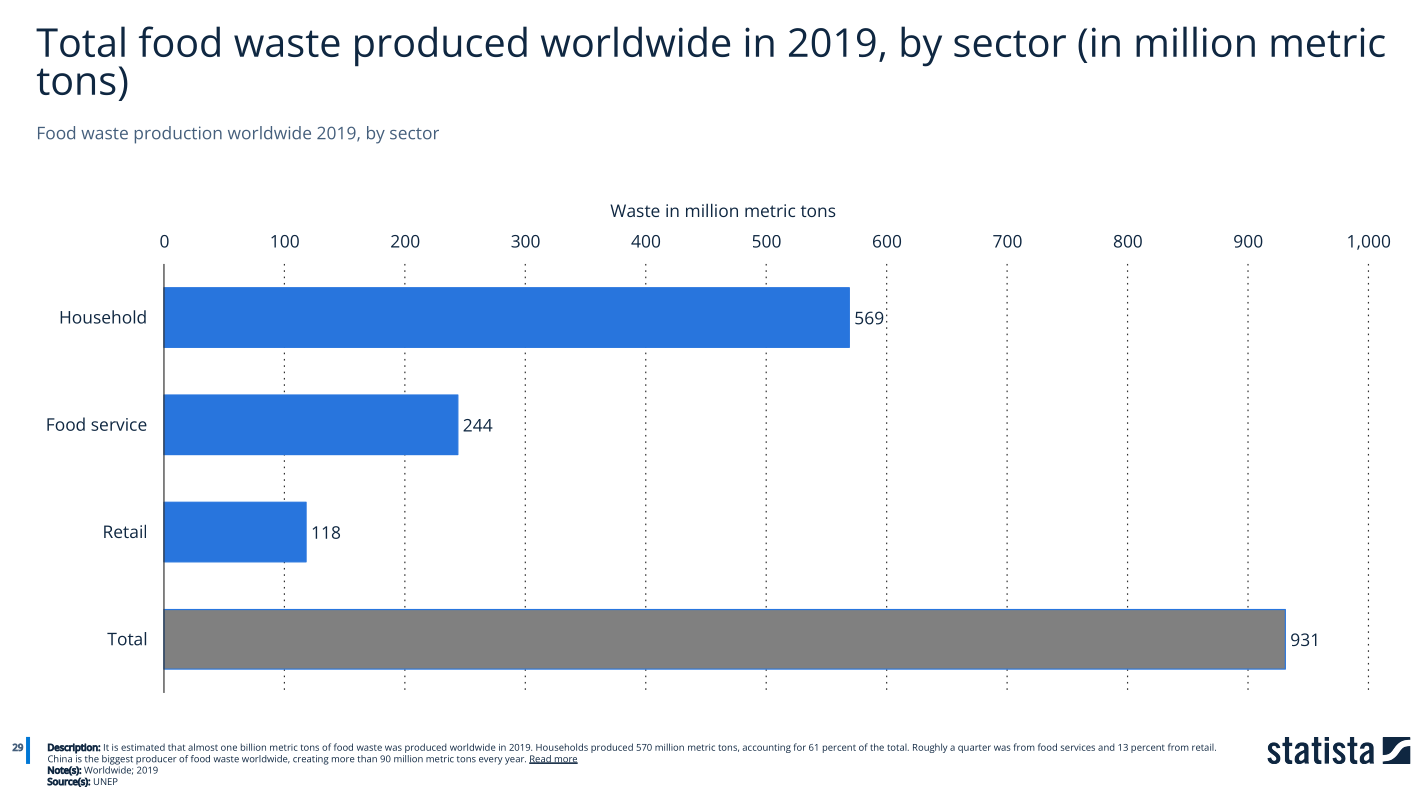
\includegraphics[width=300px]{../plots/statistics/statistic_food_waste_by_sector_2019.png}
\caption{\label{fig:org2b7537b}Παγκόσμια παραγωγή υπολειμμάτων τροφών ανά τομέα}
\end{figure}

Η Ελλάδα είναι η χώρα με την δεύτερη μεγαλύτερη παραγωγή οικιακών \acrshort{fw} κατά κεφαλήν παγκοσμίως (142 κιλά/άτομο ετησίως) (\citeprocitem{68}{“Statista - The Statistics Portal” 2023}) . Η παραγωγή \acrshort{fw}, ειδικά στον τομέα της κατανάλωσης, όπου βρίσκονται τα οικιακά υπολείμματα, καθώς και αυτά της εστίασης, είναι πολύ συχνά αναπόφευκτη. Οπότε, παρόλο που με πιο σωστές πρακτικές θα μπορούσαν να παράγονται λιγότερα υπολείμματα, η ανάπτυξη τεχνολογιών αξιοποίησης των \acrshort{fw} είναι πάρα πολύ σημαντικές. Οι τεχνολογίες αυτές θα πρέπει να είναι εύκολα εφαρμόσιμες και οικονομικές, ενώ η κλιμάκωση τους να είναι εφικτή.

Η αγορά της διαχείρισης αποβλήτων είναι αρκετά μεγάλη (υπολογίζεται περίπου στα 1293 δις δολάρια ετησίως από μία μελέτη του 2022), ενώ προβλέψεις λένε πως θα φτάσει τα 2000 δις μέχρι το 2030. Κομμάτι της ανάπτυξης αυτής, θα πρέπει να είναι και η ανάπτυξη βιώσιμων τεχνολογιών αξιοποίησης απορριμμάτων, καθώς αυτή την στιγμή, με εξαίρεση τα απορρίμματα τα οποία είναι ανακυκλώσιμα, οι βασικές τεχνολογίες που εφαρμόζονται είναι η ανάκτηση ενέργειας μέσω καύσης και η διάθεση των απορριμμάτων σε \acrfull{xyta} όπως φαίνεται και στο \figurename  \ref{fig:org617ddbe} (\citeprocitem{68}{“Statista - The Statistics Portal” 2023}).

\begin{figure}[htbp]
\centering
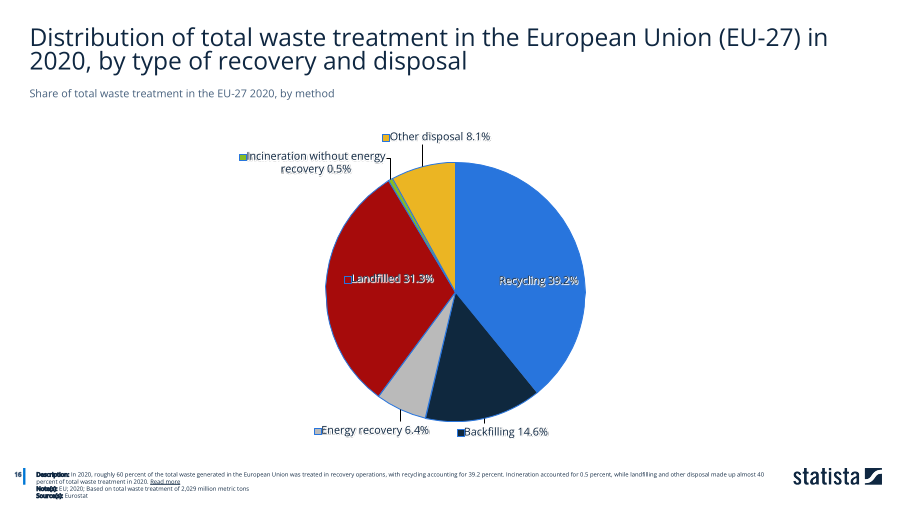
\includegraphics[width=.9\linewidth]{../plots/statistics/statistic_waste_treatment_technologies_europe_2020.png}
\caption{\label{fig:org617ddbe}Τεχνολογίες επεξεργασίας απορριμμάτων στην Ευρωπαική Ένωση}
\end{figure}

Οι τεχνολογίες αυτές χρησιμοποιούνται επειδή είναι πολύ απλές και έχουν χαμηλό κόστος. Στα πλαίσια όμως της βιώσιμης ανάπτυξης και της κυκλικής οικονομίας, πρέπει τα απορρίμματα να εξετάζονται ως μία νέα πρώτη ύλη, από την οποία μπορούν να διυλιστούν προϊόντα αυξημένης αξίας.

Αυτές οι τεχνολογίες μπορεί να είναι θερμικές, όπως η πυρόλυση (\citeprocitem{51}{Pardo et al. 2023}; \citeprocitem{78}{Usmani et al. 2021}) η οποία παράγει ένα προϊόν γνωστό ως biochar, το οποίο έχει πολύ χρήσιμες ιδιότητες (\citeprocitem{88}{Xu et al. 2024}; \citeprocitem{28}{Infurna, Caruso, and Dintcheva 2023}), ή η αεριοποίηση (\citeprocitem{78}{Usmani et al. 2021}; \citeprocitem{48}{Murugesan et al. 2022}), η οποία παράγει ένα μίγμα υδρογόνου και μονοξειδίου του άνθρακα γνωστό ως \acrfull{syngas}, το οποίο μπορεί να χρησιμοποιηθεί ως πρώτη ύλη για πολλά προϊόντα. Στο \figurename  \ref{fig:org9ae93dd} φαίνονται κάποια κλασσικά παραδείγματα αυτού (\citeprocitem{77}{Udaeta et al. 2007})

\begin{figure}[htbp]
\centering
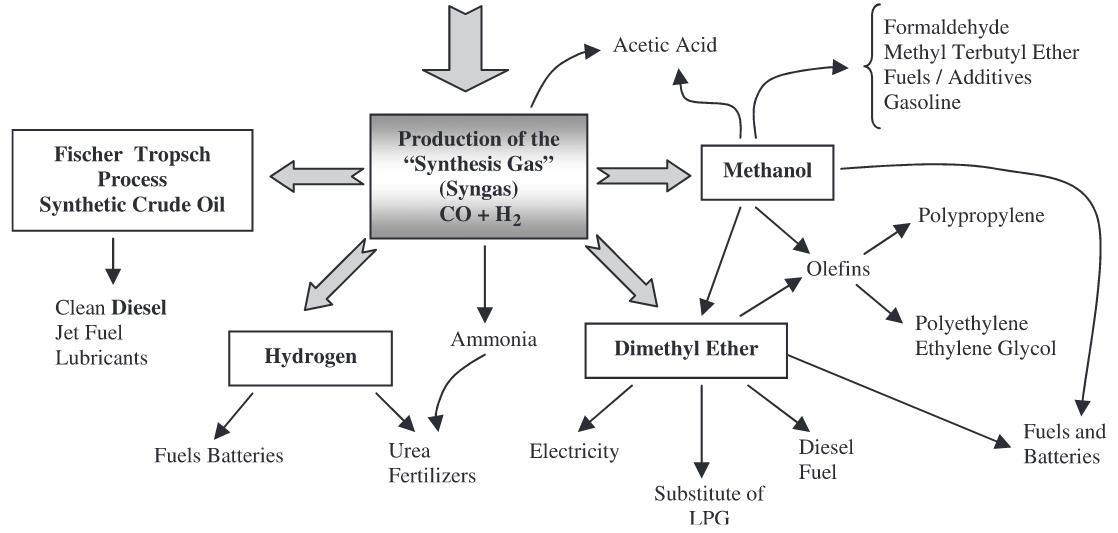
\includegraphics[width=.9\linewidth]{./gasification_products.jpg}
\caption[Προιόντα του αερίου σύνθεσης]{\label{fig:org9ae93dd}Προιόντα του αερίου σύνθεσης (\citeprocitem{77}{Udaeta et al. 2007})}
\end{figure}

Εκτός από θερμικές τεχνολογίες, υπάρχει μεγάλο ενδιαφέρον στις βιολογικές τεχνολογίες. Αυτές μπορεί να είναι αερόβιες, όπως η κομποστοποίηση, η οποία παράγει ένα εδαφοβελτιωτικό προϊόν (\citeprocitem{9}{Cerda et al. 2018}), ή αναερόβιες όπως η αναερόβια χώνευση, η οποία έχει ως κύριο προϊόν το βιοαέριο, ένα μείγμα μεθανίου και διοξειδίου του άνθρακα που μπορεί να χρησιμοποιηθεί ως βιοκαύσιμο (\citeprocitem{42}{Ma et al. 2018}; \citeprocitem{87}{Xu et al. 2018}), ή διάφορες διεργασίες ζύμωσης. Σε αυτές υπάγονται η αλκοολική ζύμωση, μία από τις πιο ευρέως χρησιμοποιούμενες τεχνολογίες αξιοποίησης απορριμμάτων (\citeprocitem{1}{Anwar Saeed et al. 2018}; \citeprocitem{61}{Roukas and Kotzekidou 2022}), η σκοτεινή ζύμωση για την παραγωγή υδρογόνου (\citeprocitem{90}{Yasin et al. 2013}; \citeprocitem{44}{Mohanakrishna et al. 2023}), ή οι ζυμώσεις με σκοπό την παραγωγή μονομερών για βιοπολυμερή όπως το \acrfull{pla} (\citeprocitem{57}{Rajesh Banu and Godvin Sharmila 2023}; \citeprocitem{54}{Pleissner et al. 2017}) .

Η παρούσα μελέτη θα εστιάσει στην \acrfull{ad}, καθώς είναι μία τεχνολογία με μεγάλο δείκτη ετοιμότητας \acrfull{trl} (\citeprocitem{43}{Mankins 1995}), η οποία έχει εφαρμοστεί επιτυχώς σε μεγάλη κλίμακα, είναι οικονομική και φιλική προς το περιβάλλον (\citeprocitem{23}{Franchetti 2013}) .

Η \acrshort{ad} είναι μία αναερόβια βιολογική διεργασία η οποία διακρίνεται σε 4 στάδια. Στο πρώτο στάδιο, το αρχικό υπόστρωμα της διεργασίας, το οποίο συχνά αποτελείται από περίπλοκα πολυμερή όπως οι υδατάνθρακες, οι πρωτεΐνες και τα λιπίδια, υδρολύονται σε απλούστερες ενώσεις. Αυτές μπορούν να χρησιμοποιηθούν από τα οξεογόνα βακτήρια τα οποία τα μετατρέπουν σε \acrfull{vfa} όπως το οξικό οξύ, το προπιονικό οξύ, το βουτυρικό οξύ ή το γαλακτικό οξύ και σε αλκοόλες όπως η αιθανόλη. Στο 3ο στάδιο, οι ενώσεις αυτές μετατρέπονται σε οξικό οξύ, υδρογόνο και διοξείδιο του άνθρακα κατά την διεργασία της οξικογένεσης, ενώ τελικά, το οξικό οξύ μετατρέπεται σε μεθάνιο από μία κατηγορία μεθανογόνων μικροοργανισμών ενώ το υδρογόνο και το διοξείδιο του άνθρακα μετατρέπονται σε μεθάνιο από μία άλλη κατηγορία μεθανογόνων. Τα στάδια αυτά φαίνονται και στο \figurename \ref{fig:org3e2c71a} (\citeprocitem{25}{Grippi, Clemente, and Bernal 2020}) .

\begin{figure}[htbp]
\centering
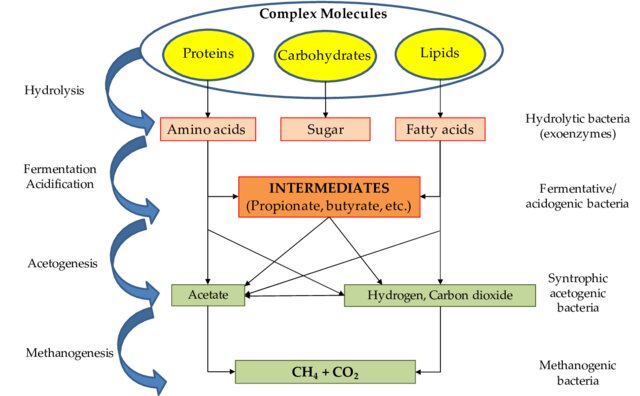
\includegraphics[width=280px]{./anaerobic_digestion_phases.jpg}
\caption[Φάσεις της αναερόβιας χώνευσης]{\label{fig:org3e2c71a}Φάσεις της αναερόβιας χώνευσης (\citeprocitem{25}{Grippi, Clemente, and Bernal 2020})}
\end{figure}

Ακόμη, είναι μία πολύ καλή τεχνολογία για την αξιοποίηση των \acrshort{fw} καθώς είναι πλούσια σε οργανική ύλη, η οποία είναι εύκολα αποδομήσιμη αλλά και σε θρεπτικά στοιχεία όπως το άζωτο, με υψηλότερο C/N από πολλά υποστρώματα. Λόγω αυτών, μπορούν να μετατραπούν πολύ αποτελεσματικά σε βιοαέριο (\citeprocitem{42}{Ma et al. 2018}).

Επιπροσθέτως, η \acrshort{ad} λύνει και άλλο ένα από τα σημαντικά προβλήματα του 21ου αιώνα, το οποίο είναι η ενέργεια. Αυτή τη στιγμή, πάνω από το \(80 \%\) της ενέργειας που καταναλώνεται παγκοσμίως βασίζεται σε μη ανανεώσιμες πηγές όπως το πετρέλαιο και το φυσικό αέριο. Οι ενεργειακές απαιτήσεις παγκοσμίως έχουν μία συνεχή αύξηση, ενώ οι πρώτες ύλες αυτές εξαλείφονται (\citeprocitem{68}{“Statista - The Statistics Portal” 2023}) . Οπότε, τεχνολογίες παραγωγής ενέργειας από ανανεώσιμες πηγές, οι οποίες να έχουν το δυναμικό να αντικαταστήσουν τις πηγές αυτές, θα γίνουν απαραίτητες τα επόμενα χρόνια. Οι περισσότερες τεχνολογίες ανανεώσιμης ενέργειας (πχ αιολική, ηλιακή ή υδροηλεκτρική ενέργεια) έχουν δυσκολία να φτάσουν τέτοια επίπεδα και για αυτό χρησιμοποιούνται επικουρικά σε μία κύρια πηγή ενέργειας (αυτή τη στιγμή, περίπου το \(30 \%\) της παγκόσμιας παραγωγής ηλεκτρισμού οφείλεται σε τέτοιες πηγές) (\citeprocitem{68}{“Statista - The Statistics Portal” 2023}) . Τα υπολείμματα τροφών από την άλλη είναι άφθονα οπότε θεωρείται πως με μία αποτελεσματική επεξεργασία θα μπορέσουν να καλύψουν ένα πολύ σημαντικό ποσοστό της παγκόσμιας ανάγκης σε ενέργεια.

Στο \figurename \ref{fig:org259349a} φαίνεται η παγκόσμια παραγωγή ενέργειας από βιοαέριο τα τελευταία 15 χρόνια, η οποία έχει ραγδαία αύξηση (\citeprocitem{68}{“Statista - The Statistics Portal” 2023}) .

\begin{figure}[htbp]
\centering
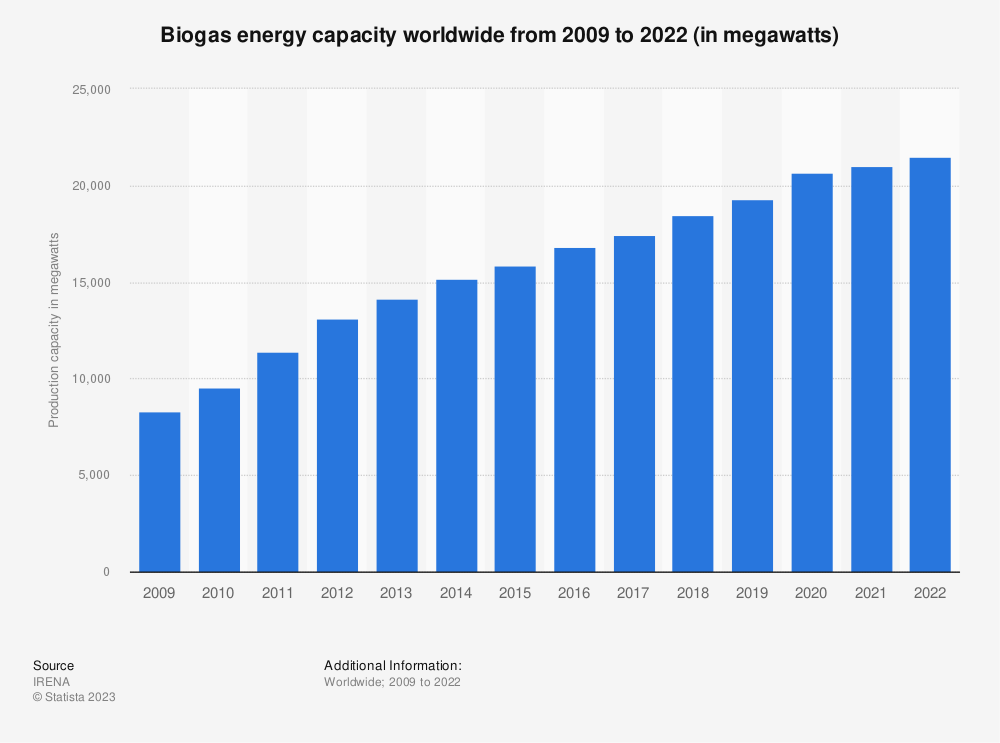
\includegraphics[width=.9\linewidth]{../plots/statistics/statistic_id1032922_global-biogas-energy-capacity-2009-2022.png}
\caption{\label{fig:org259349a}Παγκόσμια παραγωγή ενέργειας από βιοαέριο}
\end{figure}

Βέβαια, η \acrshort{ad} έχει και κάποια σημαντικά προβλήματα. Ο βασικός περιορισμός της είναι η ευαισθησία των μεθανογόνων μικροοργανισμών στις περιβαλλοντικές συνθήκες. Λόγω της ευαισθησίας τους, η \acrshort{ad} λειτουργεί στις βέλτιστες συνθήκες αυτών. Αυτό όμως οδηγεί στην λιγότερο αποτελεσματική διεξαγωγή των άλλων σταδίων. Το κυριότερο πρόβλημα που δημιουργείται είναι πως η υδρόλυση μπορεί μεν να διεξαχθεί, αλλά γίνεται σε πολύ αργό ρυθμό, καθιστώντας την το περιοριστικό στάδιο της \acrshort{ad} και τον λόγο για τον οποίο θεωρείται μία αρκετά αργή διεργασία. Ένα αντίστοιχο πρόβλημα υπάρχει και στο στάδιο της οξεογένεσης, όπου οι μικροοργανισμοί δεν λειτουργούν στις βέλτιστες συνθήκες τους και μπορούν να ακολουθήσουν μόνο ένα μεταβολικό μονοπάτι, το οποίο ενεργοποιείται στις συνθήκες που λειτουργούν. Έτσι, η οξεογένεση είναι πιθανόν να μην είναι ιδιαίτερα αποδοτική. Παρόλα αυτά, σε ορισμένες περιπτώσεις, ο ρυθμός της οξεογένεσης ξεπερνάει αυτόν της μεθανογένεσης (ο οποίος είναι γενικά αργός), με αποτέλεσμα να παράγονται υπερβολικές ποσότητες από \acrshort{vfa}, το οποίο οδηγεί σε οξίνιση του αντιδραστήρα και κατάρρευση της διεργασίας καθώς οι μεθανογόνοι δεν μπορούν να λειτουργήσουν σε εκείνες τις τιμές pH (\citeprocitem{78}{Usmani et al. 2021}; \citeprocitem{4}{Azbar, Ursillo, and Speece 2001}; \citeprocitem{105}{Zoetemeyer et al. 1982}).

Ένας τρόπος να επιλυθεί το πρόβλημα αυτό είναι ο διαχωρισμός των σταδίων της υδρόλυσης και της ζύμωσης, σε μία διεργασία δύο (\citeprocitem{55}{Pohland and Ghosh 1971}) ή τριών (\citeprocitem{96}{Zhang et al. 2017}) σταδίων. Αυτό που πετυχαίνεται με τον διαχωρισμό αυτόν είναι να λειτουργούν όλα τα στάδια της διεργασίας στο βέλτιστο σημείο λειτουργίας τους και άρα να είναι πολύ πιο αποτελεσματικά. Επιπροσθέτως, ο αντιδραστήρας δεν οξινίζεται κατά την διάρκεια της μεθανογένεσης, με αποτέλεσμα η διεργασία να είναι πολύ πιο σταθερή. Όμως, υπάρχει το πρόβλημα πως οι διεργασίες αυτές έχουν υψηλότερο κόστος, λόγω του περισσότερου εξοπλισμού, αλλά και πολυπλοκότητας της διεργασίας. Για τον λόγο αυτόν, η διεργασία αναερόβιας χώνευσης πολλαπλών σταδίων έχει πολύ χαμηλότερο \acrshort{trl} και δεν έχει εφαρμοστεί ευρέως σε μεγάλη κλίμακα (\citeprocitem{4}{Azbar, Ursillo, and Speece 2001}; \citeprocitem{82}{Wu et al. 2022}; \citeprocitem{42}{Ma et al. 2018}; \citeprocitem{78}{Usmani et al. 2021}) .

Η υδρόλυση αποτελεί σημαντικό στάδιο της επεξεργασίας \acrshort{fw}, καθώς έχουν υψηλή περιεκτικότητα σε βιοπολυμερή. Αυτή μπορεί να γίνει θερμικά, μηχανικά, χημικά ή ενζυμικά (\citeprocitem{67}{Srisowmeya, Chakravarthy, and Nandhini Devi 2020}; \citeprocitem{33}{Kavitha et al. 2017}; \citeprocitem{42}{Ma et al. 2018}). Συνήθως η υδρόλυση γίνεται ενζυμικά καθώς έχει καταγραφεί πως επιφέρει τις υψηλότερες αποδόσεις και δεν παράγει προϊόντα τοξικά για τους μικροοργανισμούς. Ακόμη, είναι η μόνη που μπορεί να γίνει παράλληλα με την οξεογένεση για την περίπτωση της αναερόβιας χώνευσης σε 2 στάδια (\citeprocitem{94}{Zhang et al. 2020}; \citeprocitem{26}{Han et al. 2016}; \citeprocitem{42}{Ma et al. 2018}) . Παρόλα αυτά, το υψηλό κόστος των ενζυμικών σκευασμάτων καθιστά αυτή την τεχνολογία απαγορευτική σε μεγάλη κλίμακα. Για αυτό, υπάρχει αρκετή έρευνα γύρω από τεχνολογίες μείωσης του κόστους της ενζυμικής υδρόλυσης για την πιο αποτελεσματική λειτουργία της διεργασίας αυτής (\citeprocitem{106}{Zou et al. 2020}; \citeprocitem{75}{Uçkun Kiran, Trzcinski, and Liu 2015}; \citeprocitem{64}{dos Santos Ferreira et al. 2020}; \citeprocitem{54}{Pleissner et al. 2017}). Μια υποσχόμενη και οικονομική λύση είναι η χρήση σκευασμάτων τα οποία περιέχουν ένζυμα αλλά και μικροοργανισμούς. Αυτά τα σκευάσματα επιτρέπουν την αποτελεσματική υδρόλυση των \acrshort{fw} αλλά ταυτόχρονα και μία ζύμωση για παραγωγή χρήσιμων προϊόντων, όπως η αιθανόλη και τα \acrshort{vfa}. Αυτά μπορούν να ανακτηθούν ως έχουν, ή να χρησιμοποιηθούν σε διάφορες βιοδιεργασίες, όπως η \acrshort{ad}. Ένα τέτοιο υπόστρωμα μπορεί να βελτιώσει την σταθερότητα μίας αναερόβιας χώνευσης αφού περιορίζονται τα στάδια της υδρόλυσης και οξεογένεσης και ευνοείται η δράση των μεθανογόνων μικροοργανισμών (\citeprocitem{78}{Usmani et al. 2021}).

Ο σκοπός της παρούσας μελέτης είναι αρχικά να κάνει μία βιβλιογραφική ανασκόπηση των τεχνολογιών \acrshort{ad} σε πολλαπλά στάδια. Με βάση αυτήν θα αναπτυχθεί μία διεργασία αξιοποίησης υπολειμμάτων τροφών, αξιοποιώντας ένα \acrfull{mix}, η οποία να είναι οικονομικά βιώσιμη αλλά ταυτόχρονα αποτελεσματική. Αρχικά, θα αξιολογηθεί η ποιότητα της υδρόλυσης καθώς και της οξεογένεσης κατά την διεργασία αυτή σε εργαστηριακή κλίμακα, όπου υπάρχει καλός έλεγχος παραμέτρων όπως η θερμοκρασία και η ποσότητα του \acrshort{mix}. Έπειτα, θα εξεταστεί η κλιμάκωση της διεργασίας σε πιλοτική κλίμακα εξετάζοντας την ποσότητα του \acrshort{mix} και την παροχή νερού ως λειτουργικές παραμέτρους. Τέλος, θα διερευνηθεί η δυνατότητα αξιοποίησης της παραγόμενης υγρής εκροής για την παραγωγή μεθανίου σε αναερόβιους αντιδραστήρες εργαστηριακής κλίμακας.

Η δομή της εργασίας θα είναι ως εξής: Στην συνέχεια του πρώτου μέρους θα γίνει η βιβλιογραφική ανασκόπηση, η οποία θα χωριστεί σε 5 κεφάλαια. Αρχικά, στο \autoref{sec:anaerobic_digestion} θα γίνει μία πιο αναλυτική παρουσίαση της \acrshort{ad} και των προβλημάτων που δημιουργούνται αν όλα τα στάδια αυτής γίνονται ταυτόχρονα. Σκοπός αυτού είναι η ανάδειξη της σημασίας της \acrshort{ad} σε πολλαπλά στάδια. Έτσι, τα επόμενα κεφάλαια θα εστιάσουν στα στάδια της \acrshort{ad} αν αυτά διεξαχθούν ξεχωριστά. Στο \autoref{sec:fw_pretreatment} θα αναλυθούν όλες οι μέθοδοι προ-επεξεργασίας υπολειμμάτων τροφών που έχουν βρεθεί στην βιβλιογραφία για να υδρολύσουν πιο αποτελεσματικά τα \acrshort{fw}, με τα πλεονεκτήματα και τα μειονεκτήματα τους, ενώ στο \autoref{sec:enzymes} θα δοθεί ιδιαίτερη έμφαση στην ενζυμική υδρόλυση, και στις προσπάθειες μείωσης του κόστους αυτής. Το \autoref{sec:acidogenesis} θα εστιάσει στην οξεογένεση και θα αναφέρει όλα τα διαθέσιμα μεταβολικά μονοπάτια αυτής και πως καθορίζεται ποιο θα επικρατήσει με βάση τις λειτουργικές συνθήκες. Ακόμη, θα αναφερθεί η χρησιμότητα του κάθε μεταβολικού προϊόντος για την \acrshort{ad} για να αποφανθεί το βέλτιστο μονοπάτι. Τέλος, στο \autoref{sec:methanogenesis} θα μελετηθούν η οξικογένεση και η μεθανογένεση. Τα 2 αυτά στάδια δεν θα διαχωριστούν, καθώς στην πράξη, το ένα εξαρτάται από το άλλο και γίνονται συνεργιστικά.

Έχοντας τις πληροφορίες αυτές, μπορεί στο δεύτερο μέρος, να γίνει μία ανάλυση των πειραματικών αποτελεσμάτων της εργασίας και να προκύψουν κάποια συμπεράσματα από αυτά. Συγκεκριμένα, στο \autoref{sec:materials_methods} θα αναλυθούν οι πειραματικές διαδικασίες που χρησιμοποιήθηκαν καθώς και οι πρώτες ύλες που χρειάστηκαν. Στο \autoref{sec:result_analysis} θα αναφερθεί τι αποτελέσματα είχε ο κάθε πειραματικός κύκλος και πως αυτά αναλύθηκαν με σκοπό στο \autoref{sec:result_discussion} να γίνει η παράθεση των τελικών αποτελεσμάτων κάθε κύκλου και μία συζήτηση αυτών. Έτσι θα προκύψουν κάποια συμπεράσματα καθώς και προτάσεις για περαιτέρω έρευνα στο αντικείμενο αυτό, τα οποία θα παρατεθούν στο \autoref{sec:conclusion}.

\chapter{Αναερόβια Χώνευση}
\label{sec:org20a9b3f}
\label{sec:anaerobic_digestion}

Η αναερόβια χώνευση είναι μία αναερόβια βιολογική διεργασία η οποία μετατρέπει περίπλοκη οργανική ύλη σε μεθάνιο και διοξείδιο του άνθρακα με βάση τον μηχανισμό του σχήματος \ref{fig:org3e2c71a}. Η διεργασία αυτή έχει πολλά πλεονεκτήματα, όπως η απλότητα της λειτουργίας, το χαμηλό σχετικά λειτουργικό κόστος (χρειάζεται μόνο η διατήρηση της θερμοκρασίας σε ένα σταθερό επίπεδο) και την παραγωγή ενός πολύ αποτελεσματικού ενεργειακού φορέα, του μεθανίου (\citeprocitem{67}{Srisowmeya, Chakravarthy, and Nandhini Devi 2020}). Για αυτούς τους λόγους μάλιστα έχει δει ραγδαία ανάπτυξη τα τελευταία χρόνια (\citeprocitem{68}{“Statista - The Statistics Portal” 2023}) .

Όμως, παραμένει περιορισμένη σε μεγάλο βαθμό από τα λειτουργικά της προβλήματα (\citeprocitem{67}{Srisowmeya, Chakravarthy, and Nandhini Devi 2020}). Αρχικά, είναι μία αργή διεργασία. Αυτό οφείλεται εν μέρει στους μεθανογόνους μικροοργανισμούς, οι οποίοι θέλουν ο \acrfull{hrt} να είναι μεγάλος για να μπορέσουν να αναπτυχθούν και να μην εκπλυθούν. Αλλά, για τα περισσότερα υποστρώματα, το περιοριστικό στάδιο της διεργασίας είναι η υδρόλυση και διαλυτοποίηση, δηλαδή η διάσπαση των στερεών και μακρομερών σωματιδίων σε διαλυτές ενώσεις, οι οποίες μπορούν να μεταβολιστούν. Στην περίπτωση των υπολειμμάτων τροφών, ένα μεγάλο ποσό της οργανικής ύλης βρίσκεται σε σωματιδιακή μορφή και δεν είναι διαλυτό. Είναι στην πλειοψηφία του ένα εύκολα υδρολύσιμο υπόστρωμα, αλλά αν η υδρόλυση γίνει κατά την διάρκεια της χώνευσης, επιβραδύνει τον χρόνο που διαρκεί η χώνευση (\citeprocitem{33}{Kavitha et al. 2017}; \citeprocitem{42}{Ma et al. 2018}; \citeprocitem{78}{Usmani et al. 2021}) . Αυτό γίνεται επειδή κατά την λειτουργία ενός χωνευτήρα, οι λειτουργικές συνθήκες ρυθμίζονται στις βέλτιστες των μεθανογόνων μικροοργανισμών, οι οποίοι είναι οι πιο ευαίσθητοι. Αυτές είναι συνήθως στη μεσόφιλη περιοχή της θερμοκρασίας (35-37 \(^oC\)) και σε pH κοντά στο ουδέτερο (6.4-8.0). Αντιθέτως, η βέλτιστη λειτουργία της υδρόλυσης από τους ήδη υπάρχοντες μικροοργανισμούς στην λάσπη είναι βέλτιστη σε πολύ πιο όξινα pH (\citeprocitem{97}{Zhang et al. 2019}; \citeprocitem{96}{Zhang et al. 2017}) και τα συνήθη υδρολυτικά ένζυμα που εκκρίνονται από τους μικροοργανισμούς αυτούς λειτουργούν βέλτιστα σε υψηλότερες θερμοκρασίες (\citeprocitem{42}{Ma et al. 2018}; \citeprocitem{94}{Zhang et al. 2020}; \citeprocitem{8}{Cekmecelioglu and Uncu 2013}) . Για τους λόγους αυτούς, είναι συχνό να γίνεται κάποια προ-επεξεργασία πριν την αναερόβια χώνευση, η οποία αποσκοπεί στην υδρόλυση και διαλυτοποίηση του υποστρώματος (\citeprocitem{10}{Cesaro and Belgiorno 2014}; \citeprocitem{24}{Graunke and Wilkie 2014}; \citeprocitem{67}{Srisowmeya, Chakravarthy, and Nandhini Devi 2020}; \citeprocitem{42}{Ma et al. 2018}) .

Το άλλο βασικό πρόβλημα της αναερόβιας χώνευσης, είναι η ανισορροπία στους ρυθμούς της αντίδρασης. Στην περίπτωση που και τα 4 στάδια γίνονται ταυτόχρονα, μία ευσταθής συνθήκη λειτουργίας, θα ήταν όλα τα στάδια να έχουν τον ίδιο ρυθμό, ώστε ότι παράγεται να καταναλώνεται. Στην πράξη όμως, αυτό δεν συμβαίνει. Οι οξεογόνοι μικροοργανισμοί συχνά μεταβολίζουν το υπόστρωμα τους πιο γρήγορα από τους μεθανογόνους, οπότε σε πολλές περιπτώσεις μπορεί να παρατηρηθεί συσσώρευση πτητικών λιπαρών οξέων. Η συσσώρευση αυτή σημαίνει πως θα μειωθεί το pH του αντιδραστήρα σε ένα επίπεδο που θα ανασχεθεί η λειτουργία των μεθανογόνων μικροοργανισμών και σταδιακά θα σταματήσει η παραγωγή μεθανίου, κάτι που θα συντελέσει στην κατάρρευση του συστήματος. Η ανισορροπία αυτή στους ρυθμούς μπορεί όμως να συντελέσει και άλλο ένα πρόβλημα. Εκτός από \acrshort{vfa}, παράγεται και υδρογόνο κατά την οξεογένεση. Η υψηλή μερική πίεση υδρογόνου στο σύστημα είναι επίσης ανασχετική για τους μεθανογόνους και μπορεί να οδηγήσει το σύστημα σε κατάρρευση. Λόγω των προβλημάτων αυτών, το σύστημα αναερόβιας χώνευσης ενός σταδίου, δεν έχει ιδιαίτερα μεγάλη σταθερότητα (\citeprocitem{67}{Srisowmeya, Chakravarthy, and Nandhini Devi 2020}; \citeprocitem{87}{Xu et al. 2018}; \citeprocitem{4}{Azbar, Ursillo, and Speece 2001}; \citeprocitem{96}{Zhang et al. 2017}) .

Ο συμβατικός τρόπος που επιλύεται αυτό είναι o χαμηλός \acrfull{olr}. Αν το σύστημα τροφοδοτείται με μικρή ποσότητα υποστρώματος, θα είναι χαμηλός γενικά ο ρυθμός της οξεογένεσης, με αποτέλεσμα να είναι πιο δύσκολο να δημιουργηθεί αστάθεια. Βέβαια, η χρήση πολύ χαμηλού \acrshort{olr} είναι προβληματική επειδή περιορίζει σημαντικά τον ρυθμό επεξεργασίας του αποβλήτου. Ειδικά στην περίπτωση των υπολειμμάτων τροφών τα οποία παράγονται σε πολύ μεγάλους ρυθμούς, θα ήταν ιδανικό ο χωνευτήρας να λειτουργεί σε υψηλό ρυθμό οργανικής φόρτισης. Ένας τρόπος να αυξηθεί ο \acrshort{olr} είναι η χρήση ενός ταχύρυθμου αντιδραστήρα όπως ο \acrfull{uasb}. Στον αντιδραστήρα αυτόν, η λάσπη που δημιουργείται είναι κοκκώδης και παρατηρείται σχηματισμός βιοφίλμ. Έτσι, ο κάθε κόκκος αποτελεί ένα μικροβιακό οικοσύστημα όπου οι πιο ευαίσθητοι μικροοργανισμοί, όπως οι μεθανογόνοι προστατεύονται από τις εξωτερικές συνθήκες. Αυτό έχει ως αποτέλεσμα η διεργασία να έχει μεγαλύτερη σταθερότητα και να μπορεί να διεξαχθεί πιο γρήγορα. Αυτό επιτρέπει και την αύξηση του \acrshort{olr} (\citeprocitem{4}{Azbar, Ursillo, and Speece 2001}; \citeprocitem{82}{Wu et al. 2022}; \citeprocitem{84}{Wu et al. 2016}) .

Όμως, ο πιο αποτελεσματικός τρόπος να αυξηθεί ο \acrlong{olr} σε έναν αντιδραστήρα αναερόβιας χώνευσης είναι μία διάταξη σε δύο στάδια (\citeprocitem{55}{Pohland and Ghosh 1971}; \citeprocitem{105}{Zoetemeyer et al. 1982}; \citeprocitem{4}{Azbar, Ursillo, and Speece 2001}). Σε αυτή, διαχωρίζονται τα στάδια της υδρόλυσης και οξεογένεσης από την μεθανογένεση. Ως αποτέλεσμα, η εκροή του οξεογενή αντιδραστήρα μπορεί να υποστεί μία ρύθμιση pH στην περιοχή που λειτουργούν βέλτιστα οι μεθανογόνοι και εφόσον έχει ολοκληρωθεί ήδη η οξεογένεση, δεν υπάρχει ο κίνδυνος να οξινιστεί ο αντιδραστήρας, κάτι που θα οδηγούσε στην κατάρρευση του. Έτσι, τα συστήματα αυτά είναι πολύ πιο σταθερά και μπορούν να λειτουργήσουν σε μεγαλύτερα \acrshort{olr} πολύ αποτελεσματικά (\citeprocitem{55}{Pohland and Ghosh 1971}; \citeprocitem{82}{Wu et al. 2022}). Ακόμη ένα πλεονέκτημα της διάταξης αυτής είναι πως διαχωρίζοντας τα στάδια της υδρόλυσης και της οξεογένεσης, το οποίο επιτρέπει την λειτουργία τους σε πιο επιθυμητές συνθήκες. Η οξεογένεση είναι μία περίπλοκη διεργασία η οποία μπορεί να ακολουθήσει πολλά μεταβολικά μονοπάτια ανάλογα με τις συνθήκες στις οποίες θα διεξαχθεί. Η επιλογή του βέλτιστου μονοπατιού εξαρτάται από πολλούς παράγοντες και θα αναλυθεί περαιτέρω στο \autoref{sec:acidogenesis}, αλλά είναι κάτι που είναι εφικτό μόνο σε συστήματα δύο φάσεων. Η βέλτιστη λειτουργία της υδρόλυσης είναι λίγο πιο καθορισμένη. Όμως, συνήθως δεν λαμβάνεται υπόψιν στα συστήματα δύο φάσεων, καθώς συνήθως καθορίζονται από την οξεογένεση. Καθώς η υδρόλυση λειτουργεί βέλτιστα σε όξινα pH, η λειτουργία της στο σύστημα αυτό είναι σίγουρα πιο αποτελεσματική από την υδρόλυση στο σύστημα μίας φάσης (\citeprocitem{82}{Wu et al. 2022}; \citeprocitem{42}{Ma et al. 2018}; \citeprocitem{4}{Azbar, Ursillo, and Speece 2001}; \citeprocitem{78}{Usmani et al. 2021}). Στην βιβλιογραφία, υπάρχουν και κάποια συστήματα αναερόβιας χώνευσης τριών σταδίων (\citeprocitem{78}{Usmani et al. 2021}; \citeprocitem{97}{Zhang et al. 2019}; \citeprocitem{96}{Zhang et al. 2017}; \citeprocitem{35}{Kim and Kim 2013}), στα οποία λειτουργεί και η υδρόλυση ξεχωριστά και στο βέλτιστο σημείο λειτουργίας της. Η διεργασία αυτή είναι πιο αποτελεσματική και πιο σταθερή, αλλά ταυτόχρονη ακόμη πιο περίπλοκη. Οπότε, γενικά προτιμάται η διεργασία δύο σταδίων, ως μία ισορροπία μεταξύ πολυπλοκότητας και σταθερότητας της λειτουργίας (\citeprocitem{78}{Usmani et al. 2021}).

\chapter{Προεπεξεργασία Υπολειμμάτων Τροφών}
\label{sec:org908a93e}
\label{sec:fw_pretreatment}

Τα \acrshort{fw} έχουν υψηλή περιεκτικότητα σε βιοπολυμερή. Για να μπορέσουν να χρησιμοποιηθούν αποδοτικά ως ένα υπόστρωμα για διεργασίες όπως η \acrshort{ad}, απαιτείται κάποια διεργασία η οποία θα υδρολύσει το υπόστρωμα αυτό. Υπάρχουν πολλές τεχνολογίες για να βοηθήσουν την υδρόλυση του υποστρώματος αυτού όπως η μηχανική, θερμική, χημική ή ενζυμική προεπεξεργασία και η προ-επεξεργασίες με υπερήχους και μικροκύματα.

\section{Μηχανική Επεξεργασία}
\label{sec:org121665e}
Η πιο απλή είναι η μηχανική επεξεργασία. Μία μηχανική επεξεργασία όπως ο τεμαχισμός είναι αρκετά αποτελεσματική. Ο σκοπός της είναι η ομογενοποίηση της στερεής μάζας και μείωση του μεγέθους κόκκων της ώστε να επιταχυνθούν τα επόμενα στάδια της προ-επεξεργασίας. Είναι το πιο σύνηθες στάδιο προ-επεξεργασίας και γίνεται ανεξαρτήτως των επόμενων σταδίων συνήθως (\citeprocitem{13}{Chen et al. 2022}; \citeprocitem{45}{Moon and Song 2011}; \citeprocitem{78}{Usmani et al. 2021}) . 

\section{Θερμική Επεξεργασία}
\label{sec:org1cc01dd}
Η θερμική υδρόλυση βασίζεται στην αύξηση της θερμοκρασίας, με σκοπό την διάσπαση των πολυμερικών δεσμών. Είναι πολύ αποτελεσματική ως μία προ-επεξεργασία για δύσκολα αποδομήσιμη βιομάζα. Στην περίπτωση των \acrshort{fw}, οι υψηλές θερμοκρασίες δεν είναι αναγκαίες για την αποικοδόμηση και μάλιστα συνήθως υποβαθμίζουν την ποιότητα του υποστρώματος καθώς καταστρέφουν οργανική ύλη και μπορεί να παράξουν προϊόντα θερμικής αποδόμησης τα οποία είναι τοξικά για επόμενα βιολογικά στάδια. Ακόμη, είναι μία τεχνική με σχετικά υψηλές ενεργειακές απαιτήσεις (\citeprocitem{67}{Srisowmeya, Chakravarthy, and Nandhini Devi 2020}; \citeprocitem{10}{Cesaro and Belgiorno 2014}; \citeprocitem{42}{Ma et al. 2018}) .

\section{Επεξεργασία με Μικροκύματα}
\label{sec:org300d446}
Αντίστοιχη λογική έχει και η χρήση μικροκυμάτων, η οποία αυξάνει την θερμοκρασία μέσω ενός ηλεκτρομαγνητικού πεδίου. Θεωρείται πιο αποτελεσματική από την θερμική τεχνολογία λόγω της μικρότερης κατανάλωσης ενέργειας. Επίσης, συνδυάζει θερμικά με μη θερμικά φαινόμενα. Όμως, όπως και στη περίπτωση της θερμικής υδρόλυσης, δεν επιφέρει ιδιαίτερα θετικά αποτελέσματα για την επεξεργασία \acrshort{fw} (\citeprocitem{10}{Cesaro and Belgiorno 2014}; \citeprocitem{42}{Ma et al. 2018}; \citeprocitem{67}{Srisowmeya, Chakravarthy, and Nandhini Devi 2020}) . 

\section{Επεξεργασία με Υπερήχους}
\label{sec:org06a6b27}
Η χρήση υπερήχων βασίζεται στην δημιουργία ελεύθερων ριζών υδροξυλίου \(OH^{\cdot}\), οι οποίες διασπούν ταχύτατα τα στερεά, απελευθερώνοντας μεγάλα ποσά οργανικής ύλης. Πειράματα που έχουν χρησιμοποιήσει υπερήχους ως μία προ-επεξεργασία για αναερόβια χώνευση έχουν δείξει πως βελτιώνει αρκετά την παραγωγή μεθανίου. Βέβαια, υδρολύουν μόνο σε περιορισμένο βαθμό το υπόστρωμα, με αποτέλεσμα να πρέπει να γίνει και κάποια υδρόλυση κατά την διάρκεια της χώνευσης (\citeprocitem{10}{Cesaro and Belgiorno 2014}; \citeprocitem{42}{Ma et al. 2018}) .

\section{Χημική Επεξεργασία}
\label{sec:org8e65b76}
Σε ένα παρόμοιο μηχανισμό βασίζεται και η χημική τεχνολογία της οζόνωσης, καθώς η τροφοδοσία με όζον δημιουργεί και αυτή ελεύθερες ρίζες οι οποίες διασπούν την στερεή οργανική ύλη. Είναι όμως μία πιο έντονη επεξεργασία η οποία χρησιμοποιείται σε υποστρώματα τα οποία είναι πιο δύσκολα στην αποδόμηση. Στην περίπτωση των \acrshort{fw} μπορεί να οδηγήσουν σε μείωση του COD λόγω οξείδωσης ακόμη και των ζυμώσιμων σακχάρων και παραγωγής προϊόντων πιο δύσκολα αποδομήσιμα από τα αρχικά, για αυτό αποφεύγεται (\citeprocitem{67}{Srisowmeya, Chakravarthy, and Nandhini Devi 2020}; \citeprocitem{10}{Cesaro and Belgiorno 2014}) .

Βέβαια, η πιο συχνή κατηγορία χημικής επεξεργασίας είναι αυτή που βασίζεται στην προσθήκη οξέος ή βάσης. Η προσθήκη των ενώσεων αυτών βασίζεται στην επίτευξη ακραίων τιμών pH, στις οποίες καταρρέει η πολυμερική δομή. Στην τεχνολογία αυτή χρησιμοποιούνται ισχυρά οξέα ή βάσεις (πχ θειικό οξύ, υδροχλωρικό οξύ, καυστικό νάτριο ή ασβέστης). Η τεχνολογία αυτή είναι η πιο απλή και φθηνή τεχνολογία προ-επεξεργασίας, αλλά είναι και αρκετά αποτελεσματική. Για αυτό χρησιμοποιείται αρκετά (\citeprocitem{10}{Cesaro and Belgiorno 2014}; \citeprocitem{42}{Ma et al. 2018}; \citeprocitem{94}{Zhang et al. 2020}). Ακόμη, για την αλκαλική υδρόλυση, ισχύει πως αν τα \acrshort{fw} χρησιμοποιηθούν μετά για αναερόβια χώνευση, το σύστημα θα έχει αποκτήσει μεγαλύτερη αλκαλικότητα, με αποτέλεσμα να έχει καλύτερη σταθερότητα η διεργασία (\citeprocitem{67}{Srisowmeya, Chakravarthy, and Nandhini Devi 2020}) . Όμως, μπορεί να παραχθούν μη επιθυμητά προϊόντα κατά την όξινη ή αλκαλική αποδόμηση των \acrshort{fw}, όπως η φουρφουράλη, τα οποία είναι τοξικά προς μικροοργανισμούς και άρα να μειωθεί σημαντικά η απόδοση της διεργασίας (\citeprocitem{26}{Han et al. 2016}; \citeprocitem{94}{Zhang et al. 2020}; \citeprocitem{42}{Ma et al. 2018}) .

\section{Ενζυμική Επεξεργασία}
\label{sec:org938432d}
Τέλος, υπάρχει η ενζυμική επεξεργασία. Αυτή βασίζεται στην χρήση υδρολυτικών ενζύμων όπως οι υδατανθρακάσες, οι πρωτεάσες και οι λιπάσες για την διάσπαση των βιοπολυμερών. Η διεργασία αυτή δεν έχει κανένα τοξικό παραπροϊόν, ήπιες συνθήκες (οι οποίες συνδέονται με το κόστος) και εξαιρετική απόδοση υδρόλυσης/βιοαποδόμησης (\citeprocitem{42}{Ma et al. 2018}; \citeprocitem{26}{Han et al. 2016}; \citeprocitem{32}{Jing et al. 2020}). Επίσης, είναι η μόνη προ-επεξεργασία, της οποίας οι συνθήκες μπορούν να ρυθμιστούν έτσι ώστε να γίνει ταυτόχρονα με την οξεογένεση, το οποίο επιτρέπει την αναερόβια χώνευση σε 2 στάδια. Σε κάθε άλλη περίπτωση, η διεργασία πρέπει να γίνει σε τρία στάδια, το οποίο παρότι προσφέρει σταθερότητα και πιθανόν καλύτερες αποδόσεις, δημιουργεί και πολυπλοκότητα στην διεργασία (\citeprocitem{78}{Usmani et al. 2021}; \citeprocitem{42}{Ma et al. 2018}) . Παρόλα αυτά, το κόστος ενός εμπορικού ενζυμικού σκευάσματος είναι πολύ υψηλό, κάτι που καθιστά την συμβατική ενζυμική υδρόλυση μία τεχνολογία απαγορευτική σε μεγάλη κλίμακα. Για τον λόγο αυτόν, στην βιβλιογραφία υπάρχουν αρκετές μελέτες χρησιμοποιώντας πρωτοποριακές τεχνολογίες ενζυμικής υδρόλυσης χαμηλού κόστους για να λύσουν το πρόβλημα αυτό (\citeprocitem{12}{Chen et al. 2020}; \citeprocitem{96}{Zhang et al. 2017}; \citeprocitem{64}{dos Santos Ferreira et al. 2020}; \citeprocitem{54}{Pleissner et al. 2017}; \citeprocitem{71}{Suresh et al. 2020}) . Οι τεχνολογίες αυτές θα αναλυθούν σε περισσότερο βάθος στο \autoref{sec:enzymes}.

\section{Απόκριση της Υδρόλυσης}
\label{sec:org6dde0c0}
Αλλά μία σημαντική ερώτηση που έγκειται για την υδρόλυση, είναι πως προσδιορίζεται πειραματικά η απόδοση μίας τέτοιας διεργασίας. Στην πράξη, το σημαντικότερο μέτρο για αυτό είναι ο λόγος \acrfull{scod} προς \acrfull{tcod}. Αυτό δείχνει πόση από την οργανική ύλη έχει διαλυτοποιηθεί και στα \acrshort{fw} ξεκινάει από \(20-30 \%\) συνήθως και μπορεί να φτάσει από \(60 - 80 \%\) σε μία αρκετά αποδοτική υδρόλυση (\citeprocitem{33}{Kavitha et al. 2017}; \citeprocitem{24}{Graunke and Wilkie 2014}; \citeprocitem{20}{Fang et al. 2020}) .

\chapter{Βελτιστοποίηση της Διεργασίας της Ενζυμικής Υδρόλυσης}
\label{sec:orga28da50}
\label{sec:enzymes}

Στο \autoref{sec:fw_pretreatment} αναφέρθηκαν όλες οι τεχνολογίες προ-επεξεργασίας των \acrshort{fw}. Σκοπός αυτών είναι η επίτευξη υψηλών αποδόσεων σε επόμενα βιολογικά στάδια όπως η \acrshort{ad}. Προέκυψε, πως η ενζυμική υδρόλυση/βιοαποδόμηση είναι η πιο αποτελεσματική καθώς δεν έχει παραπροϊόντα, χρησιμοποιεί ήπιες συνθήκες, μειώνει αποτελεσματικά τα \acrfull{ts} και αυξάνει το διαλυτό \acrfull{cod}, ενώ μπορεί να γίνει παράλληλα με την οξεογένεση. Όμως, αναφέρθηκε πως το κύριο εμπόδιο της είναι το κόστος των ενζυμικών σκευασμάτων. Για αυτό, στο κεφάλαιο αυτό θα αναφερθούν όλες οι τεχνολογίες που έχουν προταθεί στην βιβλιογραφία για την μείωση του κόστους της διεργασίας αυτής. Γενικά, κατατάσσονται σε δύο κατηγορίες:

\begin{itemize}
\item Εντατικοποίηση της διεργασίας υδρόλυσης (\acrfull{pi}) και μείωση του απαιτούμενου χρόνου υδρόλυσης, ο οποίος σε συνεχή συστήματα αντιστοιχεί στην ποσότητα ενζύμων που απαιτούνται.
\item Χρήση μικροοργανισμών, οι οποίοι στις κατάλληλες συνθήκες θα εκκρίνουν υδρολυτικά ένζυμα in-situ για την υδρόλυση
\end{itemize}

\section{Εντατικοποίηση της Διεργασίας Υδρόλυσης}
\label{sec:org51941a5}
Οι μελέτες οι οποίες υπάγονται σε αυτήν την κατηγορία αποτελούν τις μελέτες οι οποίες έχουν προσπαθήσει να βελτιστοποιήσουν διάφορες συνθήκες της υδρόλυσης, με σκοπό την πιο αποτελεσματική και γρήγορη ενζυμική υδρόλυση, η οποία θα έχει χαμηλότερο κόστος.

Για παράδειγμα, οι (\citeprocitem{24}{Graunke and Wilkie 2014}) προσπάθησαν να μειώσουν πολύ τον χρόνο παραμονής στην υδρόλυση και έδειξαν ότι με βέλτιστες συνθήκες, σε περίπου 4 ώρες έχει γίνει ικανοποιητική υδρόλυση. Καθώς ο χρόνος αυτός συχνά είναι στις 24 ώρες, μία τέτοια μείωση θα μπορούσε να μειώσει σημαντικά την απαίτηση σε ένζυμα και άρα να βελτιώσει το οικονομικό προφίλ της διεργασίας (\citeprocitem{46}{Moon et al. 2009}; \citeprocitem{42}{Ma et al. 2018}; \citeprocitem{95}{Zhang, Ling, and Huo 2021}) .

Οι (\citeprocitem{71}{Suresh et al. 2020}) έκαναν μία μελέτη στην οποία προσπάθησαν να βελτιστοποιήσουν μία διεργασία παραγωγής βιοαιθανόλης από απόβλητα της βιομηχανίας επεξεργασίας πατάτας λαμβάνοντας υπόψιν συνθήκες όπως η ποσότητα ενζύμων που θα χρησιμοποιηθεί και η πιθανότητα χρήσης άλλων διεργασιών υδρόλυσης επικουρικά, όπως η προσθήκη HCl ή χρήση υπερήχων κατά την διεργασία.

Οι (\citeprocitem{41}{Li et al. 2019}) χρησιμοποίησαν έναν συνδυασμό υπερήχων και ενζυμικής υδρόλυσης με σκοπό οι υπέρηχοι να κάνουν την βιομάζα πιο προσβάσιμη στα ένζυμα, με σκοπό να μειωθεί σημαντικά η ποσότητα ενζύμων που πρέπει να προστεθεί. Η μελέτη τους έδειξε πως αυτός ο συνδυασμός είναι αρκετά αποτελεσματικός.

Παρόλο που υπήρχαν αρκετές επιτυχίες στον τομέα αυτόν, ακόμη και με σημαντική μείωση της ποσότητας ενζύμων που χρειάζονται, όσο μεγαλώνει η κλίμακα, γίνεται όλο και πιο δύσκολο η τεχνική αυτή να είναι αποτελεσματική. Οπότε, θεωρείται πως οι πιο αποτελεσματικές τεχνικές υδρόλυσης είναι στην δεύτερη κατηγορία, όπου το σύστημα τροφοδοτείται με μικροοργανισμούς και οι συνθήκες ελέγχονται ώστε να παραχθούν in-situ μεγάλες ποσότητες υδρολυτικών ενζύμων.

\section{Ζύμωση Στερεής Κατάστασης}
\label{sec:org354414f}
Η ζύμωση στερεής κατάστασης (\acrfull{ssf}) είναι μία αρκετά ενδιαφέρουσα κατηγορία ζύμωσης. Η βασική της αρχή είναι πως δεν χρησιμοποιείται νερό στον αντιδραστήρα όπου θα αναπτυχθεί ο μικροοργανισμός (ή οι μικροοργανισμοί στη περίπτωση μικτής καλλιέργειας) αλλά κάποια στερεή φάση, η οποία μπορεί να χρησιμοποιηθεί ως η τροφή του μικροοργανισμού (\citeprocitem{54}{Pleissner et al. 2017}; \citeprocitem{64}{dos Santos Ferreira et al. 2020}).

Μία από τις βασικές εφαρμογές της \acrshort{ssf} είναι η ανάπτυξη μυκήτων οι οποίοι μπορούν να εκκρίνουν μεγάλη ποσότητα ενζύμων. Η τεχνολογία αυτή για την παραγωγή υδρολυτικών ενζύμων έχει αρκετό ενδιαφέρον, καθώς είναι μία διεργασία η οποία χρησιμοποιεί συχνά απόβλητα ως πρώτη ύλη. Για παράδειγμα, μπορούν τα ίδια \acrshort{fw} που θα χρησιμοποιηθούν για την \acrshort{ad} να χρησιμοποιηθούν και στην \acrshort{ssf} (\citeprocitem{76}{Uçkun Kiran et al. 2014}). Έπειτα, η βιομάζα που έχει παραχθεί στην \acrshort{ssf} μπορεί να αναμειχθεί με τα υπόλοιπα \acrshort{fw} και το μείγμα αυτό να χρησιμοποιηθεί για διεργασίες όπως η αναερόβια χώνευση (\citeprocitem{64}{dos Santos Ferreira et al. 2020}; \citeprocitem{66}{Soares et al. 2019}). Ακόμη όμως και στην περίπτωση που δεν χρησιμοποιούνται απόβλητα, χρησιμοποιείται κάποιο φθηνό υπόστρωμα, το οποίο προσομοιώνει το φυσικό περιβάλλον ανάπτυξης του μικροοργανισμού, και όχι κάποια καθαρή ένωση όπως η γλυκόζη. Έτσι, μπορούν να παραχθούν μεγάλες ποσότητες υδρολυτικών ενζύμων σε πολύ χαμηλό κόστος (\citeprocitem{75}{Uçkun Kiran, Trzcinski, and Liu 2015}; \citeprocitem{106}{Zou et al. 2020}; \citeprocitem{54}{Pleissner et al. 2017}) . 

Επιπλέον, στην διεργασία \acrshort{ssf} δεν απαιτούνται στάδια καθαρισμού, καθώς όλη η βιομάζα του μύκητα, η οποία είναι πλούσια σε υδρολυτικά ένζυμα, προστίθεται στον αντιδραστήρα. Ο καθαρισμός των ενζύμων είναι το δυσκολότερο κομμάτι της παραγωγής τους και ο βασικός λόγος για τον οποίο είναι ακριβά. Μία τέτοια διεργασία μπορεί να παράγει ένζυμα χωρίς αυτόν τον περιορισμό, και σε ορισμένες περιπτώσεις να είναι και πιο αποτελεσματική από την χρήση ενός εμπορικού σκευάσματος. Επιπροσθέτως, μπορεί να παραχθεί ένα μείγμα ενζύμων το οποίο είναι δύσκολο να βρεθεί ως έχει εμπορικά (\citeprocitem{106}{Zou et al. 2020}; \citeprocitem{64}{dos Santos Ferreira et al. 2020}; \citeprocitem{75}{Uçkun Kiran, Trzcinski, and Liu 2015}).

Εκτός όμως από το κόστος, η τεχνολογία αυτή έχει πολλά πλεονεκτήματα. Αρχικά, καθώς μιλάμε για στερεή φάση και όχι υδατική, ο όγκος του αντιδραστήρα που απαιτείται είναι αρκετά μικρός, το οποίο μειώνει σημαντικά το κόστος της διεργασίας. Επίσης, σε μία στερεή φάση, υπάρχει μικρότερος κίνδυνος για μόλυνση σε σχέση με την υγρή. Ακόμη, το προϊόν της ζύμωσης (στην περίπτωση που εξετάζεται τα ένζυμα) προκύπτει πυκνό και χωρίς ανάγκη ακριβού διαχωρισμού στον οποίο θα απομακρυνθεί το νερό, μειώνοντας σημαντικά το κόστος. Επιπλέον, εφόσον δεν απομακρύνεται νερό, δεν υπάρχουν υγρά απόβλητα τα οποία απαιτούν διαχείριση (\citeprocitem{3}{Arora, Rani, and Ghosh 2018}; \citeprocitem{64}{dos Santos Ferreira et al. 2020}) . Όμως, είναι μία σχετικά καινούργια τεχνολογία, η οποία δεν έχει τόσο υψηλό \acrshort{trl} και δεν έχει αξιοποιηθεί εμπορικά σε μεγάλο βαθμό. Παρόλα αυτά, θεωρείται πως έχει πολύ μεγάλο περιθώριο εφαρμογής για διεργασίες που θέλουν ενζυμική υδρόλυση, αλλά το κόστος της την κάνει ανεπιθύμητη (\citeprocitem{3}{Arora, Rani, and Ghosh 2018}) . 

Για την διεργασία αυτή, ένα από τα πιο βασικά γένη είναι τα Aspergillus, με τα A. awamori, A. oryzae, A. terreus και A. niger να είναι τα βασικότερα στελέχη που έχουν εφαρμοστεί στην διεργασία. Έχει βρεθεί πως ο A. awamori είναι ένας από τους αποτελεσματικούς μύκητες για την παραγωγή υδατανθρακασών, ο A. oryzae είναι ένας από τους πιο αποτελεσματικούς για πρωτεάσες ενώ ο Α. terreus είναι ένας από τους πιο αποτελεσματικούς για λιπάσες (\citeprocitem{66}{Soares et al. 2019}; \citeprocitem{106}{Zou et al. 2020}). Ο λόγος που χρησιμοποιούνται μικροοργανισμοί του γένους αυτού είναι επειδή μπορούν να προσαρμοστούν εύκολα σε διάφορες περιβαλλοντικές συνθήκες και έχουν μεγάλο εύρος θερμοκρασιών και pH στα οποία μπορούν να αναπτυχθούν (από ψυχρόφιλους μέχρι 10 \(^oC\) μέχρι θερμόφιλους στους 50 \(^oC\) και από οξεόφιλους σε pH εώς και 2 μέχρι αλκαλόφιλους σε pH 11). Επίσης, μπορούν να λειτουργήσουν αποτελεσματικά ακόμη και σε συνθήκες ολιγοτροφισμού. Όλα αυτά, τους κάνουν πολύ ικανούς για την διεργασία αυτή, η οποία έχει πολύ μεγάλη σημασία στα πλαίσια της προ-επεξεργασίας αποβλήτων, καθώς η ενζυμική υδρόλυση είναι η πιο αποτελεσματική τεχνολογία προ-επεξεργασίας, αλλά η τιμή της είναι απαγορευτική (\citeprocitem{3}{Arora, Rani, and Ghosh 2018}; \citeprocitem{66}{Soares et al. 2019}) .

\section{Παραγωγή Υδρολυτικών Ενζύμων από Βακτήρια}
\label{sec:org4c167ab}
Βέβαια, εκτός από \acrshort{ssf} με χρήση μυκήτων, υδρολυτικά ένζυμα μπορούν να παραχθούν και από βακτήρια. Από το \figurename \ref{fig:org3e2c71a} φαίνεται πως κατά την αναερόβια χώνευση, μπορεί να γίνει υδρόλυση από τα υδρολυτικά βακτήρια, τα οποία εκκρίνουν ένζυμα με αυτήν την δράση (\citeprocitem{25}{Grippi, Clemente, and Bernal 2020}). Όπως προαναφέρθηκε, οι συνθήκες της χώνευσης δεν είναι σύμφωνες με τις ιδανικές για τους μικροοργανισμούς αυτούς, οπότε η χώνευση, διεξάγεται πολύ αργά, στην περίπτωση αυτή. Όμως, ως ένα χωριστό στάδιο υδρόλυσης, οι συνθήκες αυτές μπορούν να ρυθμιστούν καλύτερα (\citeprocitem{97}{Zhang et al. 2019}; \citeprocitem{96}{Zhang et al. 2017}) . Η υδρόλυση λειτουργεί βέλτιστα σε όξινα pH (πχ 4.5-5.0) και πολλά από τα υδρολυτικά βακτήρια είναι θερμόφιλα, οπότε οι υψηλές θερμοκρασίες (πχ 45-55 \(^oC\)) μπορεί να συνεισφέρουν στην πιο αποτελεσματική υδρόλυση (\citeprocitem{86}{Xiao et al. 2018}; \citeprocitem{96}{Zhang et al. 2017}; \citeprocitem{73}{Tang et al. 2004}). Οπότε, μπορεί η ίδια λάσπη που θα χρησιμοποιηθεί στην αναερόβια χώνευση να χρησιμοποιηθεί και ως εμβόλιο για το στάδιο της υδρόλυσης, μόνο που οι συνθήκες θα είναι ρυθμισμένες έτσι ώστε να είναι βέλτιστη η υδρόλυση.

Αυτή είναι και η αρχή λειτουργίας της αναερόβιας χώνευσης σε 2 φάσεις. Στις συνθήκες αυτές, εκτός από υδρόλυση θα διεξαχθεί και οξεογένεση (οι οξεογόνοι μικροοργανισμοί μπορούν να δράσουν στις συνθήκες αυτές) (\citeprocitem{82}{Wu et al. 2022}; \citeprocitem{55}{Pohland and Ghosh 1971}; \citeprocitem{4}{Azbar, Ursillo, and Speece 2001}) . Συχνά, σε ένα τέτοιο σύστημα οι συνθήκες ρυθμίζονται για την βελτιστοποίηση της οξεογένεσης, αλλά μπορούν να επιλεχθούν και συνθήκες με βάση την βελτιστοποίηση της υδρόλυσης.

Άλλη μία αλλαγή που μπορεί να βοηθήσει την υδρόλυση είναι ο αερισμός. Τα βακτήρια που συμμετέχουν στα στάδια της υδρόλυσης και οξεογένεσης είναι προαιρετικά αναερόβια και μάλιστα λειτουργούν πιο αποτελεσματικά σε αερόβιες συνθήκες. Ακόμη, στις συνθήκες αυτές γίνεται πιο πλούσια η μικροβιακή ποικιλότητα στον αντιδραστήρα (\citeprocitem{58}{Ramos et al. 2014}; \citeprocitem{73}{Tang et al. 2004}). Οπότε, αν ο αντιδραστήρας αυτός αερίζεται, μπορεί να βελτιωθεί η απόδοση της υδρόλυσης αλλά και της οξεογένεσης. Μία από τις πρώτες μελέτες που διαπίστωσε αυτό το συμπέρασμα το διαπίστωσε μετά από μικροβιακή ανάλυση, στην οποία υπήρχαν υποχρεωτικά αερόβια βακτήρια σε έναν χωνευτήρα σε δύο φάσεις (\citeprocitem{40}{Lim et al. 2013}) . Μετά από μελέτη του συστήματος αυτού, διαπιστώθηκε πως πράγματι η προσθήκη οξυγόνου βοηθάει το σύστημα, αρκεί να μην είναι πάρα πολύ μεγάλη ποσότητα, στην οποία περίπτωση αρχίζει να δημιουργεί προβλήματα στα επόμενα στάδια, τα οποία είναι υποχρεωτικά αναερόβια (\citeprocitem{89}{Xu, Selvam, and Wong 2014}; \citeprocitem{49}{Nguyen and Khanal 2018}; \citeprocitem{12}{Chen et al. 2020}) . Έτσι, η τεχνολογία του μικροαερισμού στην αναερόβια χώνευση έχει διερευνηθεί από πολλές ερευνητικές ομάδες (\citeprocitem{49}{Nguyen and Khanal 2018}; \citeprocitem{12}{Chen et al. 2020}; \citeprocitem{7}{Canul Bacab et al. 2020}; \citeprocitem{38}{Lim and Wang 2013}; \citeprocitem{39}{Lim, Chiam, and Wang 2014}) .

Εκτός από την υδρόλυση, ο αερισμός βοηθάει και στην απομάκρυνση του υδρόθειου που μπορεί να δημιουργηθεί σε έναν χωνευτήρα και αποτελεί πρόβλημα (\citeprocitem{12}{Chen et al. 2020}; \citeprocitem{58}{Ramos et al. 2014}) . Αυτό δεν είναι πρόβλημα στην περίπτωση των \acrshort{fw} βέβαια.

Πέρα από τις τεχνικές αυτές για την έκκριση ενζύμων από βακτήρια τα οποία υπάρχουν στην αναερόβια λάσπη, υπάρχουν και εμπορικά σκευάσματα με αντίστοιχους μικροοργανισμούς τα οποία έχουν υψηλή ενεργότητα σε υδρολυτικά ένζυμα χωρίς να χρειάζεται να παραχθούν με βάση αυτές τις τεχνολογίες. Η χρήση των συνθηκών αυτών είναι και πάλι επιθυμητή για την βέλτιστη λειτουργία, αλλά η χρήση ενός τέτοιου σκευάσματος επιτρέπει μία πολύ εύκολη, αλλά αποτελεσματική ενζυμική υδρόλυση σε χαμηλό κόστος. Λόγω της απλότητας της διεργασίας με την χρήση ενός τέτοιου εμπορικού σκευάσματος σε σχέση με τις προηγούμενες τεχνολογίες, θεωρείται η ιδανική διεργασία υδρόλυσης/βιοαποδόμησης για μεγάλη κλίμακα.

\chapter{Οξεογένεση}
\label{sec:orgd3ee8d5}
\label{sec:acidogenesis}

Στα προηγούμενα κεφάλαια αναφέρθηκαν τα βασικά πλεονεκτήματα της διεργασίας \acrshort{ad} σε πολλαπλά στάδια καθώς και όλες οι δυνατές διεργασίες υδρόλυσης που προηγούνται της οξεογένεσης ή γίνονται ταυτόχρονα με αυτήν. Ένα από τα βασικά πλεονεκτήματα της ξεχωριστής οξεογένεσης, είναι η δυνατότητα ελέγχου του μεταβολικού μονοπατιού που θα ακολουθήσει αυτή, ώστε να παραχθούν προϊόντα τα οποία είναι πιο εύκολα μεταβολίσιμα στα επόμενα στάδια. Γενικά, η οξεογενετική ζύμωση είναι μία διεργασία η οποία μπορεί να ακολουθήσει διάφορα μεταβολικά μονοπάτια ανάλογα με την θερμοκρασία, το pH, το \acrfull{orp} και την μικροβιακή ποικιλότητα στον αντιδραστήρα (\citeprocitem{56}{Qiao et al. 2020}; \citeprocitem{21}{Feng, Li, and Zheng 2018}; \citeprocitem{30}{Jiang et al. 2013}; \citeprocitem{74}{Temudo, Kleerebezem, and van Loosdrecht 2007}; \citeprocitem{65}{Sekoai et al. 2018}) . Όμως, για να γίνουν οι αντιδράσεις που αναφέρονται απαιτούνται αναερόβιες συνθήκες. Στην περίπτωση της αερόβιας δράσης, θα υπάρξει πλήρης οξείδωση του υποστρώματος μέσω του κύκλου του Krebs για παραγωγή ενέργειας, υδρογόνου και διοξειδίου του άνθρακα (\citeprocitem{62}{Ryan et al. 2019}).

\section{Μεταβολισμός σακχάρων, αμινοξέων και λιπαρών οξέων}
\label{sec:orgeba0fe2}
Το πρώτο στάδιο της οξεογενετικής ζύμωσης είναι ο μεταβολισμός των άμεσων προϊόντων της υδρόλυσης, δηλαδή των σακχάρων, αμινοξέων και λιπαρών οξέων.

Τα σάκχαρα τα οποία παράγονται υδρολύονται μέχρι να καταλήξουν σε μονομερή όπως η γλυκόζη και η φρουκτόζη. Τα σάκχαρα αυτά χρησιμοποιούνται στο \acrfull{emp}, γνωστό ως και ως μονοπάτι της γλυκόλυσης. Το τελικό προϊόν αυτού είναι το πυροσταφυλικό οξύ (pyruvate), το οποίο είναι το βασικότερο ενδιάμεσο της οξεογενετικής ζύμωσης και το υπόστρωμα το οποίο θα μετατραπεί εν τέλει σε οξέα. Επιπλέον, πρέπει να σημειωθεί πως η μετατροπή της γλυκόζης σε πυροσταφυλικό είναι οξειδωτική αντίδραση και παράγει 2 mol αναγωγικά μέσα (\acrfull{nadh}) (\citeprocitem{56}{Qiao et al. 2020}).

Τα αμινοξέα οξειδώνονται από κετό οξέα, όπως το πυροσταφυλικό οξύ, παράγοντας άλλα κετό οξέα (με ίδιο αριθμό ανθράκων όσους το αμινοξύ), τα οποία υδρολύονται και σταδιακά μετατρέπονται σε πυροσταφυλικό (\citeprocitem{79}{Wang, Hao, et al. 2022}). Παραπροϊόν της διεργασίας είναι η αμμωνία η οποία αποδεσμεύεται από τα αμινοξέα. Η αμμωνία είναι μια αρκετά αλκαλική ένωση. Σε υψηλές συγκεντρώσεις μπορεί να αναστείλει την δράση της \acrshort{ad} λόγω αύξησης του pH, αλλά σε χαμηλότερες συγκεντρώσεις είναι πολύ καλή για την χώνευση, καθώς η αύξηση της αλκαλικότητας οδηγεί σε βελτιωμένη σταθερότητα του αντιδραστήρα, καθώς περιορίζεται η οξίνιση (\citeprocitem{91}{Ye et al. 2018}) . Για τον λόγο αυτόν, η υδρόλυση των πρωτεϊνών είναι αρκετά επιθυμητή.

Κατά την υδρόλυση των λιπιδίων, απελευθερώνονται λιπαρά οξέα μεγάλης αλυσίδας (\acrfull{lcfa}) και γλυκερόλη. Η γλυκερόλη αποτελεί ενδιάμεσο προϊόν κατά την διεργασία της γλυκόλυσης και όση παράγεται στο στάδιο αυτό μπορεί να μεταβολιστεί σε πυροσταφυλικό κατά την γλυκόλυση. Τα \acrshort{lcfa} μεταβολίζονται στον κύκλο της β-οξείδωσης και παράγουν τελικά \acrfull{acet-coa}. Λόγω της μεγάλης ανθρακικής αλυσίδας, είναι πολύ καλά υποστρώματα για \acrshort{ad} καθώς παράγουν μεγάλες ποσότητες \acrshort{vfa} (\citeprocitem{64}{dos Santos Ferreira et al. 2020}; \citeprocitem{50}{Oh and Martin 2010}) . Αξίζει να αναφερθεί όμως πως αν τα λιπίδια δεν υδρολυθούν μπορούν να δημιουργήσουν προβλήματα στην λειτουργία του αντιδραστήρα όπως άφρισμα, οπότε στην περίπτωση που δεν γίνει υδρόλυση, πρέπει να γίνει ένας λιποδιαχωρισμός (\citeprocitem{64}{dos Santos Ferreira et al. 2020}; \citeprocitem{66}{Soares et al. 2019}) .

\section{Μεταβολισμός του πυροσταφυλικού οξέος}
\label{sec:org03e949b}
Το πυροσταφυλικό οξύ που παράχθηκε από την γλυκόλυση είναι ένα σημαντικό ενδιάμεσο της διεργασίας. Στο \figurename \ref{fig:org0f00bfb} φαίνονται τα βασικά μεταβολικά μονοπάτια για την κατανάλωση του.

\begin{figure}[htbp]
\centering
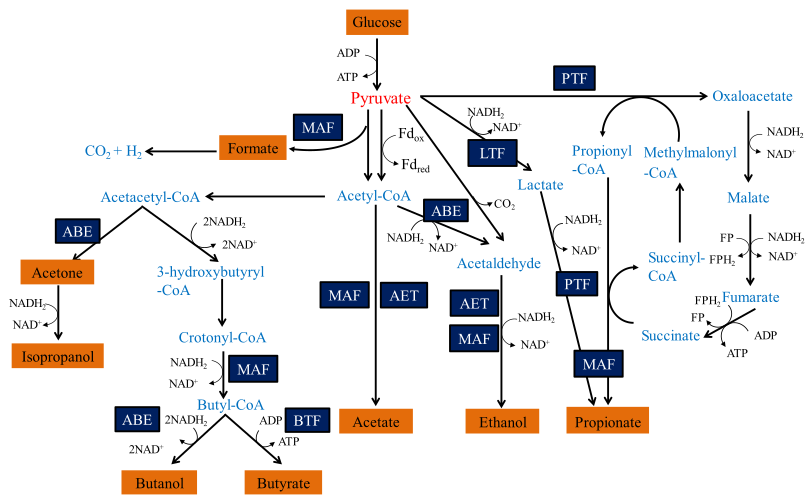
\includegraphics[width=.9\linewidth]{../plots/metabolic_results/pyruvate_metabolism_zhou.png}
\caption[Μεταβολικά μονοπάτια κατανάλωσης του πυροσταφυλικού οξέος]{\label{fig:org0f00bfb}Μεταβολικά μονοπάτια κατανάλωσης του πυροσταφυλικού οξέος (\citeprocitem{102}{Zhou et al. 2018})}
\end{figure}

Στο σύστημα μετά την οξείδωση της γλυκόζης επικρατούν αναγωγικές συνθήκες. Οπότε, είναι πολύ πιθανό να διεξαχθούν αναγωγικές αντιδράσεις. Η απλούστερη αναγωγική αντίδραση είναι η αναγωγή του πυροσταφυλικού οξέος σε γαλακτικό οξύ. Σε πολλές περιπτώσεις, το γαλακτικό οξύ μπορεί να αναχθεί περαιτέρω σε προπιονικό οξύ μέσω του \acrshort{nadh}. Γενικά, το γαλακτικό οξύ επικρατεί σε όξινα pH (4.0-5.0) ενώ με την αύξηση του pH παράγεται περισσότερο προπιονικό. Βέβαια, ακόμη και στα pH που το γαλακτικό επικρατεί, λόγω του υψηλού αναγωγικού φορτίου που είναι διαθέσιμο, θα παραχθεί κάποια ποσότητα προπιονικού. Το μονοπάτι αυτό λέγεται ομογαλακτική ζύμωση, επειδή παράγονται 2 mol γαλακτικού ανά mol γλυκόζης, σε αντίθεση με την ετερογαλακτική ζύμωση όπου παράγεται 1 mol γαλακτικού ανά mol γλυκόζης (\citeprocitem{102}{Zhou et al. 2018}; \citeprocitem{83}{Wu et al. 2015}) .

Το προπιονικό μπορεί να παραχθεί και από άλλο ένα μονοπάτι, το transcarboxylase cycle, το οποίο είναι ένα κυκλικό μονοπάτι μεταξύ οργανικών οξέων με 4 άνθρακες, το οποίο ξεκινάει λόγω της εναλλαγής ενός CO\textsubscript{2} μεταξύ του πυροσταφυλικού οξέος και του μεθυλομηλονικού οξέος, το οποίο μετατρέπεται σε προπιονικό οξύ λόγω αυτού. Ως μεταβολικό προϊόν, μπορεί να παραχθεί σε μεγάλο εύρος pH, αλλά δεν είναι πουθενά το κύριο προϊόν καθώς οι μικροοργανισμοί που παράγουν προπιονικό οξύ αναστέλλονται ισχυρά από το προπιονικό οξύ (\citeprocitem{102}{Zhou et al. 2018}) . Γενικά, είναι σπάνιο να συσσωρευθεί οποιοδήποτε από τα ενδιάμεσα του κύκλου αυτού, αλλά με το κατάλληλο μικροβιακό πληθυσμό, σε ουδέτερο προς αλκαλικό pH (7-8.5) και συσσώρευση CO\textsubscript{2}, μπορεί να παρατηρηθεί συσσώρευση ηλεκτρικού οξέος στον αντιδραστήρα (\citeprocitem{74}{Temudo, Kleerebezem, and van Loosdrecht 2007}) . Ο λόγος που αν συσσωρευτεί κάτι, θα είναι το ηλεκτρικό οξύ, είναι επειδή αυτό αποτελεί το στάδιο του κύκλου το οποίο περιορίζει τον ρυθμό, οπότε αν διακοπεί κάπου ενδιάμεσα, θα είναι στο στάδιο αυτό (\citeprocitem{47}{Mu et al. 2023}) .

Η άλλη βασική αντίδραση κατανάλωσης του πυροσταφυλικού, είναι η οξείδωση του σε \acrshort{acet-coa}. Αυτή δεν καταλύεται από το \acrshort{nad} καθώς στις αναγωγικές συνθήκες που επικρατούν αυτό βρίσκεται στην μορφή του \acrshort{nadh}, αλλά από ένα είδος πρωτεϊνών γνωστές ως \acrfull{fd}. Οι πρωτεΐνες αυτές αποτελούνται από σίδηρο και χαλκό και συνεισφέρουν σε καταλυτικές αντιδράσεις, ανάλογα με την οξειδωτική κατάσταση του σιδήρου. Είναι πιο ισχυρό οξειδοαναγωγικό μέσο από το \acrshort{nad}, οπότε μπορεί να καταλύσει την αντίδραση αυτή παρότι το περιβάλλον είναι αρκετά αναγωγικό (\citeprocitem{80}{Wang, Chen, et al. 2022}; \citeprocitem{102}{Zhou et al. 2018}; \citeprocitem{65}{Sekoai et al. 2018}) . Η αντίδραση αυτή παράγει και ένα mol CO\textsubscript{2} και H\textsubscript{2} κατά την οξείδωση. Οι δύο ενώσεις αυτές βρίσκονται σε ισορροπία με το μυρμηκικό οξύ \(H_2 + CO_2 \rightleftharpoons HCOOH\). Η αντίδραση αυτή έχει \acrfull{dg} αρκετά κοντά στο 0, οπότε, το αν τα δύο αέρια θα είναι σε ελεύθερη μορφή ή θα μετατραπούν σε μυρμηκικό οξύ εξαρτάται σε μεγάλο βαθμό από τις συνθήκες. Η βασικότερη εξάρτηση είναι το pH. Το μυρμηκικό οξύ παρατηρείται γενικά σε pH από 7 και πάνω, ενώ σε χαμηλότερες τιμές η μετατροπή είναι θερμοδυναμικά ανέφικτη. Ο ρόλος του μυρμηκικού οξέος στο σύστημα είναι ότι είναι ένα εναλλακτικό αναγωγικό μέσο, όταν το υδρογόνο δεν είναι στην ελεύθερη μορφή. Δεν συμμετέχει σε άλλες μεταβολικές αντιδράσεις οξεογένεσης (\citeprocitem{74}{Temudo, Kleerebezem, and van Loosdrecht 2007}) .

Από το \acrshort{acet-coa} παράγονται τα υπόλοιπα προϊόντα της διεργασίας. Το πιο "εύκολο" μεταβολικό προϊόν είναι το οξικό οξύ. Παράγεται απευθείας από το \acrshort{acet-coa} ανεξάρτητα από το \acrfull{redox} και σε μεγάλο εύρος pH. Οπότε, είναι το κύριο προϊόν του \acrshort{acet-coa} εκτός αν λόγω συνθηκών επικρατήσει κάποιο άλλο (\citeprocitem{16}{Dai et al. 2017}; \citeprocitem{56}{Qiao et al. 2020}) . Επίσης, οξικό οξύ παράγεται ως συμπροϊόν των αναγωγικών προϊόντων (γαλακτικό και προπιονικό) για να εξισορροπήσει το \acrshort{orp}.

Τα άλλα βασικά προϊόντα από το \acrshort{acet-coa} είναι η αιθανόλη και το βουτυρικό οξύ. Η αιθανόλη παράγεται από την αναγωγή του \acrshort{acet-coa} με ενδιάμεσο την φορμαλδεΰδη. Μεγάλες ποσότητες αιθανόλης παρατηρούνται σε πολύ όξινα pH (4.0-4.5) και ξανά εμφανίζονται σε αλκαλικά pH (8.0) (\citeprocitem{21}{Feng, Li, and Zheng 2018}; \citeprocitem{85}{Wu et al. 2017}; \citeprocitem{74}{Temudo, Kleerebezem, and van Loosdrecht 2007}) . Η ισορροπία αιθανόλης/οξικού είναι μία αρκετά ενδιαφέρουσα ισορροπία. Η αιθανόλη παράγεται από το \acrshort{acet-coa} οπότε η παραγωγή οξικού οξέος ως συμπροϊόν της δεν γίνεται για εξισορρόπηση του \acrshort{orp}. Όμως, συνήθως δεν υπάρχει αρκετό αναγωγικό δυναμικό για να παραχθεί μόνο αιθανόλη. Το πιο συχνά παρατηρούμενο είναι 1 mol γλυκόζης να μετατραπεί σε ένα ισομοριακό μείγμα αιθανόλης και οξικού οξέος, επειδή όλο το αναγωγικό δυναμικό χρησιμοποιείται για την παραγωγή ενός mol αιθανόλης και άρα το άλλο \acrshort{acet-coa} μετατρέπεται σε οξικό. Το μονοπάτι αυτό ονομάζεται ζύμωση αιθανόλης-οξικού (\citeprocitem{102}{Zhou et al. 2018}; \citeprocitem{16}{Dai et al. 2017}; \citeprocitem{85}{Wu et al. 2017}) . 

Το βουτυρικό οξύ παράγεται από το acetacetyl-CoA, το οποίο είναι το προϊόν της αντίδρασης 2 mol \acrshort{acet-coa}. Μετά από δύο αναγωγές, αυτό μετατρέπεται σε butyryl-CoA, το οποίο μετατρέπεται αυθόρμητα σε βουτυρικό οξύ. Έτσι, το βουτυρικό οξύ είναι το μόνο από τα κύρια προϊόντα του μεταβολισμού του πυροσταφυλικού οξέος το οποίο απαιτεί 2 mol πυροσταφυλικού για να παραχθεί. Αποτελεί το κύριο συμπροϊόν του οξικού οξέος σε pH από 5 εώς 6.5. Παράγεται ως συμπροϊόν του οξικού επειδή όπως και για την αιθανόλη, συχνά δεν φτάνει το αναγωγικό δυναμικό για να παραχθεί μόνο του και κάποια mol \acrshort{acet-coa} θα μετατραπούν σε οξικό (\citeprocitem{102}{Zhou et al. 2018}; \citeprocitem{56}{Qiao et al. 2020}; \citeprocitem{21}{Feng, Li, and Zheng 2018}) .

Στην περίπτωση που το pH ξεπεράσει το 6.5, σταματάει να επικρατεί κάποιο οξεογενετικό προϊόν και προτιμάται το μονοπάτι γνωστό ως ζύμωση μικτών οξέων, όπου παράγονται: μυρμηκικό, οξικό, προπιονικό, βουτυρικό και βαλερικό οξύ σε κάποια περιεκτικότητα. Αυτό είναι το μεταβολικό μονοπάτι που ακολουθείται και στην περίπτωση που η οξεογένεση διεξάγεται ταυτόχρονα με την μεθανογένεση, καθώς αυτό είναι το pH στο οποίο διεξάγεται η μεθανογένεση. Αυτό το μονοπάτι δεν είναι ιδιαίτερα επιθυμητό στην περίπτωση που ελέγχεται η οξεογένεση, επειδή προτιμάται ένα πιο ελεγχόμενο προφίλ προϊόντων (\citeprocitem{74}{Temudo, Kleerebezem, and van Loosdrecht 2007}; \citeprocitem{102}{Zhou et al. 2018}; \citeprocitem{56}{Qiao et al. 2020}) .

Ένα τελευταίο μονοπάτι, το οποίο αξίζει να σημειωθεί, παρόλο που δεν παρατηρείται σε μία τυπική οξεογενή ζύμωση είναι η \acrfull{abe}. Η αιθανόλη έχει ήδη αναφερθεί ως προϊόν της οξεογενετικής ζύμωσης. Όπως φαίνεται στο \figurename \ref{fig:org0f00bfb}, η βουτανόλη παράγεται από την αναγωγή του butyryl-CoA σε ισορροπία με το βουτυρικό οξύ, αντίστοιχη με αυτήν του οξικού με την αιθανόλη. Η ακετόνη, είναι εναλλακτικό προϊόν του Acetacetyl-CoA. Ο μηχανισμός της ζύμωσης αυτής είναι πως ξεκινάει με οξεογένεση και συγκεκριμένα ζύμωση οξικού-βουτυρικού, καθώς διεξάγεται συνήθως σε pH 5.5-6.0, όπου επικρατούν τα δύο αυτά προϊόντα, και σταδιακά μετατρέπεται σε διαλυτογένεση (solventogenesis), όπου το acetyl-CoA παράγει αιθανόλη ενώ το acetacetyl-CoA παράγει ακετόνη και βουτανόλη. Βέβαια, για να γίνει αυτό απαιτούνται κάποια ειδικά βακτήρια τα οποία έχουν το μονοπάτι της διαλυτογένεσης. Αυτά είναι μία κατηγορία των βακτηρίων του γένους Clostridium (\citeprocitem{95}{Zhang, Ling, and Huo 2021}; \citeprocitem{102}{Zhou et al. 2018}) .

\section{Αλλα μονοπάτια μεταβολισμού της γλυκόζης}
\label{sec:org2fdece0}
Το μονοπάτι \acrshort{emp} το οποίο έχει αναλυθεί έως τώρα είναι το πιο συχνό μονοπάτι μεταβολισμού της γλυκόζης. Όμως, δεν είναι το μοναδικό μονοπάτι στο οποίο μπορεί να μεταβολιστεί η γλυκόζη. Στο σχήμα \figurename \ref{fig:org82e98c3} φαίνονται όλα τα μεταβολικά μονοπάτια μεταβολισμού της γλυκόζης (\citeprocitem{21}{Feng, Li, and Zheng 2018}) .

\begin{figure}[htbp]
\centering
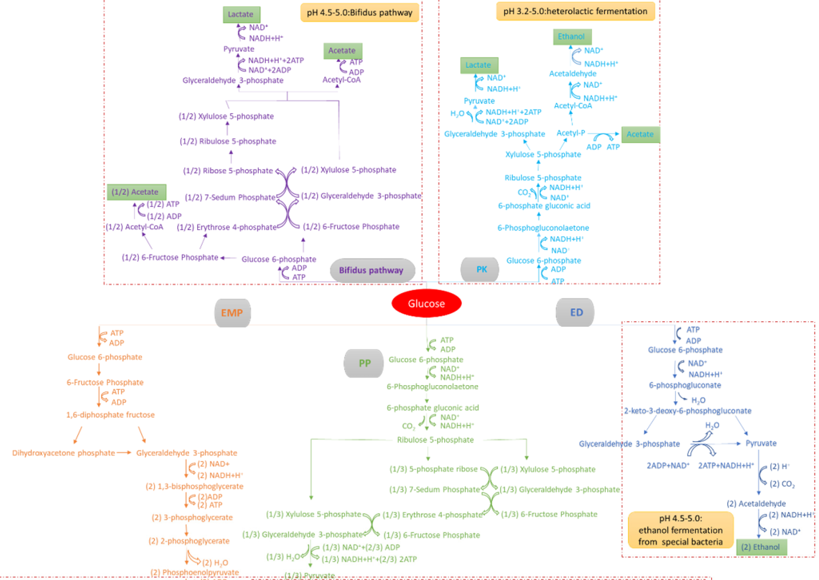
\includegraphics[width=.9\linewidth]{../plots/metabolic_results/glucose_metabolism_qiao.png}
\caption[Μεταβολικά Μονοπάτια της Γλυκόζης]{\label{fig:org82e98c3}Μεταβολικά Μονοπάτια της Γλυκόζης (\citeprocitem{56}{Qiao et al. 2020})}
\end{figure}

Το \acrfull{ed} είναι το μονοπάτι παραγωγής 2 mol αιθανόλης από ένα mol γλυκόζης και υπάρχει κυρίως σε ζύμες. Παρατηρείται σπανίως σε μικτές καλλιέργειες βακτηρίων όπως αυτές που χρησιμοποιούνται στην \acrshort{ad} δύο σταδίων. Το \acrfull{pp} είναι ένα μονοπάτι παρόμοιο του \acrshort{emp} καθώς κάθε mol γλυκόζη μετατρέπεται σε 1/3 mol πυροσταφυλικό και 2/3 mol fructose 6-P το οποίο μπορεί να μεταβολιστεί σε πυροσταφυλικό (\citeprocitem{21}{Feng, Li, and Zheng 2018}; \citeprocitem{56}{Qiao et al. 2020}) .

Τα άλλα 2 μονοπάτια που παρουσιάζονται στο \figurename  \ref{fig:org82e98c3} είναι και τα σημαντικότερα. Το \acrfull{pk}, γνωστό και ως ετερογαλακτική ζύμωση είναι ένα μονοπάτι στο οποίο παράγονται ως τελικά προϊόντα ένα μείγμα γαλακτικού οξέος και αιθανόλης, ή σπανίως οξικού οξέος. Στο μονοπάτι αυτό, παράγεται η ένωση Xylulose 5-Phosphate μετά από 2 οξειδώσεις με αποτέλεσμα να υπάρχει περίσσεια αναγωγικού φορτίου. Η ένωση αυτή διασπάται σε Glyceraldehyde 3-Phosphate - ένωση από την οποία μπορεί να παραχθεί πυροσταφυλικό - και \acrshort{acet-coa}. Καθώς υπάρχει πολύ αναγωγικό δυναμικό στο μονοπάτι αυτό, είναι αρκετά σπάνιο να παραχθεί οξικό οξύ, οπότε παράγεται γαλακτικό οξύ από το πυροσταφυλικό και αιθανόλη από το \acrshort{acet-coa}. Αυτό το μονοπάτι έχει την ιδιαιτερότητα ότι λειτουργεί συνήθως σε pH 4.0-5.0, αλλά μπορεί να γίνει και σε pH κάτω από 4.0 ιδιαίτερα αποτελεσματικά (\citeprocitem{21}{Feng, Li, and Zheng 2018}; \citeprocitem{56}{Qiao et al. 2020}) . Από άποψη μικροβιακής ποικιλότητας, αυτό το μονοπάτι γίνεται από διάφορα βακτήρια, κυρίως του γένους Lactobacillus, τα οποία είναι ιδιαίτερα ενεργά σε \acrshort{fw}. Για αυτό είναι ιδιαίτερα συχνό μονοπάτι όταν χρησιμοποιείται αυτό το υπόστρωμα (\citeprocitem{22}{Feng et al. 2020}; \citeprocitem{83}{Wu et al. 2015}) .

Το μονοπάτι Bifidus είναι παρόμοιο του \acrshort{pk}, καθώς και σε αυτό παράγεται 1 mol Xylulose-5-phosphate. Η βασική διαφορά είναι το πως φτάνει στην ένωση αυτή. Δεν υπάρχει κανένα οξειδωτικό βήμα, με αποτέλεσμα το αναγωγικό δυναμικό στην περίπτωση αυτή να είναι πολύ χαμηλό. Οπότε, το Acetyl-CoA θα μετατραπεί σε οξικό, ενώ το πυροσταφυλικό θα μετατραπεί σε γαλακτικό λόγω του σταδίου οξείδωσης του glyceraldehyde 3-phosphate σε πυροσταφυλικό, το οποίο δημιουργεί αναγωγικό δυναμικό που πρέπει να αξιοποιηθεί. Μία ακόμη διαφορά του μονοπατιού αυτού είναι πως ο ένας άνθρακας που αποβάλλεται για να δημιουργηθεί το Xylulose-5-phosphate δεν γίνεται CO\textsubscript{2}, αλλά μισό mol \acrshort{acet-coa}, το οποίο μετατρέπεται και αυτό σε οξικό, με αποτέλεσμα κάθε mol γλυκόζης να δίνει 1.5 mol οξικό και 1 mol γαλακτικό. Το μονοπάτι αυτό γίνεται σε λίγο πιο υψηλά pH από το \acrshort{pk} όπως 4.5-5.5 (\citeprocitem{56}{Qiao et al. 2020}; \citeprocitem{83}{Wu et al. 2015}) . 

\section{Απόκριση της οξεογένεσης}
\label{sec:org48f575d}
Έχοντας εξετάσει όλα τα δυνατά μονοπάτια της οξεογενετικής ζύμωσης, φτάνει τώρα να εισαχθούν κάποια ποσοτικά στοιχεία για το πως κρίνεται η ποιότητα της οξεογένεσης. Ένα βασικό κριτήριο είναι προφανώς το προφίλ των προϊόντων (\citeprocitem{14}{Chen et al. 2015}; \citeprocitem{22}{Feng et al. 2020}). Άλλωστε, αν δεν είχε σημασία το προφίλ αυτό, δεν θα υπήρχε ενδιαφέρον στον έλεγχο του μονοπατιού της οξεογένεσης. Η ποιότητα όμως του κάθε προϊόντος για την αναερόβια χώνευση θα αναλυθεί στο \autoref{sec:methanogenesis}.

Ένα άλλο, πιο γενικό κριτήριο για να κριθεί η οξεογένεση είναι τα \acrfull{tvfa}. Συγκεκριμένα, αν αυτά εκφραστούν στο ισοδύναμο \acrshort{cod} τους, μπορούν να συγκριθούν με το \acrshort{scod}. Σε μία καλή οξεογένεση, ο λόγος \acrfull{tvfa} προς \acrshort{scod}, ο οποίος είναι γνωστός ως οξίνιση του αντιδραστήρα είναι \(80-90 \%\) (\citeprocitem{14}{Chen et al. 2015}; \citeprocitem{20}{Fang et al. 2020}) .

\chapter{Οξικογένεση και Μεθανογένεση}
\label{sec:orga95eea8}
\label{sec:methanogenesis}

Στα προηγούμενα κεφάλαια αναλύθηκαν εις βάθος η υδρόλυση και η οξεογένεση, τα 2 πρώτα στάδια της \acrshort{ad}, τα οποία είναι και αυτά που συνήθως διαχωρίζονται όταν η διεργασία διεξάγεται σε 2 στάδια. Συγκεκριμένα, στο \autoref{sec:acidogenesis} αναλύθηκαν όλα τα πιθανά μονοπάτια οξεογένεσης και τα προϊόντα του καθενός, και αναφέρθηκε πως είναι επιθυμητό να ελεγχθεί το μεταβολικό μονοπάτι που θα ακολουθηθεί, επειδή δεν είναι όλα τα προϊόντα το ίδιο χρήσιμα για την μεθανογένεση. Για να επεξηγηθεί αυτό, θα πρέπει να εξεταστεί σε βάθος ο μηχανισμός με τον οποίο διεξάγεται η μεθανογένεση, το οποίο είναι ο σκοπός του κεφαλαίου αυτού.
\section{Μηχανισμός Μεθανογένεσης}
\label{sec:orga2afb4f}
Η μεθανογένεση είναι το σημαντικότερο αλλά και πιο ευαίσθητο στάδιο της αναερόβιας χώνευσης. Γίνεται από μικροοργανισμούς του κλάδου των αρχαίων, οι οποίοι είναι υποχρεωτικά αναερόβιοι μικροοργανισμοί με στενό λειτουργικό εύρος pH (περίπου 6.4-8.0). Τα αρχαία τα οποία παράγουν μεθάνιο διαχωρίζονται σε δύο βασικές κατηγορίες, τους ακετοκλαστικούς μεθανογόνους (\acrshort{am}), οι οποίοι χρησιμοποιούν το οξικό οξύ ως υπόστρωμα και τους υδρογονοτρόφους μεθανογόνους (\acrshort{hm}), οι οποίοι ανάγουν διοξείδιο του άνθρακα σε μεθάνιο παρουσία υδρογόνου. Σε κανονικές συνθήκες, περίπου 2/3 του μεθανίου παράγονται από τους \acrshort{am} ενώ τα υπόλοιπα από τους \acrshort{hm} (\citeprocitem{37}{Li et al. 2015}; \citeprocitem{47}{Mu et al. 2023}) .

Για να έχουν υπόστρωμα οι μικροοργανισμοί αυτοί, πρέπει όλα τα προϊόντα της οξεογένεσης να μετατραπούν σε οξικό οξύ και υδρογόνο. Για αυτό υπάρχει το στάδιο της οξικογένεσης. Στο στάδιο αυτό, τα διάφορα προϊόντα που παράχθηκαν κατά την οξεογένεση μετατρέπονται σε οξικό οξύ, ενώ ταυτόχρονα παράγεται και υδρογόνο, καθώς όλες οι αντιδράσεις αυτές είναι οξειδωτικές. Σε αντίθεση όμως με τα 2 προηγούμενα και το επόμενο στάδιο, τα οποία γίνονται αυθόρμητα αν υπάρχει το κατάλληλο μικροβιακό δυναμικό, υπόστρωμα και λειτουργικές συνθήκες, οι περισσότερες οξικογενετικές αντιδράσεις δεν είναι αυθόρμητες σε καμία περιοχή του λειτουργικού εύρους που εξετάζεται (\citeprocitem{53}{Pipyn and Verstraete 1981}) . Ο μηχανισμός με τον οποίο διεξάγονται οι αντιδράσεις αυτές είναι γνωστός ως συντροφικός μεταβολισμός. Για κάθε ένα από τα συχνά προϊόντα της οξεογένεσης, το άθροισμα των αντιδράσεων οξικογένεσης και παραγωγής μεθανίου από οξικό οξύ και υδρογόνο έχει αρνητική \acrshort{dg}, δηλαδή είναι αυθόρμητο. Οπότε, μπορεί να γίνει η αντίδραση οξικογένεσης, η οποία δεν είναι επιθυμητή για το σύστημα, επειδή τα προϊόντα της θα μεταβολιστούν από τους μεθανογόνους και ο συνδυασμός θα είναι ενεργειακά ωφέλιμος (\citeprocitem{70}{Supaphol et al. 2011}; \citeprocitem{37}{Li et al. 2015}; \citeprocitem{53}{Pipyn and Verstraete 1981}) .

Με βάση αυτό, ένα από τα βασικά κριτήρια για την ποιότητα ενός προϊόντος για αναερόβια χώνευση, είναι η θερμοδυναμική των αντιδράσεων αυτών, η οποία θα αναλυθεί παρακάτω.

\section{Θερμοδυναμική Παραγωγής Μεθανίου}
\label{sec:org99d7aa4}
Τα προϊόντα τα οποία θα συζητηθούν εδώ θα είναι τα εξής: Οξικό οξύ, προπιονικό οξύ, γαλακτικό οξύ, βουτυρικό οξύ, αιθανόλη. Τα υπόλοιπα προϊόντα που μπορούν να παραχθούν από οξεογένεση ή δεν παράγονται σε μεγάλη ποσότητα (πχ βαλερικό οξύ), ή όταν παράγονται, ο σκοπός της διεργασίας δεν είναι η παραγωγή μεθανίου (πχ ακετόνη ή βουτανόλη) (\citeprocitem{53}{Pipyn and Verstraete 1981}; \citeprocitem{95}{Zhang, Ling, and Huo 2021}; \citeprocitem{36}{Kohn and Boston 2000}) . Ως αρχικό υπόστρωμα θα εξεταστεί η γλυκόζη, καθώς τα σάκχαρα είναι και το συχνότερο υπόστρωμα της \acrshort{ad}, ενώ αντίστοιχα λειτουργεί και ο μεταβολισμός άλλων υποστρωμάτων.

Η μετατροπή της γλυκόζης σε μεθάνιο (\(C_6H_{12}O_6 \rightarrow 3CH_4 + 3CO_2\)) είναι μία αυθόρμητη αντίδραση με \acrshort{dg} = - 404 kJ/mol σε πρότυπες συνθήκες (\citeprocitem{53}{Pipyn and Verstraete 1981}) . Από τον νόμο του Hess, είναι γνωστό πως η ενθαλπία (και κατ'επέκτασιν η ελεύθερη ενέργεια Gibbs) μίας αντίδρασης είναι ίδια ανεξαρτήτως του μονοπατιού με το οποίο έγινε η αντίδραση. Οπότε, ανεξαρτήτως του ενδιαμέσου, το σύστημα της \acrshort{ad} θα παράγει αυτή την ενέργεια για αυτήν την μετατροπή. Όμως, όσο πιο κοντά στο 0 είναι το άθροισμα των \acrshort{dg} της οξικογένεσης και μεθανογένεσης, τόσο πιο δύσκολο είναι να ολοκληρωθεί η αντίδραση με βάση το μονοπάτι αυτό, με αποτέλεσμα η \acrshort{ad} να μην λειτουργεί σωστά. Ακόμη, οι \acrshort{dg} που θα αναφερθούν παρακάτω είναι σε πρότυπες συνθήκες. Σε διαφορετικά pH (δηλαδή συγκέντρωση υδρογονοκατιόντων) ή σε διαφορετική συγκέντρωση του κάθε προϊόντος, μπορεί η \acrshort{dg} της αντίδρασης να είναι διαφορετική. Οπότε, αν είναι κοντά στο 0 σε πρότυπες συνθήκες, είναι πιθανόν να υπάρχει συνθήκη όπου η αντίδραση δεν μπορεί πλέον να συνεχίσει.

\begin{enumerate}
\item Οξικό Οξύ:
\label{sec:orga262796}
Το οξικό οξύ είναι το ιδανικό υπόστρωμα για μεθανογένεση καθώς είναι το μόνο που μεταβολίζεται απευθείας σε μεθάνιο. Οι αντιδράσεις μεθανογένεσης που διεξάγονται είναι οι

\begin{subequations}
\label{eqn:methanogenesis}
\begin{align}
2CH_3COO^- + 2H_2O &\rightarrow 2CH_4 + 2HCO_3^- & \text{ΔG = - 62.0 kJ} \label{eqn:acet-methane} \\
4H_2 + HCO_3^- + H^+ &\rightarrow CH_4 + 3H_2O & \text{ΔG = -135.6 kJ} \label{eqn:hydro-methane} \\
\hline
2CH_3COO^- + 4H_2 + H^+ &\rightarrow 3 CH_4 + HCO_3^- + H_2O & \text{ΔG = -197.6 kJ} \label{eqn:complete-methane}
\end{align}
\end{subequations}

με αποτέλεσμα το στάδιο αυτό να είναι αυθόρμητο με \acrshort{dg} = -197.6 kJ, δηλαδή σχεδόν η μισή ενέργεια που παράγεται κατά την μετατροπή της γλυκόζης σε μεθάνιο να οφείλεται στην μεθανογένεση (αξίζει να αναφερθεί πως οι συντελεστές είναι με βάση τις ποσότητες που παράγει 1 mol γλυκόζη) (\citeprocitem{53}{Pipyn and Verstraete 1981}) .

\item Προπιονικό Οξύ:
\label{sec:org40a80c5}
Το προπιονικό οξύ είναι συχνό αναγωγικό προϊόν του μεταβολισμού του πυροσταφυλικού οξέος και παρατηρείται συχνά στην \acrshort{ad} (\citeprocitem{16}{Dai et al. 2017}; \citeprocitem{102}{Zhou et al. 2018}) . Εκτός από τις αντιδράσεις \ref{eqn:acet-methane}, \ref{eqn:hydro-methane}, γίνεται και η αντίδραση

\begin{align}
2CH_3CH_2COO^- + 6H_2O &\rightarrow 2CH_3COO^- + 2HCO_3^- + 2H^+ + 6H_2 & \text{ΔG = + 152.2 kJ}
\label{eqn:prop-acet}
\end{align}

με αποτέλεσμα, το άθροισμα οξεογένεσης και μεθανογένεσης να είναι -45.4 kJ και μόνο ένα \(11.4 \%\) της συνολικής ενέργειας να οφείλεται στην μεθανογένεση. Η αντίδραση αυτή παραμένει αυθόρμητη, όμως αποτελεί μία πολύ πιο δύσκολη αντίδραση, διότι οι μεθανογόνοι σπαταλούν πολύ περισσότερη ενέργεια για να διεξαχθεί (\citeprocitem{53}{Pipyn and Verstraete 1981}; \citeprocitem{47}{Mu et al. 2023}). Επιπλέον, σε συνθήκες μακριά από τις πρότυπες (πχ μεγάλη μερική πίεση υδρογόνου ή πολύ όξινο περιβάλλον), η \acrshort{dg} την αντίδρασης \ref{eqn:prop-acet} θα είναι ακόμη μεγαλύτερη, με αποτέλεσμα το άθροισμα να είναι ακόμη πιο κοντά στο 0. Σε ακραίες περιπτώσεις, έχει παρατηρηθεί και κατάρρευση του συστήματος της \acrshort{ad} επειδή έχει παραχθεί πολύ προπιονικό οξύ και στις συνθήκες που υπάρχουν, δεν μπορεί να μετατραπεί σε μεθάνιο. Οπότε, το προπιονικό οξύ είναι γενικά ένα αρκετά ανεπιθύμητο προϊόν (\citeprocitem{52}{Patón, Hernández, and Rodríguez 2020}; \citeprocitem{53}{Pipyn and Verstraete 1981}; \citeprocitem{81}{Wang et al. 2009}) . Όμως, καθώς αποτελεί το βασικότερο αναγωγικό προϊόν της οξεογένεσης, συχνά δεν μπορεί να αποφευχθεί πλήρως (\citeprocitem{102}{Zhou et al. 2018}). Στην βιβλιογραφία, έχουν προταθεί τρόποι για να γίνει πιο εύκολη η αντίδραση αυτή και να μην αναστέλλει το σύστημα, όπως η προσθήκη σιδήρου μηδενικού σθένους (\acrshort{zvi}), ο οποίος μειώνει αρκετά το \acrshort{redox} του αντιδραστήρα, το οποίο κάνει πολύ πιο αρνητικό το \acrshort{dg} της αντίδρασης (\citeprocitem{11}{Cheng et al. 2020}) αλλά και άλλες τεχνολογίες όπως η προσθήκη κάποιου buffer, ή απαραίτητων ιχνοστοιχείων για να γίνει πιο αποτελεσματική η αντίδραση (\citeprocitem{47}{Mu et al. 2023}) .

\item Γαλακτικό Οξύ:
\label{sec:orgda7c325}
Το άλλο συχνό αναγωγικό προϊόν είναι το γαλακτικό οξύ, το οποίο όπως αναφέρθηκε, παράγεται σε μεγάλες ποσότητες κατά την ζύμωση \acrshort{fw} (\citeprocitem{22}{Feng et al. 2020}; \citeprocitem{83}{Wu et al. 2015}) . Το γαλακτικό οξύ είναι ένα ενδιαφέρον ενδιάμεσο για την \acrshort{ad} καθώς η αναγωγή του σε προπιονικό οξύ και η οξείδωση του σε οξικό είναι και οι δύο κοντά στην ισορροπία. Σε πρότυπες συνθήκες είναι οι εξής: (\citeprocitem{53}{Pipyn and Verstraete 1981}; \citeprocitem{63}{Saady 2013})

\begin{subequations}
\label{eqn:lact-redox}
\begin{align}
2CH_3CHOHCOO^- &\rightarrow 2CH_3COO^- + 2HCO_3^- + 2H^+ + 4H_2 & \text{ΔG = - 8.4 kJ} \label{eqn:lact-ox} \\
2CH_3CHOHCOO^- &\xrightarrow{2NADH \rightarrow 2NAD^+} 2CH_3CH_2COO^- & \text{ΔG = 27.6 kJ} \label{eqn:lact-red}
\end{align}
\end{subequations}

Επίσης υπενθυμίζεται πως το ζεύγος \acrshort{nadh} με \acrshort{nad} είναι ένα οξειδωαναγωγικό ζεύγος με την ισορροπία

\begin{align}
NADH + H^+ &\rightleftharpoons NAD^+ + H_2 & ΔG = - 21.8 \frac{kJ}{mol}
\label{eqn:nadh}
\end{align}

Άρα, σε πρότυπες συνθήκες, θερμοδυναμικά επιθυμητή είναι η αντίδραση \ref{eqn:lact-ox}, οπότε θεωρητικά θα έπρεπε το γαλακτικό οξύ να είναι ένα ιδιαίτερα επιθυμητό προϊόν της \acrshort{ad}. Όμως, η \acrshort{ad} λειτουργεί σε ένα αρκετά αναγωγικό περιβάλλον, όπου το \acrshort{nadh} είναι συχνότερα στην ανηγμένη μορφή του και άρα η \ref{eqn:lact-red} ευνοείται πολύ περισσότερο, ενώ η \ref{eqn:lact-ox} έχει γίνει θερμοδυναμικά ανέφικτη. Βέβαια, η συντροφική δράση των μικροοργανισμών αυτών με τους μεθανογόνους κάνει την αντίδραση αυτή εφικτή, όπως και για τα άλλα προϊόντα. Στην πράξη, o πιο συχνός μεταβολισμός του γαλακτικού οξέος είναι ένας μικτός μεταβολισμός με βάση την αντίδραση

\begin{align}
3CH_3CHOHCOOH &\rightarrow 2CH_3CH_2COOH + CH_3COOH + HCO_3^- + H^+ & \text{ΔG = -165 kJ}
\label{eqn:mixed-lact}
\end{align}

Η αντίδραση αυτή είναι μία οξειδωαναγωγική αντίδραση όπου τα υδρογόνα της \ref{eqn:lact-ox} χρησιμοποιούνται για την \ref{eqn:lact-red} με αποτέλεσμα μία ιδιαίτερα θερμοδυναμική επιθυμητή αντίδραση. Αυτή είναι η αντίδραση που ακολουθείται όταν και οι δύο αντιδράσεις είναι πολύ κοντά σε ισορροπία (\citeprocitem{63}{Saady 2013}) . 

Οπότε, το γαλακτικό οξύ δεν είναι ένα ιδιαίτερα επιθυμητό ενδιάμεσο, λόγω της πιθανότητας να μεταβολιστεί σε προπιονικό (\citeprocitem{53}{Pipyn and Verstraete 1981}), αλλά υπό τις κατάλληλες συνθήκες αποτελεί ένα πολύ καλό ενδιάμεσο της διεργασίας και κάποιες μελέτες έχουν δείξει πολύ καλή απόδοση στην \acrshort{ad} από υπόστρωμα πλούσιο σε γαλακτικό (\citeprocitem{11}{Cheng et al. 2020}; \citeprocitem{22}{Feng et al. 2020}) .

\item Βουτυρικό Οξύ:
\label{sec:orgbaaf305}
Το βουτυρικό οξύ είναι ένα ακόμη σύνηθες προϊόν της οξεογένεσης (\citeprocitem{14}{Chen et al. 2015}; \citeprocitem{102}{Zhou et al. 2018}) . Η οξικογένεση του βουτυρικού είναι η αντίδραση

\begin{align}
CH_3CH_2CH_2COO^- + 2H_2O &\rightarrow 2CH_3COO^- + H^+ + 2H_2 & \text{ΔG = + 48.1 kJ}
\label{eqn:but-ox}
\end{align}

Η αντίδραση αυτή δεν είναι αυθόρμητη σε πρότυπες συνθήκες, αλλά σε συντροφικό μεταβολισμό με τις αντιδράσεις \ref{eqn:methanogenesis} έχει ένα τελικό \acrshort{dg} = -149.5 kJ (\citeprocitem{63}{Saady 2013}; \citeprocitem{53}{Pipyn and Verstraete 1981}). Γενικά το βουτυρικό οξύ είναι ένα προϊόν το οποίο μετατρέπεται εύκολα σε μεθάνιο λόγω αυτού και υπάρχουν μελέτες που έχουν δείξει πως είναι ένα από τα πιο επιθυμητά προϊόντα της οξεογένεσης (\citeprocitem{102}{Zhou et al. 2018}; \citeprocitem{81}{Wang et al. 2009}; \citeprocitem{14}{Chen et al. 2015}) .

\item Αιθανόλη:
\label{sec:org5ee2633}
Η αιθανόλη είναι το τελευταίο προϊόν το οποίο θα εξεταστεί. Αποτελεί ένα αναγωγικό προϊόν του \acrshort{acet-coa} που παράγεται ως συμπροϊόν του οξικού οξέος σε χαμηλά pH (\citeprocitem{56}{Qiao et al. 2020}; \citeprocitem{102}{Zhou et al. 2018}) . Η αιθανόλη μπορεί να μετατραπεί σε οξικό αρκετά εύκολα για τον λόγο αυτό. Η αντίστοιχη αντίδραση είναι η

\begin{align}
2C_2H_5OH + 2H_2O &\rightarrow 2CH_3COO^- + 2H^+ + 4H_2 & \text{ΔG = + 19.2 kJ}
\label{eqn:eth-acet}
\end{align}

η οποία έχει θετική αλλά χαμηλή \acrshort{dg} με αποτέλεσμα σε συνδυασμό με τις αντιδράσεις \ref{eqn:methanogenesis} να έχει \acrshort{dg} = -178.4 kJ, το οποίο καθιστά την μετατροπή της αιθανόλης σε μεθάνιο αρκετά εύκολη. Ακόμη, σε ορισμένες συνθήκες (χαμηλή μερική πίεση υδρογόνου, υψηλή συγκέντρωση αιθανόλης) μπορεί η αντίδραση αυτή να γίνει αυθόρμητη και από μόνη της και να παρατηρηθεί οξικογένεση χωρίς συντροφική μεθανογένεση (\citeprocitem{53}{Pipyn and Verstraete 1981}; \citeprocitem{63}{Saady 2013}) . 

Εκτός από το γεγονός ότι είναι ένα ενδιάμεσο που μετατρέπεται εύκολα σε μεθάνιο και άρα είναι καλό για μεθανογένεση (\citeprocitem{22}{Feng et al. 2020}; \citeprocitem{104}{Zhu, Zhao, and Zhang 2019}), η αιθανόλη έχει δείξει να βελτιώνει την ρυθμιστική ικανότητα του αντιδραστήρα (\citeprocitem{92}{Yu et al. 2018}) και να προάγει το μεταβολικό μονοπάτι \acrfull{diet} για την μεθανογένεση, το οποίο είναι πολύ ενεργειακά αποτελεσματικό (\citeprocitem{103}{Zhu et al. 2022}; \citeprocitem{98}{Zhao and Zhang 2019}; \citeprocitem{60}{Rotaru et al. 2013}) . Τα πλεονεκτήματα του μονοπατιού αυτού έναντι του συμβατικού (\acrfull{iht}) θα αναλυθούν περισσότερο παρακάτω.
\end{enumerate}

\section{Πλεονεκτήματα του Direct Interspecies Electron Transfer στην Mεθανογένεση}
\label{sec:orgbfa83f8}
Το συμβατικό μοντέλο συντροφικού μεταβολισμού μεταξύ των οξικογόνων μικροοργανισμών και των μεθανογόνων, βασίζεται στην παραγωγή οξικού οξέος αλλά και υδρογόνου, η μεθανογένεση των οποίων προσφέρει στο σύστημα την απαιτούμενη ενέργεια για να λειτουργήσει (\citeprocitem{63}{Saady 2013}; \citeprocitem{53}{Pipyn and Verstraete 1981}) . Ο ρόλος του υδρογόνου είναι η αναγωγή του CO\textsubscript{2} σε CH\textsubscript{4}. Ένα αναγωγικό μέσο είναι μία ένωση που προσφέρει ηλεκτρόνια σε άλλες ενώσεις. Οπότε, ουσιαστικά το υδρογόνο δρα ως ένας φορέας ηλεκτρονίων τον οποίο δημιουργούν οι οξικογόνοι για να επιτρέψουν αναγωγικές αντιδράσεις στους μεθανογόνους. Ο μηχανισμός αυτός λέγεται \acrfull{iht} (\citeprocitem{63}{Saady 2013}; \citeprocitem{60}{Rotaru et al. 2013}) .

Όμως, το υδρογόνο δεν αποτελεί το κύριο προϊόν της οξείδωσης. Το κύριο προϊόν μίας οξειδωτικής αντίδρασης είναι τα ηλεκτρόνια, τα οποία παράγουν το υδρογόνο για να μεταφέρουν την αναγωγική τους ιδιότητα σε κάποια ένωση. Στην πράξη, όλες οι οξικογενετικές αντιδράσεις είναι οξειδωαναγωγικές αντιδράσεις, των οποίων η αναγωγική ημί-αντίδραση είναι η

\begin{align}
2H^+ + 2e^- &\rightleftharpoons H_2 & \text{ΔG = 856.9 kJ/mol}
\label{eqn:hydrogen}
\end{align}

Για παράδειγμα, η οξικογένεση από προπιονικό οξύ είναι στην ουσία το άθροισμα των αντιδράσεων

\begin{subequations}
\label{eqn:prop-redox}
\begin{align}
2CH_3CH_2COO^- + 6H_2O \rightarrow 2CH_3COO^- + 2HCO_3^- + 14H^+ + 12e^-  \label{eqn:prop-ox} \\
12H^+ + 12e^- \rightarrow 6H_2 \label{eqn:hydro-red} \\
\hline
2CH_3CH_2COO^- + 6H_2O \rightarrow 2CH_3COO^- + 2HCO_3^- + 2H^+ + 6H_2 \label{eqn:prop-acet-comp}
\end{align}
\end{subequations}

Το πρόβλημα, έγκειται στο γεγονός ότι η θερμοδυναμική ευνοεί τον ιοντισμό του υδρογόνου σε υδρογονοκατιόντα και ηλεκτρόνια, αλλά δεν ευνοεί την αντιστροφή της αντίδρασης αυτής. Σε μία παρόμοια λογική με παραπάνω, η αντίδραση αυτή γίνεται επειδή το σύστημα θα κερδίσει ενέργεια αν παραχθεί υδρογόνο, μεταφερθεί στους \acrshort{hm} και αυτοί το μεταβολίσουν. Όμως, αν μπορούσαν να μεταφερθούν απευθείας τα ηλεκτρόνια και να ανάγουν αυτά το CO\textsubscript{2} κατά την μεθανογένεση, το σύστημα θα ήταν πολύ πιο αποδοτικό ενεργειακά (\citeprocitem{60}{Rotaru et al. 2013}) .

Αυτό είναι το μεταβολικό μονοπάτι \acrfull{diet}, στο οποίο παρακάμπτεται η παραγωγή υδρογόνου και τα ηλεκτρόνια μεταφέρονται απευθείας. Το μονοπάτι αυτό παρατηρήθηκε πρώτη φορά μεταξύ του ζεύγους μικροοργανισμών των γενών Geobacter (οξικογόνοι) και Methanosaeta (ακετοκλαστικοί μεθανογόνοι) από τους (\citeprocitem{60}{Rotaru et al. 2013}) κατά την επεξεργασία υγρών αποβλήτων ζυθοποιίας. Με μία μικροβιακή ανάλυση, παρατηρήθηκε πως οι \acrshort{hm} ήταν λιγότερο από \(1 \%\) των αρχαίων, όμως, ενώσεις όπως η αιθανόλη μεταβολιζόντουσαν κανονικά. Ακόμη, η παραγωγή μεθανίου ήταν περισσότερη από ότι θα μπορούσε να είναι αν μόνο το οξικό μετατρεπόταν σε μεθάνιο. Μετά από διερεύνηση, βρέθηκαν γονίδια αναγωγής του CO\textsubscript{2}, παρότι η αναγωγή δεν γινόταν από υδρογόνο. Οπότε, υποτέθηκε πως τα ηλεκτρόνια μεταφέρονται απευθείας από την μία ομάδα μικροοργανισμών στην άλλη.

Μετά την δημοσίευση αυτή, έγινε πολύ περισσότερη έρευνα πάνω στον μηχανισμό αυτόν. Βρέθηκε πως και άλλοι μικροοργανισμοί μπορούν να συμμετέχουν σε αυτόν τον μεταβολισμό (\citeprocitem{59}{Rotaru et al. 2014}) και διαπιστώθηκε πειραματικά πως ο λόγος που βρέθηκε πρώτα σε απόβλητα ζυθοποιίας είναι επειδή η αιθανόλη ενεργοποιεί το μονοπάτι αυτό, όχι μόνο αν υπάρχει εξαρχής εκεί, αλλά και στην περίπτωση που γίνει ένα ethanol-type fermentation κατά την οξεογένεση (\citeprocitem{101}{Zhao, Zhang, Yu, et al. 2016}; \citeprocitem{99}{Zhao et al. 2017}; \citeprocitem{98}{Zhao and Zhang 2019}) . Αυτό είναι ιδιαίτερα ενδιαφέρον για όξινα απόβλητα όπως τα \acrshort{fw} επειδή σε μία αναερόβια χώνευση σε 2 στάδια, είναι συχνό ένα από τα κύρια προϊόντα της οξεογένεσης να είναι η αιθανόλη και άρα να ενεργοποιηθεί το \acrshort{diet} (\citeprocitem{91}{Ye et al. 2018}; \citeprocitem{103}{Zhu et al. 2022}) . Ακόμη, βρέθηκε πως εκτός από την αιθανόλη, η προσθήκη αγώγιμων ενώσεων ή πρόσθετων μπορεί να ενεργοποιήσει και να ενισχύσει το μονοπάτι αυτό για ακόμη καλύτερη αποδοτικότητα. Υλικά όπως ο ενεργός άνθρακας, το biochar ή ο \acrshort{zvi} μελετήθηκαν στην διεργασία αυτή και φάνηκε πως την βελτιώνουν (\citeprocitem{91}{Ye et al. 2018}; \citeprocitem{103}{Zhu et al. 2022}; \citeprocitem{31}{Jiang, Zhao, and Zhang 2022}) .

Εκτός όμως από τα πλεονεκτήματα του \acrshort{diet} ενεργειακά, έχει παρατηρηθεί πως μπορεί να βοηθήσει και στην ρυθμιστική ικανότητα του αντιδραστήρα (\citeprocitem{92}{Yu et al. 2018}; \citeprocitem{103}{Zhu et al. 2022}) αλλά και στην αντοχή του σε μεγάλες συγκεντρώσεις \acrshort{vfa}, υψηλά \acrshort{olr} και υψηλή μερική πίεση υδρογόνου. Ως αποτέλεσμα, η μεθανογένεση μέσω του \acrshort{diet} είναι πολύ πιο σταθερή, εκτός από αποτελεσματική (\citeprocitem{31}{Jiang, Zhao, and Zhang 2022}; \citeprocitem{101}{Zhao, Zhang, Yu, et al. 2016}; \citeprocitem{100}{Zhao, Zhang, Holmes, et al. 2016}) .

\section{Απόκριση της μεθανογένεσης}
\label{sec:orgc017e11}
\label{sec:gompertz}

Παραπάνω αναφέρθηκε η ποιότητα του κάθε προϊόντος για την μεθανογένεση σε θεωρητικό επίπεδο. Στην πράξη, για να μετρηθεί η ποιότητα ενός υποστρώματος για μεθανογένεση, χρησιμοποιείται το \acrfull{bmp} ή κάποια άλλη παρόμοια δοκιμή. Σκοπός αυτών είναι μία batch δοκιμή στην οποία μπορεί να υπάρξει εύκολη 24ωρή παρατήρηση της αναερόβιας χώνευσης και μπορούν να εξεταστούν πολλά υποστρώματα ταυτόχρονα. Έτσι, μπορεί να γίνει μία ανάλυση της μέγιστης ποσότητας μεθανίου που μπορεί να παράξει κάθε υπόστρωμα (είτε ανά gCOD που καταναλώνεται ή ανά gVS λάσπης του αντιδραστήρα) καθώς και του ρυθμού παραγωγής τους. Έτσι, μπορεί να προκύψει το βέλτιστο υπόστρωμα από όσα θα εξεταστούν (\citeprocitem{14}{Chen et al. 2015}; \citeprocitem{22}{Feng et al. 2020}; \citeprocitem{19}{Dhar, Nakhla, and Ray 2012}; \citeprocitem{27}{Hobbs et al. 2018}) .

Στην περίπτωση του ρυθμού παραγωγής, ο προσδιορισμός αυτού απαιτεί την επιλογή ενός κινητικού μοντέλου. Για αυτό έχουν προταθεί πολλά μοντέλα, όπως το λογιστικό μοντέλο, το μοντέλο κώνου, το μοντέλο Richards και το μοντέλο Gompertz (\citeprocitem{22}{Feng et al. 2020}; \citeprocitem{107}{Zwietering et al. 1990}; \citeprocitem{92}{Yu et al. 2018}; \citeprocitem{69}{Sunyoto et al. 2016}) . Οι (\citeprocitem{107}{Zwietering et al. 1990}) έδειξαν πως το μοντέλο Gompertz, το οποίο περιγράφεται από την εξίσωση \ref{eqn:gompertz}

\begin{equation}
y = a\exp [-\exp(b-cx)]
\label{eqn:gompertz}
\end{equation}

είναι ένα μοντέλο το οποίο έχει αρκετή πολυπλοκότητα για να περιγράψει πολύ αναλυτικά την βακτηριδιακή ανάπτυξη (σε αντίθεση με απλούστερα μοντέλα όπως το λογιστικό), ενώ μοντέλα με μεγαλύτερη πολυπλοκότητα (πχ περισσότερες παραμέτρους όπως το μοντέλο Richards) δεν βελτιώνουν ιδιαίτερα την απόδοση της προσαρμογής. Συγκεκριμένα, προτείνουν μία τροποποίηση του μοντέλου ώστε οι 3 σταθερές του να αποκτήσουν φυσικό νόημα. Η εξίσωση που προκύπτει είναι η

\begin{equation}
y = A \exp \left[ -\exp \left( \frac{μ_{\max }e}{Α} (λ-t) + 1 \right) \right]
\label{eqn:mod-gompertz}
\end{equation}

στην οποία η σταθερά Α είναι το πλατό της καμπύλης της μικροβιακής ανάπτυξης (στάσιμη φάση), η σταθερά μ\textsubscript{max} είναι ο μέγιστος ειδικός ρυθμός ανάπτυξης της μικροβιακής διεργασίας και λ ο χρόνος καθυστέρησης της.

Το μοντέλο αυτό έχει χρησιμοποιηθεί ευρέως για την μοντελοποίηση της μεθανογένεσης με πολύ καλά αποτελέσματα (\citeprocitem{34}{Khadka et al. 2022}; \citeprocitem{27}{Hobbs et al. 2018}; \citeprocitem{20}{Fang et al. 2020}; \citeprocitem{22}{Feng et al. 2020}; \citeprocitem{75}{Uçkun Kiran, Trzcinski, and Liu 2015}) .

\part{Πειραματικό Μέρος}
\label{sec:org5a6a56e}

\chapter{Υλικά και Μέθοδοι}
\label{sec:org55375de}
\label{sec:materials_methods}

\section{Υπόστρωμα και Εμβόλιο}
\label{sec:org33b0882}
Τα \acrshort{fw} που χρησιμοποιήθηκαν συλλέχθηκαν από την φοιτητική λέσχη του Εθνικού Μετσόβιου Πολυτεχνείου και αποθηκεύτηκαν στους - 20 \(^oC\) για περαιτέρω χρήση. Για τα εργαστηριακά πειράματα, όπου χρειάστηκε μικρή ποσότητα υποστρώματος ανά πείραμα, συλλέχθηκαν τρόφιμα μία φορά και τεμαχίστηκαν σε μπλέντερ (Cecotec Powder Black Titanium 2000). Έτσι, επιτεύχθηκε μία ομοιόμορφη ημιστερεή φάση η οποία μπορεί να χρησιμοποιηθεί ως υπόστρωμα για την υδρόλυση. Το υλικό αυτό αναλύθηκε ως προς το pH, την ηλεκτρική αγωγιμότητα, τα στερεά, την πυκνότητα και το \acrfull{cod}. Η σύσταση του φαίνεται στον πίνακα \ref{tab:orgabd8aa5}. Στην διάταξη της πιλοτικής κλίμακας, ο τεμαχισμός δεν ήταν απαραίτητος καθώς ο αντιδραστήρας είχε την δυνατότητα αυτή. Λόγω των ποσοτήτων που χρειαζόντουσαν, υπήρχε καθημερινή συλλογή \acrshort{fw}, τα χαρακτηριστικά των οποίων δεν αναλύθηκαν.

\begin{table}[htbp]
\caption{\label{tab:orgabd8aa5}Χαρακτηριστικά Υπολειμμάτων Τροφών}
\centering
\begin{tabular}{ll}
Παράμετροι & Τιμή\\[0pt]
\hline
pH & 4.62 \textpm{} 0.02\\[0pt]
EC (μS/cm) & 1817.7 \textpm{} 38.0\\[0pt]
TS (\%) & 11.54 \textpm{} 2.18\\[0pt]
VS (\%) & 10.93 \textpm{} 2.07\\[0pt]
VS/TS (\%) & 94.70 \textpm{} 4.46\\[0pt]
Density (g/mL) & 1.0316 \textpm{} 0.0078\\[0pt]
sCOD (mg/L) & 20009 \textpm{} 1980\\[0pt]
TCOD (mg/L) & 96031 \textpm{} 2204\\[0pt]
sCOD/tCOD(\%) & 20.82 \textpm{} 1.58\\[0pt]
\end{tabular}
\end{table}

Το \acrfull{mix} που χρησιμοποιήθηκε είναι το εμπορικό σκεύασμα PROGEN L 100 της εταιρείας NCR Biochemical. Το σκεύασμα αυτό έχει ειδικά επιλεγμένους μικροοργανισμούς του γένους Bacillus οι οποίοι είναι ιδιαίτερα ενεργοί και είναι ικανοί να μεταβολίσουν οργανικά απόβλητα. Ιδιαίτερη έμφαση δίνεται στον μεταβολισμό λιπαρών ενώσεων, οι οποίες είναι και αυτές που δημιουργούν πρόβλημα σε βιολογικές δράσεις αν δεν αποδομηθούν. Καθώς το σκεύασμα είναι εμπλουτισμένο με ένζυμα, υδρολύει και έπειτα μεταβολίζει το απόβλητα ταχύτατα. Αυτό το κάνει ιδανικό για την πιο αποτελεσματική εκκίνηση ή την υποβοήθηση μίας βιολογικής δράσης, όπως για παράδειγμα η αναερόβια χώνευση. Είναι φιλικό προς το περιβάλλον καθώς οι μικροοργανισμοί που περιέχει επηρεάζουν θετικά το οικοσύστημα στο οποίο θα απορριφθούν.

Για την \acrshort{ad} χρησιμοποιήθηκε αναερόβια λάσπη προερχόμενη από τρεις διαφορετικές πηγές. Η πρώτη (Λάσπη 1) από τo \acrfull{kel} των βορείων προαστίων της Αττικής, η δεύτερη (Λάσπη 2) από μονάδα ανακύκλωσης απορριμάτων στην Βοιωτία και η τρίτη (Λάσπη 3) από αναερόβιο χωνευτήρα εγκατεστημένο σε βιομηχανία τροφίμων στην Αττική. Οι λάσπες αυτές αναλύθηκαν ως προς τα στερεά, το pH και την αλκαλικότητα. Τα αποτελέσματα των αναλύσεων αυτών φαίνονται στον πίνακα \ref{tab:org8b524fd}. 

\begin{table}[htbp]
\caption{\label{tab:org8b524fd}Χαρακτηριστικά Λάσπης}
\centering
\begin{tabular}{llll}
Παράμετροι & Λάσπη 1 & Λάσπη 2 & Λάσπη 3\\[0pt]
\hline
TS (g/kg) & 46.277 \textpm{} 0.033 & 25.546 \textpm{} 0.238 & 4.315 \textpm{} 0.151\\[0pt]
VS (g/kg) & 12.364 \textpm{} 0.322 & 16.148 \textpm{} 0.704 & 2.001 \textpm{} 0.072\\[0pt]
VS/TS (\%) & 26.72 \textpm{} 0.72 & 63.23 \textpm{} 3.34 & 46.38 \textpm{} 0.05\\[0pt]
pH & 8.33 \textpm{} 0.01 & 8.90 \textpm{} 0.07 & 7.50 \textpm{} 0.03\\[0pt]
Αλκαλικότητα (mg/L) & 12250 & 14200 & 1100\\[0pt]
\end{tabular}
\end{table}

Η Λάσπη 3 είναι κοκκώδης λάσπη από αντιδραστήρα \acrshort{uasb}. Οπότε, παρότι έχει χαμηλή αλκαλικότητα και στερεά, θεωρείται πως έχει καλή ενεργότητα και μπορεί να χρησιμοποιηθεί αποτελεσματικά για μία αναερόβια χώνευση.

\section{Πειραματική διάταξη υδρόλυσης εργαστηριακής κλίμακας}
\label{sec:org739db04}
Τα πειράματα υδρόλυσης/βιοαποδόμησης σε εργαστηριακή κλίμακα έγιναν στο όργανο DT70 της PHARMA TEST. Η διάταξη αυτού φαίνεται στο \figurename \ref{fig:orga43bb22}. 

\begin{figure}[htbp]
\centering
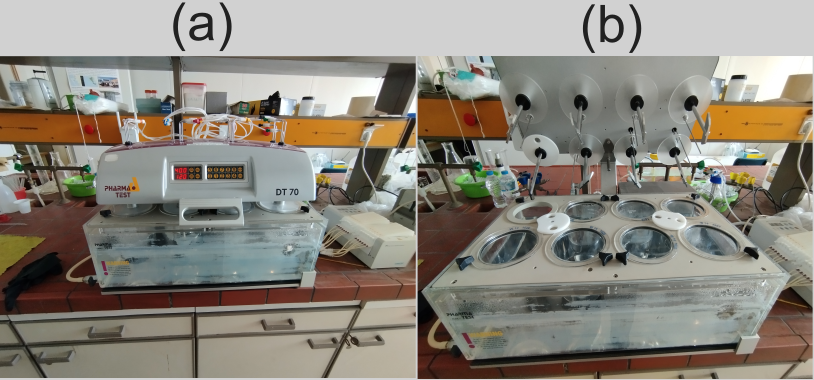
\includegraphics[width=.9\linewidth]{./lab_scale_hydrolysis.png}
\caption{\label{fig:orga43bb22}Πειραματική Διάταξη Υδρόλυσης Εργαστηριακής Κλίμακας}
\end{figure}

Συγκεκριμένα, το σύστημα αυτό αποτελείται από 7 ανεξάρτητα δοχεία χωρητικότητας 1 L, τα οποία είναι τοποθετημένα σε υδατόλουτρο για ρύθμιση της θερμοκρασίας και είναι εξοπλισμένα με αναδευτήρες τύπου κουπιού (Σχήμα \ref{fig:orga43bb22} (b)). Η θερμοκρασία και η ανάδευση ρυθμίζονται από μία οθόνη την οποία διαθέτει το μηχάνημα (Σχήμα \ref{fig:orga43bb22} (a)). 

Ένα από τα βασικά πλεονεκτήματα μίας τέτοιας διάταξης είναι η ευκολία να δοκιμαστούν ταυτόχρονα πολλές λειτουργικές συνθήκες, καθώς το κάθε δοχείο λειτουργεί ανεξάρτητα. Έτσι, είναι η ιδανική διάταξη για την βελτιστοποίηση μίας τέτοιας διεργασίας.

\section{Δοκιμαστικά πειράματα υδρόλυσης}
\label{sec:org30f3106}
\label{sec:prep-hydro}

Για να αποφανθούν οι σημαντικότερες συνθήκες λειτουργίας της διεργασίας υδρόλυσης/βιοαποδόμησης έγιναν κάποια δοκιμαστικά πειράματα.

Το πρώτο δοκιμαστικό πείραμα χρησιμοποίησε τα \acrfull{ss} και το \acrfull{scod} ως βασικές αποκρίσεις. Η λογική αυτού ήταν πως τα \acrshort{ss} θα πρέπει να μειώνονται καθώς γίνεται υδρόλυση, ενώ δεν θα επηρεάζονται από αυξήσεις που οφείλονται στην ανάπτυξη των μικροοργανισμών και το \acrshort{scod} θα αυξάνεται καθώς γίνεται υδρόλυση και η στερεή οργανική ύλη διαλύεται. Εξετάστηκαν διαφορετικές αναλογίες \acrshort{fw}-νερού (1:1, 1:2 και 1:3), κρατώντας την ποσότητα \acrshort{fw} σταθερή στα 200 g, για να βρεθεί αν το μείγμα παραμένει ομοιογενές και μπορεί να παρατηρηθεί ικανοποιητική υδρόλυση. Η ανάδευση ρυθμίστηκε στα 120 rpm, όπου παρατηρήθηκε πως όλα τα μίγματα αναδευόντουσαν αποτελεσματικά. Η θερμοκρασία ρυθμίστηκε στους 45 \(^oC\), καθώς οι διεργασίες ενζυμικής υδρόλυσης είναι συνήθως αποδοτικές σε θερμοκρασίες κοντά στους 50 \(^oC\). 

Διαπιστώθηκε πως τα \acrfull{ss} μειώνονται σε 24 ώρες, αλλά και το \acrshort{scod} μειώθηκε. Έτσι, προέκυψε το συμπέρασμα πως η υδρόλυση και η ζύμωση διεξάγονται ταυτόχρονα και η ζύμωση έχει γρηγορότερο ρυθμό (εφόσον υπάρχει μείωση στερεών αλλά και μείωση \acrshort{scod}). Επίσης, παρατηρήθηκαν προβλήματα στην διεξαγωγή της διήθησης στις αραιώσεις 1:1 και 1:2, οπότε για όλα τα επόμενα πειράματα χρησιμοποιήθηκε η αραίωση 1:3.

Για να μελετηθεί πιο αναλυτικά η αλληλεπίδραση των δύο διεργασιών και να επιλεχθούν οι κατάλληλες συνθήκες για έναν πειραματικό σχεδιασμό βελτιστοποίησης, έγινε ένα δεύτερο πείραμα. Στο πείραμα αυτό χρησιμοποιήθηκαν 2 επαναλήψεις του ίδιου πειράματος (για να μελετηθεί η επαναληψιμότητα της διεργασίας), στο οποίο χρησιμοποιήθηκε αναλογία \acrshort{fw}-νερού 1:3 και ανάδευση 120 rpm, όπως επιλέχθηκαν από το προηγούμενο πείραμα. Η θερμοκρασία ρυθμίστηκε στους 45 \(^oC\) και προστέθηκαν 2 mL \acrshort{mix}. Ως μεταβλητές απόκρισης, δοκιμάστηκαν οι εξής: \acrshort{ss} (ολικά και πτητικά), \acrshort{scod}, συγκέντρωση σακχάρων και συγκέντρωση προϊόντων οξεογενούς ζύμωσης (συγκεκριμένα μετρήθηκαν γαλακτικό οξύ, οξικό οξύ, προπιονικό οξύ και αιθανόλη). Για να αποφασισθεί η διάρκεια της διεργασίας υδρόλυσης/βιοαποδόμησης, η δειγματοληψία στο πείραμα αυτό ήταν συχνή. Συγκεκριμένα, την πρώτη μέρα έγινε δειγματοληψία στις 0, 1, 2, 3, 4, 5, 6 ενώ τις επόμενες 4 ημέρες, γινόταν δειγματοληψία κάθε 2 ώρες για 6 ώρες. Στο 2ο δείγμα (που χρησιμοποιείται για επανάληψη) δεν έγιναν οι συχνές δειγματοληψίες την πρώτη μέρα, αλλά μόνο δειγματοληψίες στις 0, 1 και 5 ώρες. Καθώς παρατηρήθηκαν αλλαγές μέχρι και την 5η μέρα (98 ώρες), το πείραμα αυτό αφέθηκε να λειτουργήσει και πάρθηκαν 2 τελευταία δείγματα στις 167 και 171 ώρες για να διαπιστωθεί αν θα παρατηρηθεί κάποιο πλατό.

Τέλος, έγινε ένα τρίτο πείραμα, όπου μετρήθηκε κατά βάση η εξάτμιση του νερού, η οποία παρατηρήθηκε πως έπαιξε σημαντικό ρόλο στα προηγούμενα πειράματα. Συγκεκριμένα, καθώς η διάταξη που χρησιμοποιήθηκε έχει 7 θέσεις, τοποθετήθηκαν 7 πανομοιότυπα πειράματα με τις εξής συνθήκες: 200 g FW, 600 g νερό, 2 mL \acrshort{mix}, θερμοκρασία ρυθμισμένη στους 35 \(^oC\) και ανάδευση στα 120 rpm. Μετά από 1, 2, 3, 7, 9, 11 και 14 ημέρες μετά την έναρξη του πειράματος, ένα από τα 7 δείγματα αφαιρούταν από την διάταξη και μετριόταν η μάζα του καθώς και τα TS του. Αφαιρώντας την μείωση μάζας των στερεών (η οποία οφείλεται καθαρά στην υδρόλυση) από την μείωση της συνολικής υγρής μάζας, μπόρεσε να προσδιοριστεί η μείωση της μάζας του νερού. Εφόσον δεν υπήρχαν δειγματοληψίες, η απώλεια μάζας αυτή οφειλόταν αποκλειστικά στην εξάτμιση. Έτσι, ποσοτικοποιήθηκε και ο ρυθμός εξάτμισης.

\section{Πειραματικός κύκλος υδρόλυσης}
\label{sec:orgeabfe86}
\label{sec:lab-hydro}
Με βάση τα αποτελέσματα των δοκιμαστικών πειραμάτων αυτών σχεδιάστηκε ένας πειραματικός κύκλος για την βελτιστοποίηση της διεργασίας. Αποφασίστηκε να μην ρυθμιστεί η αραίωση και η ανάδευση και να αφεθούν στην τιμή που βρέθηκε πως λειτουργεί καλά η διεργασία (200 mL \acrshort{fw}, 600 mL νερό, 120 rpm ανάδευση), ενώ ως παράμετροι προς βελτιστοποίηση επιλέχθηκαν η θερμοκρασία και η ποσότητα του \acrshort{mix}. Για την θερμοκρασία, εξετάστηκαν οι τιμές 35 και 40 \(^oC\) ως δύο αντιπροσωπευτικές τιμές της μεσόφιλης περιοχής, ενώ όπου υπήρχε η δυνατότητα, εξετάστηκε και η διαφορά τους με την θερμοκρασία 45 \(^oC\) όπου έγινε ένα από τα δοκιμαστικά πειράματα. Για την ποσότητα του \acrshort{mix} εξετάστηκαν οι τιμές 0 (επίδραση μόνο της θερμοκρασίας), 1, 2, 4 και 8 ml ανά 200 mL FW. 

Ως μεταβλητές απόκρισης στα πειράματα αυτά επιλέχθηκαν η μέτρηση των συγκεντρώσεων σακχάρων, των \acrshort{vfa} και του \acrshort{scod}.  Με αυτά, μπορούν να υπολογιστούν τα εξής: η συνολική συγκέντρωση \acrshort{vfa} η οποία δείχνει πόσα προϊόντα παράχθηκαν και ιδιαίτερα ο λόγος \(\frac{\text{tVFAs in COD-eq}}{\text{sCOD}}\) ο οποίος είναι ένας πολύ χρήσιμος λόγος για μία διεργασία οξεογένεσης καθώς αποτελεί την απόδοση της. Επίσης, σημαντική είναι και η αναλογία της τελικής υγρής απορροής στα διάφορα \acrshort{vfa}, η οποία είναι καθοριστική για την ποιότητα της αναερόβια χώνευση.

Εκτός από την τελική δειγματοληψία όμως, έγιναν και δειγματοληψίες κατά την διάρκεια του πειράματος (μία φορά την ημέρα, η οποία κρίθηκε η βέλτιστη συχνότητα μετά τα δοκιμαστικά πειράματα). Η δειγματοληψία αυτή επέτρεψε την καταγραφή κάποιων σταδίων στην διεργασία, το οποίο επέτρεψε την διαπίστωση των μεταβολικών μονοπατιών που ακολουθήθηκαν.

\section{Υδρόλυση σε πιλοτική κλίμακα}
\label{sec:org003daa9}
\label{sec:pilot-exp}

Για τα πειράματα σε πιλοτική κλίμακα χρησιμοποιήθηκε ο πρωτότυπος αερόβιος χωνευτήρας (MyECO) χωρητικότητας 300 L. Η διάταξη αυτού φαίνεται στο Σχήμα \ref{fig:org94b896b}.

\begin{figure}[htbp]
\centering
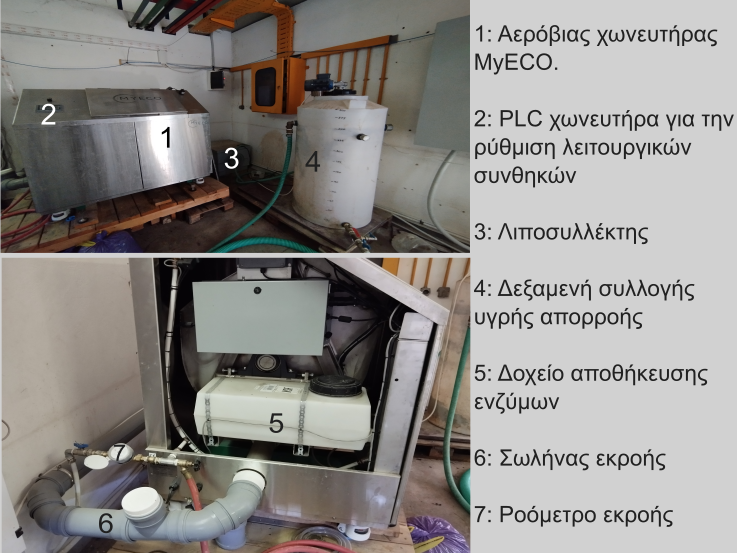
\includegraphics[width=.9\linewidth]{./pilot_hydrolysis_captioned.png}
\caption{\label{fig:org94b896b}Πειραματική Διάταξη Πιλοτικής Υδρόλυσης}
\end{figure}

Στο εσωτερικό του χωνευτήρα έχει τοποθετηθεί αδρανές πλαστικό πληρωτικό υλικό, για την καλύτερη διεπαφή \acrshort{fw} και ενζύμων-μικροοργανισμών καθώς και τον σχηματισμό βιοφίλμ, ο οποίος ανεβάζει την απόδοση επεξεργασίας της χώνευσης. Ακόμη, στο εσωτερικό του χωνευτήρα υπάρχει ένας οριζόντιος άξονας με 4 ράβδους οι οποίες επιτρέπουν τον τεμαχισμό και ταυτόχρονα την ανάδευση του συστήματος. Συγκεκριμένα, οι ράβδοι αυτές έχουν ελαστικά άκρα, όποτε μπορούν να τεμαχίσουν τα υδρολύματα κατά την περιστροφή τους και να τα μεταφέρουν προς την εκροή, αναδεύοντας τα. Το σύστημα αυτό έχει ισχύ 1 HP. Επιπλέον, ο χωνευτήρας διαθέτει εσωτερική ζυγαριά για την μέτρηση της μάζας της τροφοδοσίας και ενσωματωμένο PLC (2) που επιτρέπει την ρύθμιση του ρυθμού τροφοδοσίας του σκευάσματος, το οποίο είναι αποθηκευμένο σε ειδικό δοχείο του οργάνου (5), καθώς και του νερού που προστίθεται στο εσωτερικό του αντιδραστήρα, αλλά και στην εκροή του, για την αραίωση του τελικού προϊόντος. Μετά από κάποιον χρόνο παραμονής, η επεξεργασμένη υγρή εκροή αποβάλλεται από τον χωνευτήρα (6) και οδηγείται σε λιποσυλλέκτη (3) για να απομακρυνθούν οι λιπαρές ενώσεις. Η εκροή αυτού οδηγείται στη δεξαμενή συλλογής χωρητικότητας 300 L (4) από την οποία γίνεται η δειγματοληψία για να αναλυθεί η ποιότητα της εκροής αυτής. Το όργανο διαθέτει ροόμετρο για την μέτρηση της εκροής του (7).

Η λειτουργία του είναι ήμι-διαλείποντος έργου καθώς ο αντιδραστήρας τροφοδοτείται 2 φορές την ημέρα (μία το πρωί και μία το απόγευμα) ενώ η εκροή του λειτουργεί συνεχώς.

Τα πειράματα που διεξάχθηκαν στην κλίμακα αυτή είχαν ως σκοπό να εξετάσουν την εφικτότητα της υδρόλυσης σε μεγαλύτερη κλίμακα και την συλλογή υδρολύματος για αναερόβια χώνευση, για να διαπιστωθεί αν αυτή είναι το ίδιο αποτελεσματική στην εργαστηριακή και πιλοτική κλίμακα. Για τον σκοπό αυτόν, η τροφοδοσία του \acrshort{mix} ρυθμίστηκε σε τιμές οι οποίες αντιστοιχούν στις αναλογίες που χρησιμοποιήθηκαν στα πειράματα εργαστηριακής κλίμακας. Βέβαια, ο πιλοτικός χωνευτήρας δεν έχει την δυνατότητα ελέγχου της θερμοκρασίας, οπότε αναμένεται να μην είναι ακριβώς ίδια η ζύμωση σε σχέση με αυτήν στην εργαστηριακή κλίμακα. Για να εξεταστεί κάποια άλλη λειτουργική συνθήκη του συστήματος, έγινε ένας πειραματικός κύκλος όπου αυξήθηκε η προσθήκη νερού στον χωνευτήρα, για να διαπιστωθεί αν θα επηρεάσει πραγματικά το σύστημα, ή αν θα μειώσει απλώς το \acrshort{cod} λόγω αραίωσης.

Οπότε, οι 3 κύκλοι οι οποίοι διεξάχθηκαν είχαν τις εξής συνθήκες:
\begin{itemize}
\item 1ος κύκλος: Τροφοδοσία 35.8 kg \acrshort{fw}/day με προσθήκη 4.24 L νερό/kg \acrshort{fw} και 0.005 L \acrshort{mix}/kg \acrshort{fw} (αντίστοιχο με το 1 mL στην εργαστηριακή κλίμακα).
\item 2ος κύκλος: Τροφοδοσία 37.5 kg \acrshort{fw}/day με προσθήκη 5.71 L νερό/kg \acrshort{fw} και 0.005 L \acrshort{mix}/kg \acrshort{fw}.
\item 3ος κύκλος: Τροφοδοσία 24.9 kg \acrshort{fw}/day με προσθήκη 8.9 L νερό/kg \acrshort{fw} και 0.01 L \acrshort{mix}/kg \acrshort{fw} (αντίστοιχο με το 2 mL στην εργαστηριακή κλίμακα).

Αξίζει να αναφερθεί πως το νερό είναι σε κάθε περίπτωση περισσότερο από αυτό που χρησιμοποιούταν στα πειράματα εργαστηριακής κλίμακας (3 L νερό/kg \acrshort{fw}). Αυτό συμβαίνει διότι στην πιλοτική διάταξη απαιτείται περισσότερο νερό για να είναι ομοιογενής η λειτουργία και να μην υπάρχουν προβλήματα από ότι στην εργαστηριακή κλίμακα.

Ως απόκριση της διεργασίας, εξετάστηκαν οι παραμέτροι \acrshort{ts}, \acrshort{vs}, \acrshort{scod}, \acrshort{tcod} . Ιδιαίτερα σημαντικό για την διεργασία θεωρήθηκε να είναι υψηλή η αναλογία sCOD/tCOD, η οποία αποτελεί την απόδοση της διεργασίας υδρόλυσης/βιοαποδόμησης.
\end{itemize}

\section{Πειραματική διάταξη αναερόβιας χώνευσης}
\label{sec:org1521e2f}
Η \acrshort{ad} πραγματοποιήθηκε σε εργαστηριακούς αντιδραστήρες διαλείποντος έργου, συνολικού όγκου 500 mL ο καθένας. Η διάταξη που χρησιμοποιήθηκε φαίνεται στο Σχήμα \ref{fig:org98a9629}.

\begin{figure}[htbp]
\centering
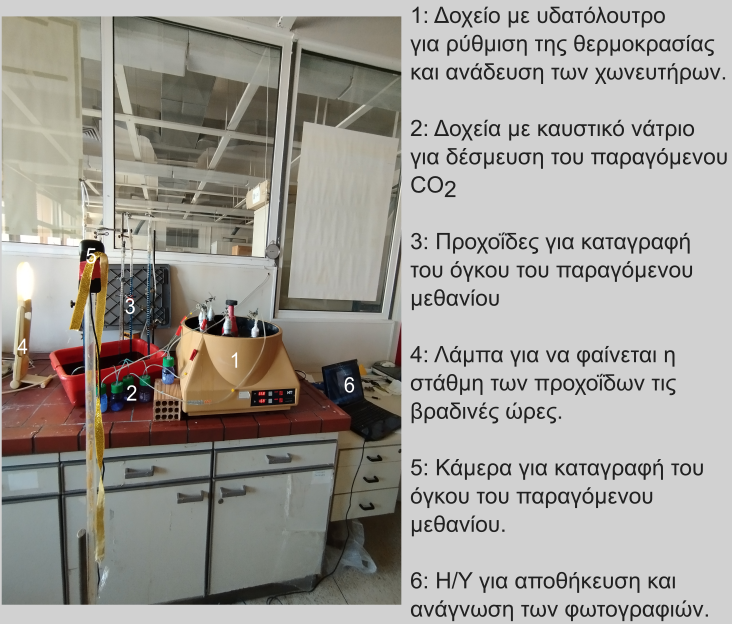
\includegraphics[width=350px]{./anaerobic_digestion_captioned.png}
\caption{\label{fig:org98a9629}Πειραματική Διάταξη Αναερόβιας Χώνευσης}
\end{figure}

Για να διεξαχθεί ένας κύκλος πειραμάτων αναερόβιας χώνευσης, αρχικά ανοίγει το υδατόλουτρο (1) για να φτάσει την επιθυμητή θερμοκρασία και πληρώνονται οι αντιδραστήρες με λάσπη και νερό. Σφραγίζονται με χρήση parafilm και σιλικόνης για να είναι σίγουρο ότι δεν θα μπορέσει να υπάρξει κάποια διαρροή, δηλαδή απώλεια μεθανίου. Για να εκκινήσει η αντίδραση, το υπόστρωμα τροφοδοτείται στον αντιδραστήρα από ειδικό σωληνάκι με χρήση σύριγγας. Μόλις παραχθεί αέριο, αυτό θα διοχετευθεί στα δοχεία με το καυστικό νάτριο (2). Το καυστικό νάτριο μπορεί να δεσμεύσει το διοξείδιο του άνθρακα καθώς αντιδρά με το ανθρακικό οξύ που παράγεται όταν το CO\textsubscript{2} βρεθεί σε υδατική φάση. Ως αποτέλεσμα, στις προχοΐδες (3) διοχετεύεται καθαρό μεθάνιο, το οποίο είναι και αυτό που μας ενδιαφέρει. Η κάμερα (5) καταγράφει μία φορά την ώρα την στάθμη του νερού όλο το 24 ώρο, για να μπορέσει να γίνει μία κινητική μελέτη της διεργασίας αναερόβιας χώνευσης. Για τις βραδινές ώρες, είναι απαραίτητο να είναι ανοιχτή η λάμπα (4), ώστε να μπορεί να διαβαστεί η στάθμη των προχοΐδων. Οι φωτογραφίες που βγαίνουν κάθε ώρα, αποθηκεύονται στον Η/Υ (6), για να μπορέσουν να αναγνωστούν.

Έτσι, με την διάταξη αυτή μπορεί να εξεταστεί εύκολα το \acrfull{bmp} 5 διαφορετικών υποστρωμάτων ταυτόχρονα καθώς και ο ρυθμός παραγωγής μεθανίου σε αυτά ή η \acrfull{sma} τους. 

\section{Πειραματικός κύκλος αναερόβιας χώνευσης}
\label{sec:org5060e2c}
Μετά από βελτιστοποίηση της υδρόλυσης στην εργαστηριακή κλίμακα, αποφασίστηκε πως η θερμοκρασία 40 \(^oC\) είναι πιο αποτελεσματική και ότι οι ποσότητες 1, 2 και 4 έχουν τα καλύτερα αποτελέσματα και αξίζει να διερευνηθούν περαιτέρω. Οπότε, οι 2 πρώτοι πειραματικοί κύκλοι αναερόβιας χώνευσης έγιναν με τα υδρολύματα αυτά για να εξεταστεί η ικανότητα τους να παράξουν μεθάνιο. Έπειτα, έγινε και ένας τρίτος κύκλος στον οποίο εξετάστηκε η ικανότητα παραγωγής μεθανίου από τα υδρολύματα που προήλθαν από την πιλοτική υδρόλυση. Σε όλα τα πειράματα η θερμοκρασία ήταν ρυθμισμένη στους 37 \(^oC\) και η ανάδευση στα 170 rpm.

Κατά τον πρώτο κύκλο πειραμάτων, ο οποίος διεξάχθηκε με την Λάσπη 1, χρησιμοποιήθηκε εμβόλιο 125 g λάσπης (1.55 g VS/αντιδραστήρα) και πλήρωση του αντιδραστήρα με νερό. Αρχικά, η αναερόβια λάσπη ενεργοποιήθηκε με τροφοδοσία οξικού οξέος (100 mg), και στη συνέχεια, ακολούθησε η τροφοδοσία με τα υδρολύματα. Εκτός από τα υδρολύματα με 1, 2 και 4 mL \acrshort{mix}/200 g FW, χρησιμοποιήθηκαν και το δείγμα με 0 mL \acrshort{mix}, το οποίο δείχνει την επίδραση μόνο της θερμοκρασίας, και το ανεπεξέργαστο \acrshort{fw}, για να διαπιστωθεί αν η αναερόβια χώνευση πραγματικά βελτιώνεται με την προσθήκη του \acrshort{mix}. Η τροφοδοσία με υδρολύματα έγινε με 100 mg \acrshort{scod}, δηλαδή μία αναλογία \acrfull{si} 0.06 g COD/g VS. Η αναλογία αυτή είναι σχετικά μικρή σε σχέση με άλλες μελέτες (\citeprocitem{27}{Hobbs et al. 2018}; \citeprocitem{75}{Uçkun Kiran, Trzcinski, and Liu 2015}; \citeprocitem{22}{Feng et al. 2020}), αλλά επιλέχθηκε επειδή δίνει μία άμεση απόκριση, με αποτέλεσμα να μπορούν να γίνουν εύκολα πολλοί πειραματικοί κύκλοι.

Ο δεύτερος κύκλος πειραμάτων έγινε με παρόμοια λογική. Σκοπός ήταν να εξεταστεί αναερόβια λάσπη από διαφορετική πηγή (Λάσπη 2), για να διαπιστωθεί αν υπάρχει επαναληψιμότητα στα πειράματα. Στον κύκλο αυτό προστέθηκε μεγαλύτερο εμβόλιο λάσπης (250 g ή 4.2 g VS) ενώ η ποσότητα των υδρολυμάτων παρέμεινε ίδια (100 mg \acrshort{scod}). Οπότε, η αναλογία \acrshort{si} ήταν 0.02 g COD/g VS.

Στον τρίτο κύκλο χρησιμοποιήθηκαν τα υδρολύματα της πιλοτικής μονάδας. Συγκεκριμένα, χρησιμοποιήθηκαν τα πειράματα P1 και P3, τα οποία ήταν σε ποσότητα \acrshort{mix} ισοδύναμα των πειραμάτων με 1 και 2 ml \acrshort{mix} από την εργαστηριακή κλίμακα. Σκοπός του κύκλου αυτού ήταν να επιβεβαιωθεί η εφικτότητα της παραγωγής μεθανίου από το υδρόλυμα αυτό και η διαφορές που έχει από τα ίδια πειράματα σε εργαστηριακή κλίμακα. Καθώς όμως εξετάστηκαν μόνο 2 υδρολύματα, υπήρξε δυνατότητα να χρησιμοποιηθεί λάσπη από 2 διαφορετικές πηγές στον ίδιο κύκλο, για να διαπιστωθεί η επαναληψιμότητα αυτού. Συγκεκριμένα, χρησιμοποιήθηκε η Λάσπη 2 για να συγκριθούν τα αποτελέσματα με την εργαστηριακή κλίμακα, αλλά χρησιμοποιήθηκε επίσης και η Λάσπη 3. Και στις 2 περιπτώσεις χρησιμοποιήθηκαν 250 g λάσπης, αλλά αυτό ισοδυναμεί σε 4.2 g VS για την Λάσπη 2 και σε 0.5 g VS για την Λάσπη 3.

Ως βασικές αποκρίσεις εδώ, χρησιμοποιήθηκαν η μέγιστη παραγωγή μεθανίου από κάθε δείγμα, καθώς και ο ρυθμός παραγωγής αυτού με βάση το τροποποιημένο μοντέλο Gompertz (\autoref{sec:gompertz}) εφόσον υπήρχε η δυνατότητα 24ωρής καταγραφής του φαινομένου.

\section{Αναλυτικές Μέθοδοι}
\label{sec:org0ad7bb2}
\label{sec:analyses}

Η μέτρηση pH έγινε με χρήση pH μέτρου (inoLab pH Level 1 pH Meter) σε ακολουθία με τις πρότυπες τεχνικές, ενότητα 4500-H\^{}+ (\citeprocitem{2}{APHA, AWWA, and WEF 2005}). Η μέτρηση ηλεκτρικής αγωγιμότητας έγινε με τον ηλεκτροχημικό αναλυτή CONSORT C933.

Η μέτρηση των στερεών, έγινε σε ακολουθία με τις πρότυπες τεχνικές, ενότητα 2540 (\citeprocitem{2}{APHA, AWWA, and WEF 2005}) . Συγκεκριμένα για τα \acrfull{ts}, έγινε ζύγιση σε προ-ζυγισμένη κάψα μετά από ξήρανση σε φούρνο στους 75 \(^oC\) για 1 μέρα, ενώ για να μετρηθούν τα \acrfull{vs}, έγινε ζύγιση μετά από ξήρανση σε φούρνο στους 550 \(^oC\) για 2 ώρες. Για τα \acrfull{ss}, έγινε αρχικά διήθηση του δείγματος με χρήση προ-ζυγισμένου φίλτρου Whatman GF/A το οποίο κατακρατεί στερεά διαμέτρου 1.6 μm και πάνω. Έπειτα, ακολουθήθηκε η ίδια διαδικασία με παραπάνω για την μέτρηση ολικών και πτητικών αιωρουμένων στερεών.

Η μέτρηση του \acrshort{cod} έγινε σε ακολουθία με τις πρότυπες τεχνικές, ενότητα 5220 (\citeprocitem{2}{APHA, AWWA, and WEF 2005}). Για την μέτρηση αυτή, αρχικά γίνεται αραίωση του δείγματος ανάλογα με το αναμενόμενο \acrshort{cod}, καθώς η μέθοδος είναι αξιόπιστη σε COD από 50 έως 1000 mg/L. Έπειτα, 2 ml του αραιωμένου δείγματος αναμιγνύονται με 2.8 ml πυκνού θειικού οξέος και 1.2 ml διχρωμικού καλίου και τοποθετούνται σε ειδικό φούρνο στους 150 \(^oC\) για 2 ώρες (HACH COD Reactor 45600). Το διχρωμικό κάλιο είναι ισχυρό οξειδωτικό, ενώ το θειικό οξύ και η θερμοκρασία δρουν ως καταλύτες της αντίδρασης. Ανάλογα με το \acrshort{cod}, μεταβάλλεται η οξειδωτική κατάσταση του χρωμίου από +6 σε +3. Ταυτόχρονα, μεταβάλλεται το χρώμα του από πορτοκαλί σε γαλάζιο. Μετρώντας την απορρόφηση στα 600 nm μετά τις 2 ώρες, μπορεί να ποσοτικοποιηθεί η οξείδωση που διεξάχθηκε, και άρα το COD του δείγματος. Για να μετρηθεί το \acrshort{cod} ενός δείγματος, απαιτείται μία πρότυπη καμπύλη η οποία αντιστοιχεί την απορρόφηση σε συγκέντρωση \acrshort{cod}. Για την μέτρηση του \acrshort{tcod} το δείγμα λαμβανόταν ως είχε, ενώ για την μέτρηση του \acrshort{scod}, το δείγμα αρχικά διηθούταν με χρήση φίλτρου Whatman. Για ορισμένα δείγματα με πολλά στερεά, γινόταν και μία φυγοκέντριση (EBA 20, Hettich Zentrifugen σε συνθήκες 6000 rpm, 10 λεπτά) για να ολοκληρωθεί πιο γρήγορα ο διαχωρισμός των στερεών.

Για την αλκαλικότητα ακολουθήθηκε η μέθοδος της ογκομέτρησης. Συγκεκριμένα, 20 mL δείγματος ογκομετρήθηκαν με θειικό οξύ κανονικότητας 0.2 Ν μέχρι το pH να φτάσει 4.5. Ο όγκος που απαιτείται (V\textsubscript{sulf}) είναι ενδεικτικός της αλκαλικότητας. Συγκεκριμένα, ισχύει \(\text{Alkalinity} = \frac{50 \cdot 1000 \cdot 0.2 \cdot V_{sulf}}{20}\) με την αλκαλικότητα να μετριέται σε mg CaCO\textsubscript{3}/L.  

Για την μέτρηση των σακχάρων και των πτητικών λιπαρών οξέων κατά την υδρόλυση, χρησιμοποιήθηκε μία στήλη για \acrfull{hplc} (Agilent Technologies Infinity II). Ακολουθήθηκε η μέθοδος lactic temp, η οποία έχει χρόνο παραμονής στην στήλη 45 λεπτά και κινητή φάση HPLC Grade νερό με πυκνό θεϊικό οξύ συγκέντρωσης 275 μL/L. Οι κορυφές που ταυτοποιήθηκαν είναι για τις εξής ενώσεις: γλυκόζη, φρουκτόζη, σακχαρόζη, γαλακτικό οξύ, οξικό οξύ, προπιονικό οξύ και αιθανόλη. Στα χρωματογραφήματα υπήρχαν και κάποιες άλλες κορυφές, αλλά ήταν πολύ μικρές και θεωρήθηκαν αμελητέες. Οι κορυφές που ταυτοποιήθηκαν δεν παρουσίασαν κάποια επικάλυψη και ήταν όλες αρκετά ψηλές για να είναι έμπιστη η μέτρηση τους.

\chapter{Επεξεργασία Αποτελεσμάτων}
\label{sec:orgb402fda}
\label{sec:result_analysis}

Όλα τα πειραματικά αποτελέσματα αναλύθηκαν με την βοήθεια της γλώσσας προγραμματισμού Julia (\citeprocitem{5}{Bezanson et al. 2017}). Η Julia είναι μία ελεύθερα διαθέσιμη γλώσσα η οποία είναι ιδιαίτερα κατάλληλη για υπολογιστικά προβλήματα όπως αυτά που χρειάστηκε να αναλυθούν. Η είσοδος και έξοδος δεδομένων μπορεί να γίνει εύκολα μέσω αρχείων CSV με την χρήση βιβλιοθηκών όπως οι CSV.jl και DataFrames.jl (\citeprocitem{6}{Bouchet-Valat and Kamiński 2023}), κάτι το οποίο επιτρέπει την διαλειτουργικότητα με εργαλεία όπως το Excel το οποίο μπορεί να δημιουργήσει αλλά και να διαβάσει τα αρχεία αυτά. Ακόμη, έχει πολύ καλές δυνατότητες παρουσίασης αποτελεσμάτων λόγω των εξαιρετικών βιβλιοθηκών της για γραφήματα. Στην εργασία αυτή χρησιμοποιήθηκαν τα (\citeprocitem{17}{Danisch and Krumbiegel 2021}; \citeprocitem{15}{Christ et al. 2023}) . Η ανάλυση των αποτελεσμάτων έγινε με επαναλήψιμο τρόπο με την βοήθεια της βιβλιοθήκης DrWatson (\citeprocitem{18}{Datseris et al. 2020}) και ανέβηκε στο \href{https://github.com/Vidianos-Giannitsis/masters-thesis}{GitHub}. Έτσι, κάνοντας clone το repository αυτό, μπορεί οποιοσδήποτε να επαναπαράγει τα αποτελέσματα που θα παρουσιαστούν.

Σκοπός του κεφαλαίου αυτού είναι μία παρουσίαση του τρόπου επεξεργασίας των πειραματικών αποτελεσμάτων της εργασίας ενώ στο επόμενο κεφάλαιο θα γίνει η παράθεση κάποιων συγκεντρωτικών δεδομένων από τα οποία θα μπορέσουν να προκύψουν και τα τελικά συμπεράσματα.

\section{Δοκιμαστικά πειράματα υδρόλυσης}
\label{sec:org0d878bb}
Τα πρώτα πειράματα που έγιναν ήταν τα δοκιμαστικά πειράματα για την υδρόλυση \autoref{sec:prep-hydro}. Αυτά επέτρεψαν την διαπίστωση των βέλτιστων συνθηκών λειτουργίας για τον κύριο πειραματικό κύκλο της υδρόλυσης.

\begin{enumerate}
\item Δοκιμή Διάφορων Αραιώσεων:
\label{sec:orgc9a40bf}
Από το πρώτο πείραμα δεν προέκυψαν πολλά αποτελέσματα, πέρα από το γεγονός ότι υδρόλυση και ζύμωση διεξάγονται ταυτόχρονα με την ζύμωση να υπερισχύει. Αξίζει να αναφερθεί πως από τα πειράματα που έγιναν, στην αραίωση 1:1 δεν μπόρεσε να διηθηθεί το δείγμα (και απορρίφθηκε γενικά ως αραίωση), στην αραίωση 1:2 ολοκληρώθηκε οριακά η διήθηση και στην αραίωση 1:3 διηθήθηκε κανονικά. Παρακάτω παρατίθενται τα διαγράμματα για τα \acrfull{tss} (\ref{fig:orgdec3c5a}) και το \acrfull{scod} (\ref{fig:org4983879}) για το πείραμα αυτό. Τα \acrfull{vss} μετρήθηκαν αλλά δεν παρουσιάζονται καθώς ακολουθούν ακριβώς την ίδια τάση με τα \acrfull{tss}. Συγκεκριμένα, για το πείραμα με αραίωση 1:2 ο λόγος VSS/TSS ήταν \(96.65 \pm 0.50\) και για την αραίωση 1:3 \(97.98 \pm 0.23\). 

\begin{figure}[htbp]
\centering
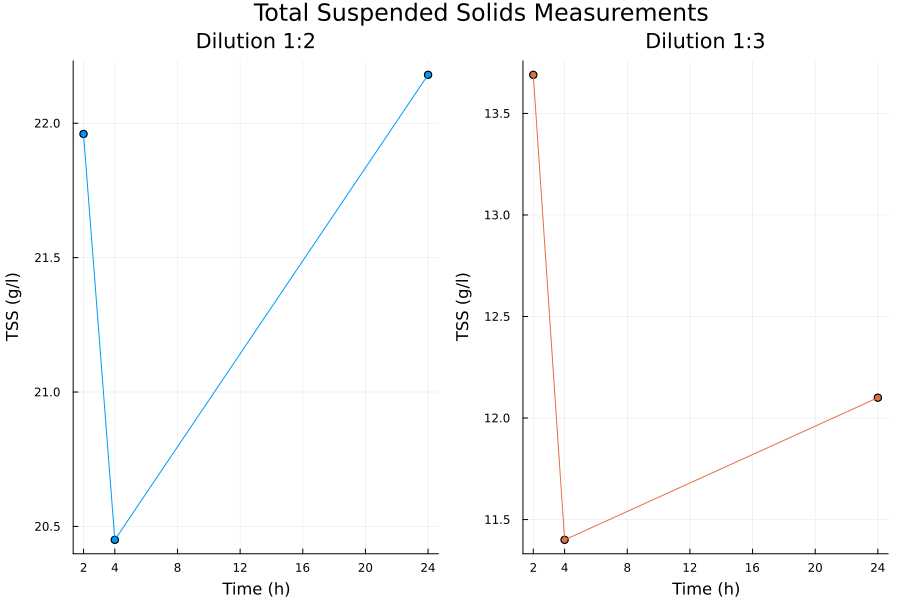
\includegraphics[width=.9\linewidth]{../plots/10_10/tss_plot.png}
\caption{\label{fig:orgdec3c5a}Μέτρηση TSS - Δοκιμαστικό Πείραμα 1}
\end{figure}

\begin{figure}[htbp]
\centering
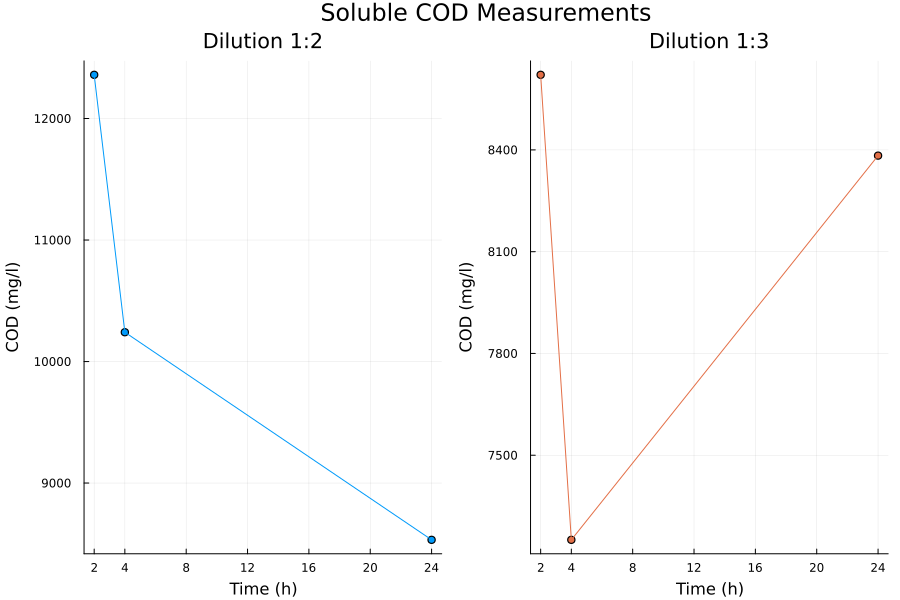
\includegraphics[width=.9\linewidth]{../plots/10_10/COD_plot.png}
\caption{\label{fig:org4983879}Μέτρηση Διαλυτού COD - Δοκιμαστικό Πείραμα 1}
\end{figure}

\item Αρχικό Κινητικό Πείραμα:
\label{sec:orgff164ee}
Το επόμενο πείραμα ήταν το δοκιμαστικό πείραμα κινητικής το οποίο έγινε στους 45 \(^oC\). Από το πείραμα αυτό μετρήθηκαν πολλές διαφορετικές αποκρίσεις για να διαπιστωθεί ποιές έχουν νόημα και ποιές όχι και επίσης έγινε συχνή δειγματοληψία.

Λόγω της πολύ μεγάλης διάρκειας του πειράματος και των συχνών δειγματοληψιών, παρατηρήθηκε πως η στάθμη του δοχείου στα 2 πειράματα μειώθηκε αρκετά (περίπου 550 ml ενώ ξεκίνησε από 800 ml). Η μεγάλη μεταβολή του όγκου, που οφείλεται σε μεγάλο βαθμό στην απώλεια νερού, επηρεάζει μάλλον και τις συγκεντρώσεις που μετρήθηκαν σε κάποιο βαθμό. Για αυτό και αποφασίστηκε η δειγματοληψία να γίνεται μία φορά την ημέρα για τα επόμενα πειράματα.

Συγκεκριμένα, η μέτρηση των ολικών και πτητικών αιωρούμενων στερεών θεωρείται πως δεν είναι αξιόπιστη καθώς παρουσιάζει έντονη παλινδρομική συμπεριφορά ενώ θεωρητικά δεν υπάρχει κάποια εξήγηση για την αύξηση των στερεών (πέρα από να επηρεάστηκαν από την μεταβολή του όγκου του νερού).

Μία αντίστοιχη παλινδρομική συμπεριφορά διαπιστώθηκε και στο \acrshort{cod}. Στην περίπτωση αυτή, παρότι σίγουρα επηρεάζεται και αυτό από τα παραπάνω προβλήματα, είναι πολύ πιο εύκολο να εξηγηθεί η παρουσία ταλαντώσεων. Εφόσον συμβαίνει ταυτόχρονα υδρόλυση και ζύμωση, η μία διεργασία αυξάνει το COD ενώ η άλλη το μειώνει. Οι ρυθμοί αυτοί είναι δυναμικοί καθώς εξαρτώνται από πολλούς παράγοντες. Οπότε, παρόλο που από το \acrshort{cod} μπορεί να καταγραφεί μία ένδειξη του ποιός ρυθμός είναι και ο υψηλότερος την κάθε στιγμή, δεν θεωρείται η πιο καλή ανάλυση για την μελέτη της διεργασίας. Στο Σχήμα \ref{fig:org076c7d0} φαίνονται τα αποτελέσματα της ανάλυσης αυτής.

\begin{figure}[htbp]
\centering
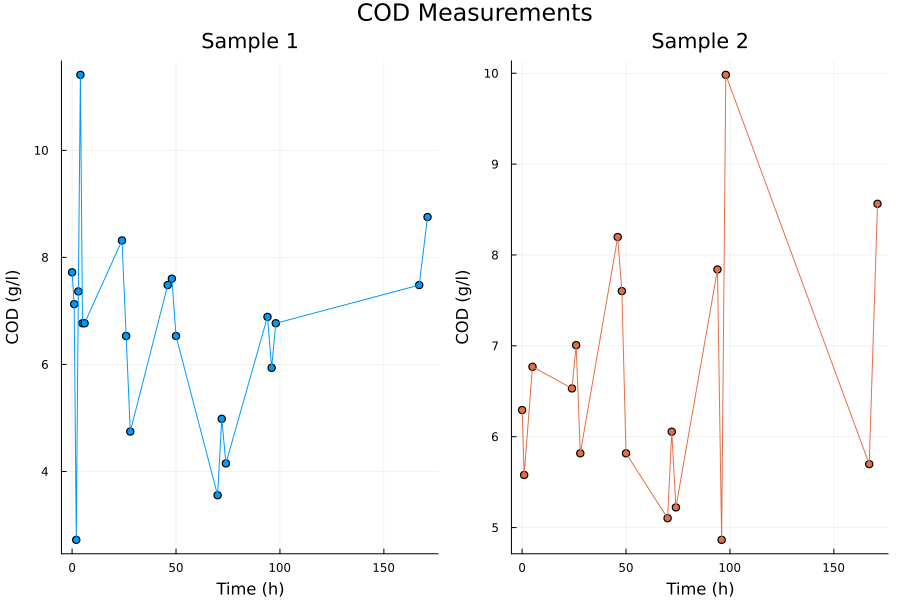
\includegraphics[width=.9\linewidth]{../plots/23_10/cod_scatter_23_10.png}
\caption{\label{fig:org076c7d0}Μέτρηση COD - Αρχικό Κινητικό Πείραμα}
\end{figure}

Λόγω των προβλημάτων της ανάλυσης αυτής, αποφασίστηκε να γίνει μία πιο στοχευμένη ανάλυση. Από την βιβλιογραφία, είναι γνωστό πως η \acrfull{hplc} είναι μία αναλυτική μέθοδος η οποία μπορεί να ανιχνεύσει σάκχαρα, αλκόολες και πτητικά λιπαρά οξέα (\citeprocitem{93}{Zaky et al. 2017}; \citeprocitem{74}{Temudo, Kleerebezem, and van Loosdrecht 2007}; \citeprocitem{24}{Graunke and Wilkie 2014}) . Οπότε, έγινε μία \acrshort{hplc} στα δείγματα των πειραμάτων αυτών για να βγεί ένα καλύτερο συμπέρασμα για την διεργασία. Όπως αναφέρθηκε στην \autoref{sec:analyses}, στα δείγματα του πειράματος αυτού (καθώς και των επόμενων) ταυτοποιήθηκαν οι: γλυκόζη, φρουκτόζη, σακχαρόζη, γαλακτικό οξύ, οξικό οξύ, προπιονικό οξύ και αιθανόλη. Οι ενώσεις αυτές χωρίζονται σε 2 κατηγορίες. Τα σάκχαρα (γλυκόζη, φρουκτόζη, σακχαρόζη) τα οποία παράγονται από την υδρόλυση και καταναλώνονται από την ζύμωση και τα προϊόντα της ζύμωσης (γαλακτικό οξύ, οξικό οξύ, προπιονικό οξύ και αιθανόλη). Παρότι η αιθανόλη δεν είναι οργανικό οξύ, επειδή κατατάσσεται στα προϊόντα της οξεογένεσης, συνήθως λαμβάνεται υπόψην όταν αναφέρονται τα συνολικά \acrfull{vfa}.

Εκτός από ταυτοποίηση των ενώσεων αυτών, η \acrshort{hplc} έχει την δυνατότητα να κάνει ποσοτική ανάλυση, καθώς η επιφάνεια της κάθε κορυφής στο χρωματογράφημα που προκύπτει από την ανάλυση είναι ανάλογη της συγκέντρωσης της ένωσης. Οπότε, με μία καμπύλη βαθμονόμησης, μπορεί να υπολογιστεί η κάθε συγκέντρωση. Επειδή όμως οι επιφάνειες είναι πολύ μεγαλύτερες των συγκεντρώσεων, η καμπύλη πρέπει να γίνει με την μορφή \(\text{Area} = aC + b\) και όχι \(C = a\text{Area} + b\) επειδή στην δεύτερη περίπτωση, οι συντέλεστες της καμπύλης θα τείνουν στο 0, το οποίο θα δημιουργήσει σφάλματα. Στην εξίσωση \ref{eqn:hplc-calibration} φαίνονται οι εξισώσεις βαθμονόμησης για κάθε ένωση.

\begin{subequations}
\label{eqn:hplc-calibration}
\begin{align}
C &= \frac{\text{Area} - 5131.12}{130943.83} & \text{Σακχαρόζη} \label{eqn:hplc-sucrose} \\
C &= \frac{\text{Area} - 7899.51}{264251.52} & \text{Γλυκόζη} \label{eqn:hplc-glucose} \\
C &= \frac{\text{Area} + 11335.7}{270115.2} & \text{Φρουκτόζη} \label{eqn:hplc-fructose} \\
C &= \frac{\text{Area} - 0.946}{1521.642} & \text{Γαλακτικό Οξύ} \label{eqn:hplc-lactate} \\
C &= \frac{\text{Area} + 0.684}{1092.079} & \text{Οξικό Οξύ} \label{eqn:hplc-acetate} \\
C &= \frac{\text{Area} + 25.17}{1060.057} & \text{Προπιονικό Οξύ} \label{eqn:hplc-propionate} \\
C &= \frac{\text{Area} - 8775.42}{113284.075} & \text{Αιθανόλη} \label{eqn:hplc-ethanol}
\end{align}
\end{subequations}

Τα συγκεντρωτικά αποτελέσματα της ανάλυσης αυτής φαίνονται στο Σχήμα \ref{fig:org1a790c4}. 

\begin{figure}[htbp]
\centering
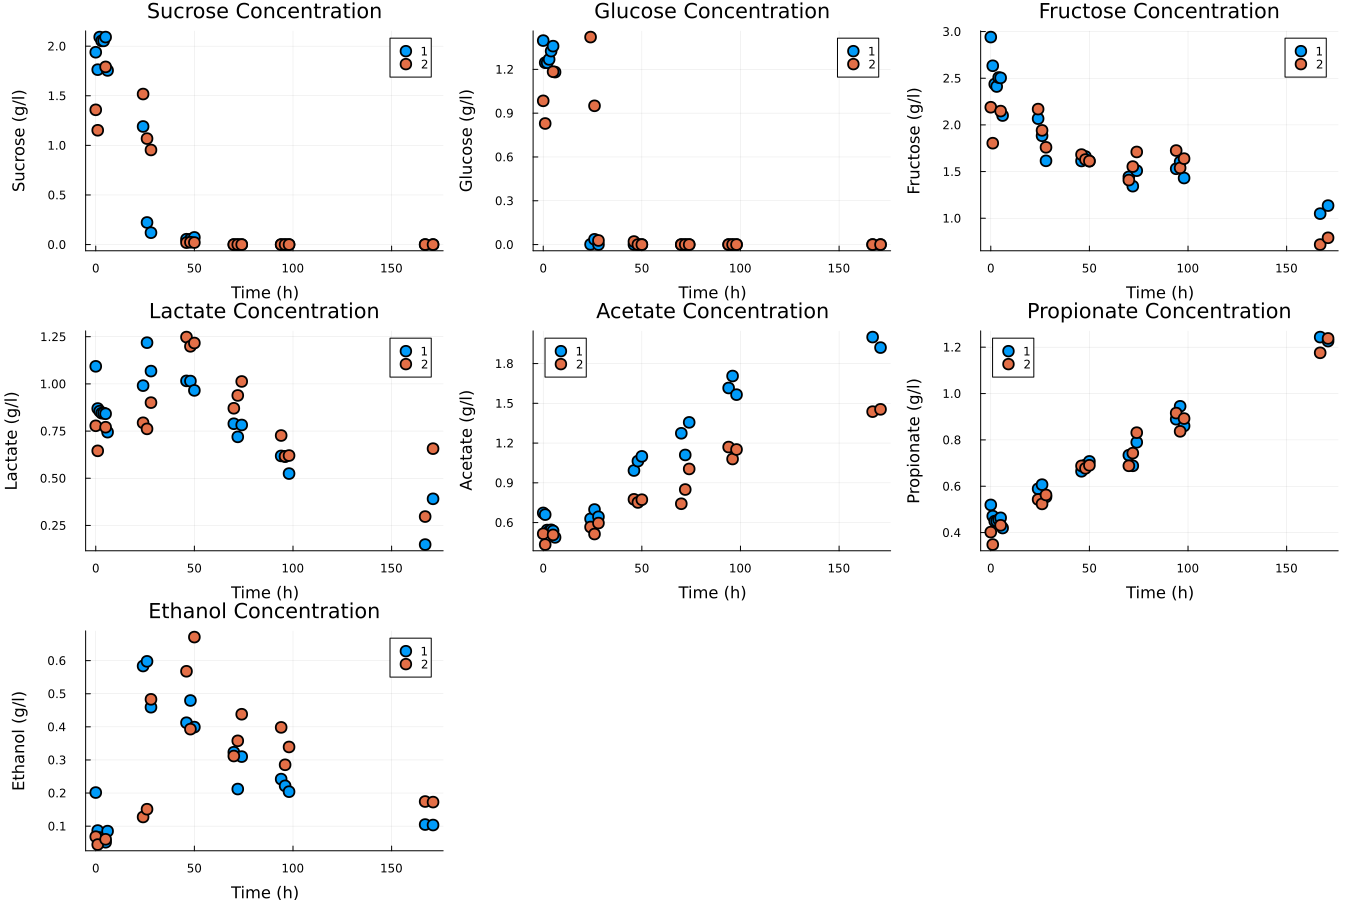
\includegraphics[width=.9\linewidth]{../plots/23_10/final_scatter_23_10.png}
\caption{\label{fig:org1a790c4}Συνολικά Αποτελέσματα HPLC - Αρχικό Κινητικό Πείραμα}
\end{figure}

Δύο ακόμη διαγράμματα που θεωρήθηκαν χρήσιμα ήταν τα συγκεντρωτικά διαγράμματα της συγκέντρωσης σακχάρων () και προϊόντων (\ref{fig:org49ab844}), από τα οποία μπορούν να φανούν περισσότερο κάποιες τάσεις που υπάρχουν στην διεργασία.

\begin{figure}[htbp]
\centering
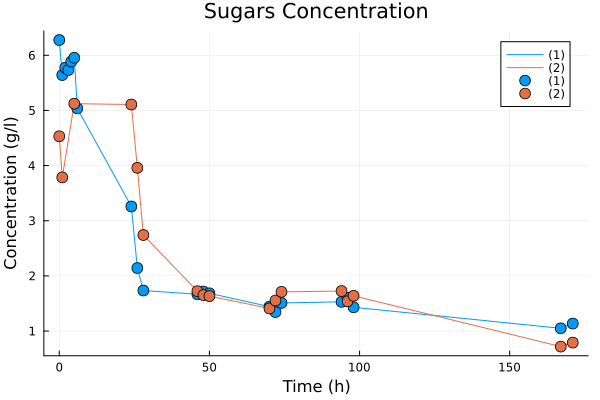
\includegraphics[width=300px]{../plots/23_10/sugars_conc_scatter_23_10.png}
\caption{\label{fig:orgb81b0d6}Συνολική Συγκέντρωση Σακχάρων - Αρχικό Κινητικό Πείραμα}
\end{figure}

\begin{figure}[htbp]
\centering
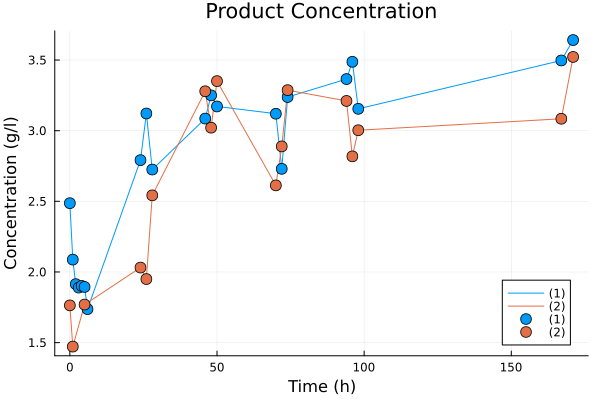
\includegraphics[width=300px]{../plots/23_10/product_conc_scatter_23_10.png}
\caption{\label{fig:org49ab844}Συνολική Συγκέντρωση Προϊόντων - Αρχικό Κινητικό Πείραμα}
\end{figure}

\item Ρυθμός Εξάτμισης Νερού:
\label{sec:org376545b}
Το τελευταίο δοκιμαστικό πείραμα ήταν για την εξάτμιση του νερού. Ο πίνακας \ref{tab:org6ae0b1e} δείχνει τα αποτελέσματα της μείωσης της συνολικής υγρής μάζας καθώς και των \acrshort{ts}, από τα οποία προκύπτει η μείωση της μάζας του νερού.

\begin{table}[htbp]
\caption{\label{tab:org6ae0b1e}Ρυθμός Μεταβολής Υγρής και Ξηρής Μάζας}
\centering
\begin{tabular}{rrrr}
Ημέρα & Μείωση Υγρής Μάζας (g) & Μείωση TS (g) & Εξάτμιση Νερού (g)\\[0pt]
\hline
1 & 6.97 & 1.68 & 5.28\\[0pt]
2 & 12.88 & 2.35 & 10.53\\[0pt]
3 & 15.68 & -0.73 & 16.42\\[0pt]
7 & 36.23 & 5.22 & 31.01\\[0pt]
9 & 38.06 & 3.83 & 34.23\\[0pt]
11 & 44.74 & 5.47 & 39.27\\[0pt]
14 & 45.49 & 7.86 & 37.63\\[0pt]
\end{tabular}
\end{table}

Από τα αποτελέσματα αυτά, παρατηρείται πως η υγρή μάζα αρχικά μειώνεται γρήγορα και μεταξύ 11 και 14 ημέρων έχει φτάσει ένα πλατό. Ο ρυθμός εξάτμισης του νερού φαίνεται να έχει παρόμοια τάση, βέβαια την τελευταία ημέρα που έγινε δειγματοληψία, η εξάτμιση μειώθηκε. Τα ευρήματα αυτά οδηγούν στην θεώρηση ότι ο ρυθμός εξάτμισης μπορεί να περιγραφεί πολύ καλά με μία παραβολική εξίσωση. Κάνοντας την προσαρμογή, προκύπτει πως για το πείραμα αυτό, το οποίο διεξάχθηκε στους 35 \(^oC\), ο ρυθμός εξάτμισης δίνεται από την εξίσωση

\[ \text{Evaporation Rate} = -0.252t^2 + 6.287t - 0.723 ~ ~ ~ R^2 = 0.997 \]

με τον χρόνο να είναι εκφρασμένος σε ημέρες.

Για την μείωση των TS δεν μπορεί να προκύψει κάποιο ικανοποιητικό συμπέρασμα, το οποίο συνάδει με τις παρατηρήσεις των άλλων δοκιμαστικών πειραμάτων που έκριναν τα στερεά μη ικανοποιητικά για την παρακολούθηση της υδρόλυσης.
\end{enumerate}

\section{Βασικός πειραματικός κύκλος υδρόλυσης εργαστηριακής κλίμακας}
\label{sec:org9858883}
Για τον βασικό πειραματικό κύκλο της υδρόλυσης, έγιναν 2 πειράματα στα οποία εξετάστηκε η υδρόλυση 5 διαφορετικών αναλογιών \acrshort{mix}/\acrshort{fw}. Οι αναλογίες ήταν 0, 1, 2, 4 και 8 mL \acrshort{mix} ανά 200 g \acrshort{fw}. Η θερμοκρασία ρυθμίστηκε στους 35 \(^oC\) για το πρώτο πείραμα και στους 40 \(^oC\) για το δεύτερο, όπως αναφέρθηκε και στην \autoref{sec:lab-hydro}. Τα πρωτογενή πειραματικά αποτελέσματα ήταν αρχικό και τελικό COD καθώς και τα αποτελέσματα της HPLC όπως και για το αρχικό κινητικό πείραμα, ενώ τα δευτερογενή συγκριτικά αποτελέσματα μεταξύ των κύκλων θα παρουσιαστούν στο \autoref{sec:result_discussion} στα πλαίσια της συζήτησης των αποτελεσμάτων για να αποφανθούν οι βέλτιστες λειτουργικές συνθήκες.

\begin{enumerate}
\item Πείραμα στους 35 \(^oC\):
\label{sec:org21736ec}
Η μεταβολή του \acrshort{cod} κατά τις 72 ώρες ταυτόχρονης υδρόλυσης και ζύμωσης φαίνεται στο Σχήμα \ref{fig:org2313470}.

\begin{figure}[htbp]
\centering
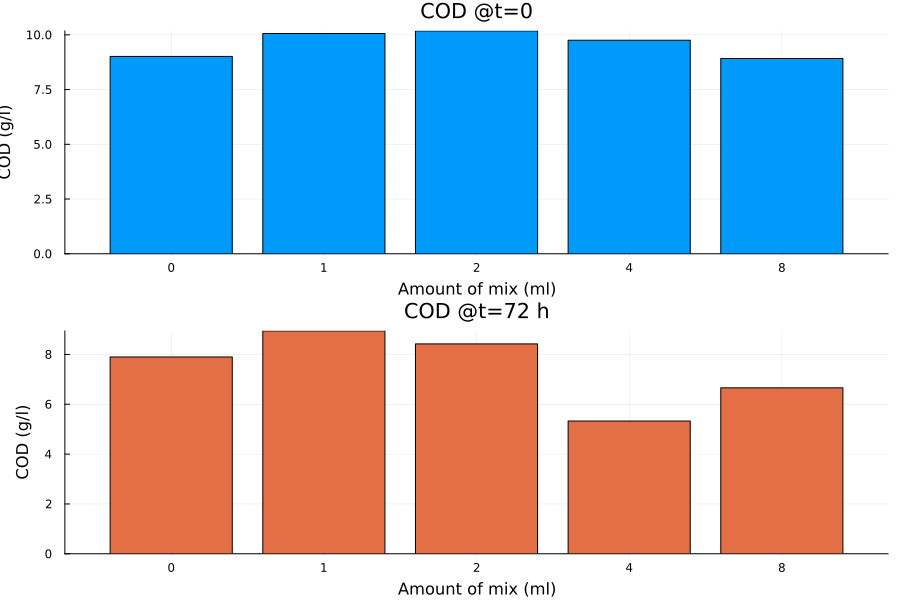
\includegraphics[width=.9\linewidth]{../plots/10_11/cod_bar_10_11.png}
\caption{\label{fig:org2313470}Μεταβολή του COD κατά την υδρόλυση/ζύμωση - Πείραμα 35 \(^oC\)}
\end{figure}

Από την μεταβολή του \acrshort{cod} φαίνεται πως γενικά υπάρχει μία μείωση κατά την διεργασία, το οποίο συμφωνεί και με τα αποτελέσματα των δοκιμαστικών πειραμάτων. Επίσης, φαίνεται πως όσο περισσότερο \acrshort{mix} προστίθεται, η μείωση του \acrshort{cod} γίνεται όλο και περισσότερη (με μοναδική εξαίρεση πως το 8 mL έχει μικρότερη μείωση από το 4). (εδώ ίσως να βάλω groupedbars για το plot). Αυτό εξηγείται, καθώς όσο προστίθεται το \acrshort{mix} προστίθενται ενεργοί μικροοργανισμοί, οι οποίοι όχι μόνο υδρολύουν το υπόστρωμα, αλλά καταναλώνουν και κάποια ποσότητα από το \acrfull{scod}.

Τα συγκεντρωτικά αποτελέσματα της HPLC φαίνονται στο Σχήμα \ref{fig:org99252a8}. Εκτός από τα αποτελέσματα αυτά, το διάγραμμα περιέχει και την μέτρηση του pH, η οποία είχε γίνει στο πείραμα αυτό. Θέλω να αντικαταστήσω το διάγραμμα με ένα scatter με γραμμές αλλά δεν το έχω έτοιμο.

\begin{figure}[htbp]
\centering
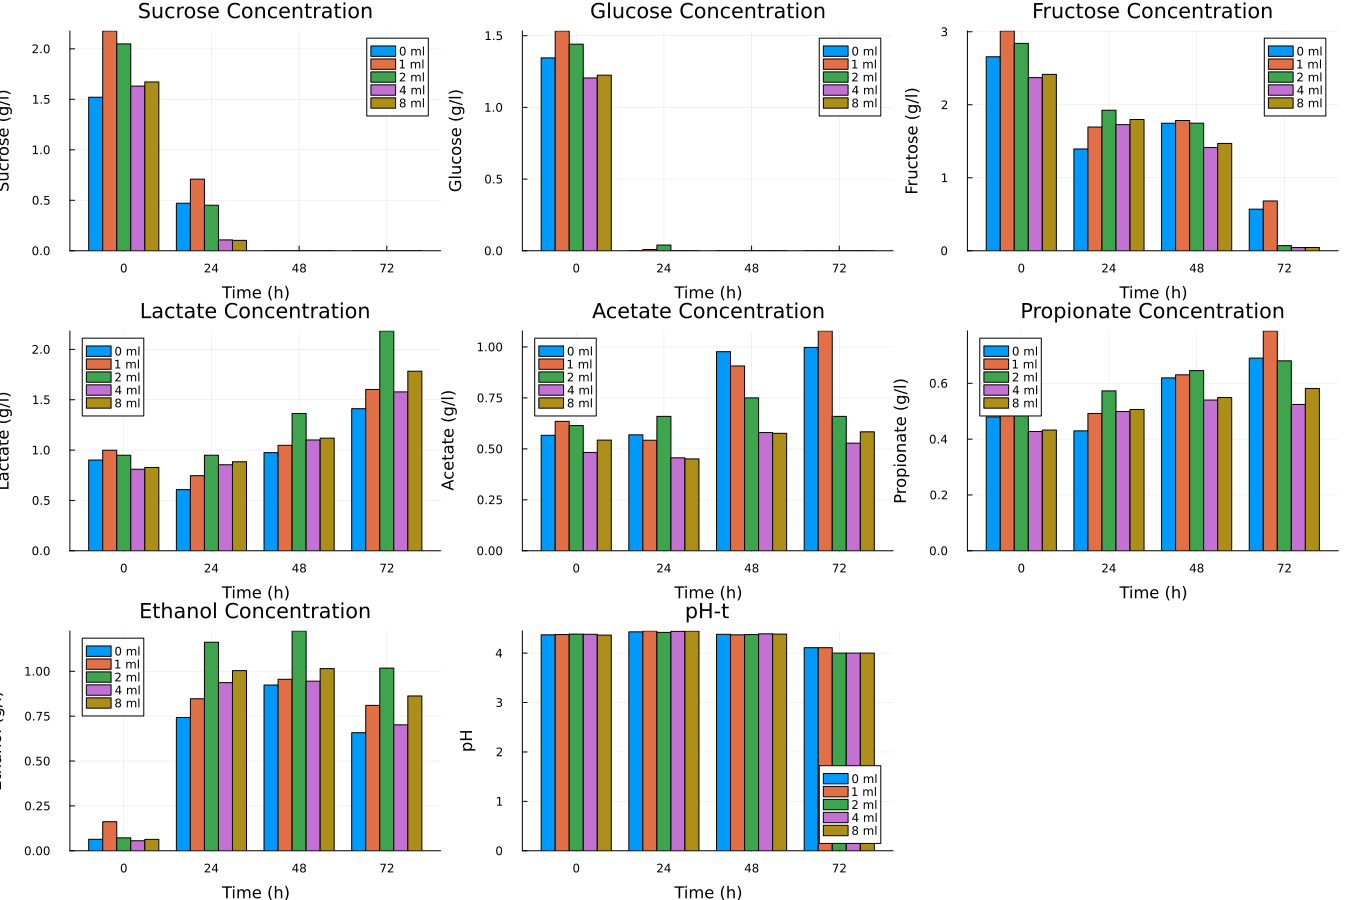
\includegraphics[width=.9\linewidth]{../plots/10_11/final_bar_10_11.png}
\caption{\label{fig:org99252a8}Συνολικά Αποτελέσματα HPLC - Πείραμα 35 \(^oC\)}
\end{figure}

Επίσης παρουσιάζονται τα συγκεντρωτικά διαγράμματα σακχάρων και προϊόντων όπως έγινε και για το αρχικό κινητικό πείραμα. 

\begin{figure}[htbp]
\centering
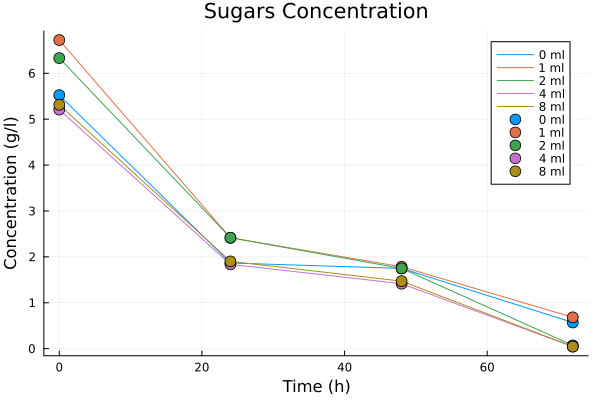
\includegraphics[width=300px]{../plots/10_11/sugars_conc_scatter_10_11.png}
\caption{\label{fig:orgfd6671c}Συνολική Συγκέντρωση Σακχάρων - Πείραμα 35 \(^oC\)}
\end{figure}

\begin{figure}[htbp]
\centering
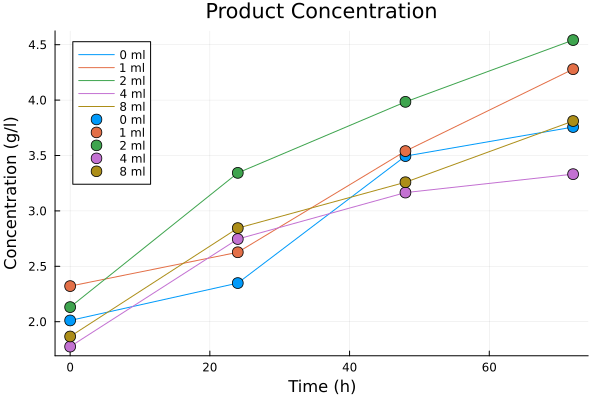
\includegraphics[width=300px]{../plots/10_11/product_conc_scatter_10_11.png}
\caption{\label{fig:org024ea48}Συνολική Συγκέντρωση Προϊόντων - Πείραμα 35 \(^oC\)}
\end{figure}

\item Πείραμα στους 40 \(^oC\)
\label{sec:org76c5c5c}
Τα αντίστοιχα αποτελέσματα προέκυψαν και από αυτό το πείραμα. Στο Σχήμα φαίνεται η μεταβολή του \acrshort{scod} κατά την διάρκεια της υδρόλυσης/ζύμωσης.

\begin{center}
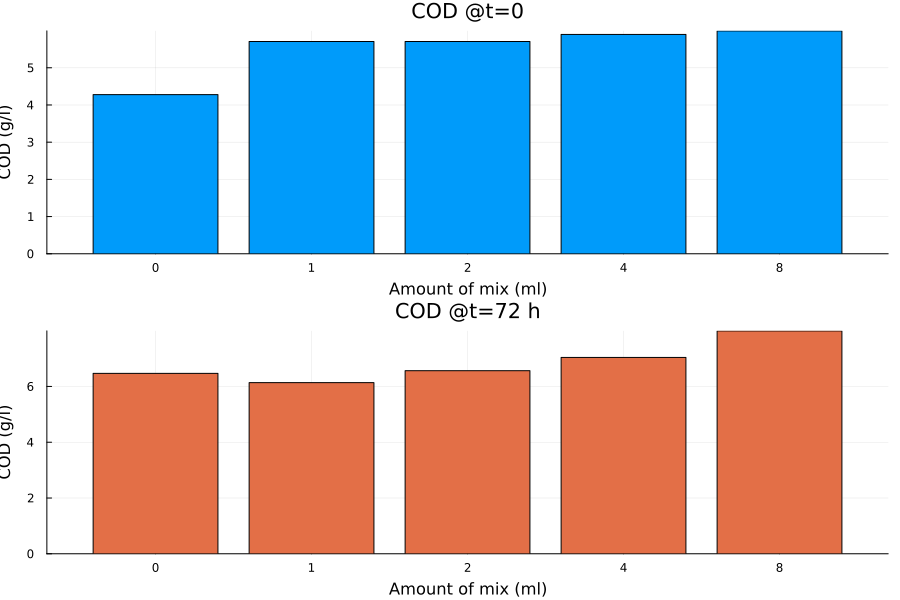
\includegraphics[width=.9\linewidth]{../plots/28_11/cod_bar_28_11.png}
\end{center}

Στο πείραμα αυτό, παρατηρείται μία τάση σχετικά διαφορετική από τα προηγούμενα πειράματα, καθώς το \acrshort{cod} γενικά αυξάνεται με την ζύμωση. Η πιο πιθανή εξήγηση είναι πως το αρχικό \acrshort{cod} ήταν πολύ χαμηλό, οπότε η υδρόλυση είχε γρηγορότερο ρυθμό από την ζύμωση γενικότερα και ως αποτέλεσμα φαίνεται περισσότερο η αύξηση.

Τα αποτελέσματα της HPLC φαίνονται στα Σχήματα \ref{fig:org977d4ed}, \ref{fig:org1affc46} και \ref{fig:org754ce98}.

\begin{figure}[htbp]
\centering
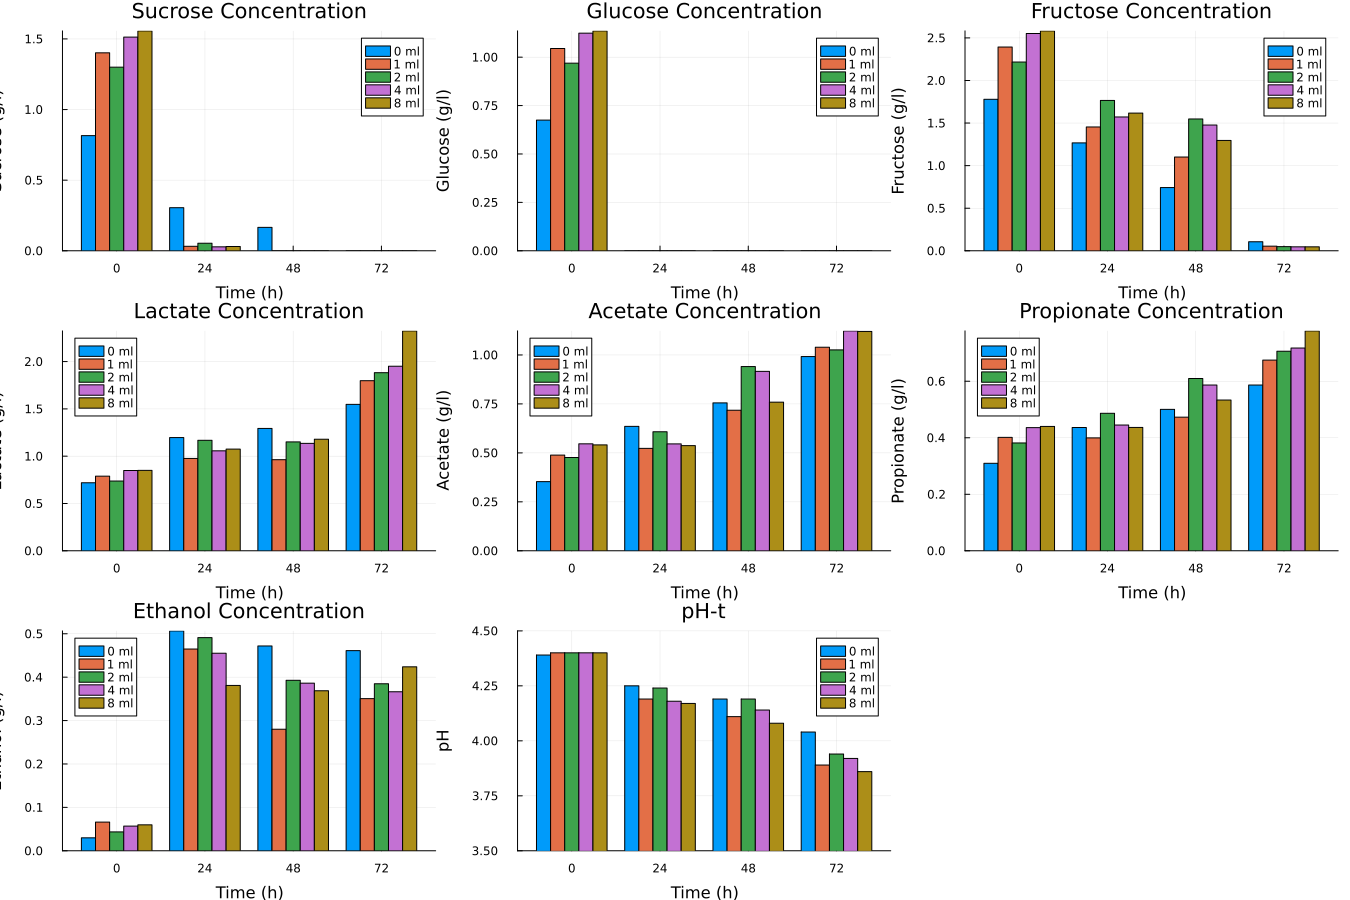
\includegraphics[width=.9\linewidth]{../plots/28_11/final_bar_28_11.png}
\caption{\label{fig:org977d4ed}Συνολικά Αποτελέσματα HPLC - Πείραμα 40 \(^oC\)}
\end{figure}

\begin{figure}[htbp]
\centering
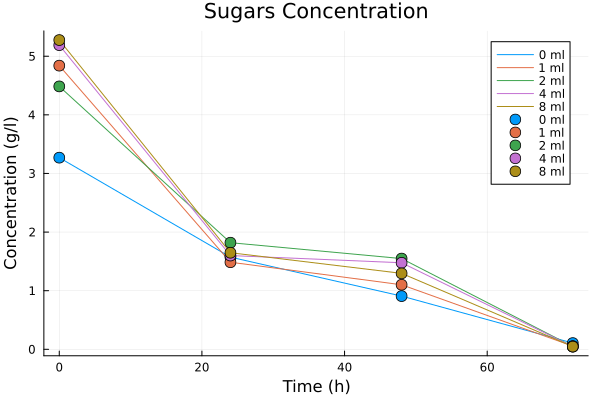
\includegraphics[width=300px]{../plots/28_11/sugars_conc_scatter_28_11.png}
\caption{\label{fig:org1affc46}Συνολική Συγκέντρωση Σακχάρων - Πείραμα 40 \(^oC\)}
\end{figure}

\begin{figure}[htbp]
\centering
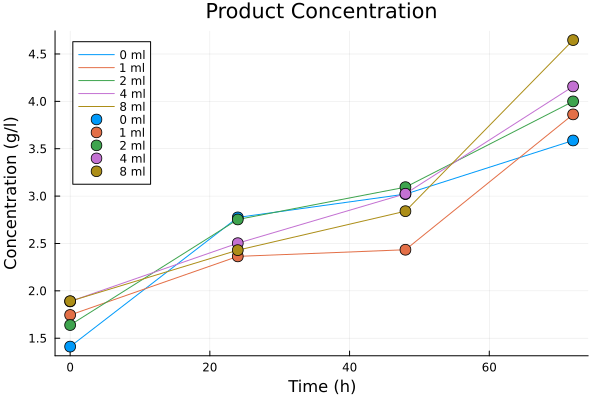
\includegraphics[width=300px]{../plots/28_11/product_conc_scatter_28_11.png}
\caption{\label{fig:org754ce98}Συνολική Συγκέντρωση Προϊόντων - Πείραμα 40 \(^oC\)}
\end{figure}
\end{enumerate}

\section{Πειράματα υδρόλυσης πιλοτικής κλίμακας}
\label{sec:orgdf5ab29}
Στην πιλοτική κλίμακα έγιναν 3 πειράματα υδρόλυσης, οι συνθήκες των οποίων φαίνονται στην \autoref{sec:pilot-exp} . Παρακάτω, φαίνονται τα στερεά και το \acrshort{cod} για το κάθε πείραμα. Αξίζει να σημειωθεί πως η καθημερινή τροφοδοσία στο όργανο αυτό δεν είναι ίδια, καθώς τα υπολείμματα τροφών που συλλέγονται από ένα εστιατόριο έχουν εκ φύσεων ανομοιογένεια από μέρα σε μέρα. Οπότε, μπορούν να παρατηρηθούν αποκλίσεις που οφείλονται σε αυτό στα παρακάτω αποτελέσματα. Για τον λόγο αυτόν, ως υπόστρωμα στην αναερόβια χώνευση χρησιμοποιήθηκε μία υγρή απορροή που αποτελείται από μίγμα των απορροών των 4 ημερών και περιγράφεται από τον μέσο όρο και την τυπική απόκλιση που φαίνονται σε κάθε πίνακα. Η τυπική απόκλιση αυτή είναι και ένα μέτρο του πόσο σφάλμα αναμένεται να υπάρχει λόγω της ανομοιογένειας στην τροφοδοσία.

\begin{table}[htbp]
\caption{\label{tab:org4b5c81f}Υδρόλυση Πιλοτικής Κλίμακας - Πρώτος Κύκλος}
\centering
\begin{tabular}{rrrrrrr}
Day & TS (\(\%\)) & VS (\(\%\)) & VS/TS (\(\%\)) & sCOD (mg/L) & tCOD (mg/L) & sCOD/tCOD (\(\%\))\\[0pt]
\hline
1 & 0.63 & 0.54 & 86.08 & 4561.5 & 8792.7 & 51.88\\[0pt]
2 & 1.26 & 1.17 & 92.64 & 8135.1 & 13077.5 & 62.21\\[0pt]
3 & 2.54 & 2.48 & 97.38 & 11134.4 & 37476.6 & 29.71\\[0pt]
4 & 2.47 & 2.42 & 97.79 & 12991.1 & 32053.8 & 40.53\\[0pt]
 &  &  &  &  &  & \\[0pt]
Mean & 1.73 & 1.65 & 93.47 & 9205.5 & 22850.2 & 46.08\\[0pt]
StDev & 0.81 & 0.83 & 4.73 & 3192.3 & 12163.0 & 12.17\\[0pt]
\end{tabular}
\end{table}

\begin{table}[htbp]
\caption{\label{tab:orgd6d9eb3}Υδρόλυση Πιλοτικής Κλίμακας - Δεύτερος Κύκλος}
\centering
\begin{tabular}{rrrrrrr}
Day & TS (\(\%\)) & VS (\(\%\)) & VS/TS (\(\%\)) & sCOD (mg/L) & tCOD (mg/L) & sCOD/tCOD (\(\%\))\\[0pt]
\hline
1 & 1.07 & 0.97 & 91.05 & 6659.2 & 14029.6 & 47.47\\[0pt]
2 & 0.62 & 0.51 & 82.13 & 4754.9 & 9387.8 & 50.65\\[0pt]
3 & 0.59 & 0.50 & 85.67 & 3088.6 & 9149.8 & 33.76\\[0pt]
4 & 1.54 & 1.48 & 96.28 & 5421.4 & 21699.1 & 24.98\\[0pt]
 &  &  &  &  &  & \\[0pt]
Mean & 0.95 & 0.87 & 88.78 & 4981.0 & 13566.6 & 39.21\\[0pt]
StDev & 0.39 & 0.40 & 0.40 & 1288.7 & 5082.4 & 10.38\\[0pt]
\end{tabular}
\end{table}

\begin{table}[htbp]
\caption{\label{tab:org41c4e9d}Υδρόλυση Πιλοτικής Κλίμακας - Τρίτος Κύκλος}
\centering
\begin{tabular}{rrrrrrr}
Day & TS (\(\%\)) & VS ($\backslash$\(\%\)) & VS/TS (\(\%\)) & sCOD (mg/L) & tCOD (mg/L) & sCOD/tCOD (\(\%\))\\[0pt]
\hline
1 & 1.10 & 1.05 & 95.01 & 6326.0 & 13791.6 & 45.87\\[0pt]
2 & 0.65 & 0.59 & 91.55 & 2326.9 & 7781.1 & 29.90\\[0pt]
3 & 0.57 & 0.52 & 89.81 & 1184.3 & 6650.4 & 17.81\\[0pt]
4 & 1.00 & 0.92 & 92.29 & 4600.2 & 12333.8 & 37.30\\[0pt]
 &  &  &  &  &  & \\[0pt]
Mean & 0.83 & 0.77 & 92.16 & 3609.3 & 10139.2 & 32.72\\[0pt]
StDev & 0.22 & 0.22 & 1.87 & 1993.0 & 2995.4 & 10.30\\[0pt]
\end{tabular}
\end{table}

\section{Πειράματα αναερόβιας χώνευσης}
\label{sec:org16e88db}

\begin{enumerate}
\item ΑΧ εργαστηριακών υδρολυμάτων με Λάσπη 1:
\label{sec:org0076b27}

\item ΑΧ εργαστηριακών υδρολυμάτων με Λάσπη 2:
\label{sec:orgedf64f4}

\item AX πιλοτικών υδρολυμάτων:
\label{sec:org9911879}
\end{enumerate}

\chapter{Συζήτηση Αποτελεσμάτων}
\label{sec:orgfef721f}
\label{sec:result_discussion}

\chapter{Συμπεράσματα και Προτάσεις}
\label{sec:org632b076}
\label{sec:conclusion}

\part*{Βιβλιογραφία}
\label{sec:orgba39742}
\begin{hangparas}{1.5em}{1}
\hypertarget{citeproc_bib_item_1}{Anwar Saeed, Mashair, Hongzhi Ma, Siyuan Yue, Qunhui Wang, and Maobing Tu. 2018. “Concise Review on Ethanol Production from Food Waste: Development and Sustainability.” \textit{Environmental Science and Pollution Research} 25 (29): 28851–63. \url{https://doi.org/10.1007/s11356-018-2972-4}.}

\hypertarget{citeproc_bib_item_2}{APHA, AWWA, and WEF. 2005. \textit{Standard Methods for the Examination of Water and Wastewater}. 24th ed. APHA, AWWA, WEF.}

\hypertarget{citeproc_bib_item_3}{Arora, Sidharth, Richa Rani, and Sanjoy Ghosh. 2018. “Bioreactors in Solid State Fermentation Technology: Design, Applications and Engineering Aspects.” \textit{Journal of Biotechnology} 269 (March): 16–34. \url{https://doi.org/10.1016/j.jbiotec.2018.01.010}.}

\hypertarget{citeproc_bib_item_4}{Azbar, Nuri, Pepi Ursillo, and Richard E. Speece. 2001. “Effect of Process Configuration and Substrate Complexity on the Performance of Anaerobic Processes.” \textit{Water Research} 35 (3): 817–29. \url{https://doi.org/10.1016/S0043-1354(00)00318-3}.}

\hypertarget{citeproc_bib_item_5}{Bezanson, Jeff, Alan Edelman, Stefan Karpinski, and Viral B Shah. 2017. “Julia: A Fresh Approach to Numerical Computing.” \textit{Siam Review} 59 (1): 65–98. \url{https://doi.org/10.1137/141000671}.}

\hypertarget{citeproc_bib_item_6}{Bouchet-Valat, Milan, and Bogumił Kamiński. 2023. “Dataframes.Jl: Flexible and Fast Tabular Data in Julia.” \textit{Journal of Statistical Software} 107 (4): 1–32. \url{https://doi.org/10.18637/jss.v107.i04}.}

\hypertarget{citeproc_bib_item_7}{Canul Bacab, Fernando, Elda España Gamboa, Juan Enrique Ruiz Espinoza, Rosa M. Leal-Bautista, Raúl Tapia Tussell, Jorge Domínguez Maldonado, Blondy Canto Canché, and Liliana Alzate-Gaviria. 2020. “Two Phase Anaerobic Digestion System of Municipal Solid Waste by Utilizing Microaeration and Granular Activated Carbon.” \textit{Energies} 13 (4): 933. \url{https://doi.org/10.3390/en13040933}.}

\hypertarget{citeproc_bib_item_8}{Cekmecelioglu, Deniz, and Oya N. Uncu. 2013. “Kinetic Modeling of Enzymatic Hydrolysis of Pretreated Kitchen Wastes for Enhancing Bioethanol Production.” \textit{Waste Management} 33 (3): 735–39. \url{https://doi.org/10.1016/j.wasman.2012.08.003}.}

\hypertarget{citeproc_bib_item_9}{Cerda, A., A. Artola, X. Font, R. Barrena, T. Gea, and A. Sánchez. 2018. “Composting of Food Wastes: Status and Challenges.” \textit{Bioresource Technology} 248: 57–67. \url{https://doi.org/10.1016/j.biortech.2017.06.133}.}

\hypertarget{citeproc_bib_item_10}{Cesaro, Alessandra, and Vincenzo Belgiorno. 2014. “Pretreatment Methods to Improve Anaerobic Biodegradability of Organic Municipal Solid Waste Fractions.” \textit{Chemical Engineering Journal} 240 (March): 24–37. \url{https://doi.org/10.1016/j.cej.2013.11.055}.}

\hypertarget{citeproc_bib_item_11}{Cheng, Jun, Junjie Hua, Ting Kang, Bo Meng, Liangchen Yue, Haiquan Dong, Hui Li, and Junhu Zhou. 2020. “Nanoscale Zero-Valent Iron Improved Lactic Acid Degradation to Produce Methane through Anaerobic Digestion.” \textit{Bioresource Technology} 317 (December): 124013. \url{https://doi.org/10.1016/j.biortech.2020.124013}.}

\hypertarget{citeproc_bib_item_12}{Chen, Qing, Wanqing Wu, Dacheng Qi, Yihong Ding, and Zihao Zhao. 2020. “Review on Microaeration-Based Anaerobic Digestion: State of the Art, Challenges, and Prospectives.” \textit{Science of the Total Environment} 710 (March): 136388. \url{https://doi.org/10.1016/j.scitotenv.2019.136388}.}

\hypertarget{citeproc_bib_item_13}{Chen, Xikai, Xietian Zheng, Yanbo Pei, Weikun Chen, Qiang Lin, Jingang Huang, Pingzhi Hou, Junhong Tang, and Wei Han. 2022. “Process Design and Techno-Economic Analysis of Fuel Ethanol Production from Food Waste by Enzymatic Hydrolysis and Fermentation.” \textit{Bioresource Technology} 363 (November): 127882. \url{https://doi.org/10.1016/j.biortech.2022.127882}.}

\hypertarget{citeproc_bib_item_14}{Chen, Xue, Hairong Yuan, Dexun Zou, Yanping Liu, Baoning Zhu, Akiber Chufo, Muhammad Jaffar, and Xiujin Li. 2015. “Improving Biomethane Yield by Controlling Fermentation Type of Acidogenic Phase in Two-Phase Anaerobic Co-Digestion of Food Waste and Rice Straw.” \textit{Chemical Engineering Journal} 273 (August): 254–60. \url{https://doi.org/10.1016/j.cej.2015.03.067}.}

\hypertarget{citeproc_bib_item_15}{Christ, Simon, Daniel Schwabeneder, Christopher Rackauckas, Michael Krabbe Borregaard, and Thomas Breloff. 2023. “Plots.Jl – a User Extendable Plotting Api for the Julia Programming Language.” \url{https://doi.org/https://doi.org/10.5334/jors.431}.}

\hypertarget{citeproc_bib_item_16}{Dai, Kun, Jun-Li Wen, Fang Zhang, and Raymond Zeng. 2017. “Valuable Biochemical Production in Mixed Culture Fermentation: Fundamentals and Process Coupling.” \textit{Applied Microbiology and Biotechnology} 101 (September). \url{https://doi.org/10.1007/s00253-017-8441-z}.}

\hypertarget{citeproc_bib_item_17}{Danisch, Simon, and Julius Krumbiegel. 2021. “Makie.jl: Flexible High-Performance Data Visualization for Julia.” \textit{Journal of Open Source Software} 6 (65): 3349. \url{https://doi.org/10.21105/joss.03349}.}

\hypertarget{citeproc_bib_item_18}{Datseris, George, Jonas Isensee, Sebastian Pech, and Tamás Gál. 2020. “Drwatson: The Perfect Sidekick for Your Scientific Inquiries.” \textit{Journal of Open Source Software} 5 (54): 2673. \url{https://doi.org/10.21105/joss.02673}.}

\hypertarget{citeproc_bib_item_19}{Dhar, Bipro Ranjan, George Nakhla, and Madhumita B. Ray. 2012. “Techno-Economic Evaluation of Ultrasound and Thermal Pretreatments for Enhanced Anaerobic Digestion of Municipal Waste Activated Sludge.” \textit{Waste Management} 32 (3): 542–49. \url{https://doi.org/10.1016/j.wasman.2011.10.007}.}

\hypertarget{citeproc_bib_item_20}{Fang, Hongli, Yongsen Shi, Dunjie Li, Liuying Song, Yu-You Li, Rutao Liu, Dong Yuan, and Qigui Niu. 2020. “Synergistic Co-Digestion of Waste Commercial Yeast and Chicken Manure: Kinetic Simulation, DOM Variation and Microbial Community Assessment.” \textit{Renewable Energy} 162 (December): 2272–84. \url{https://doi.org/10.1016/j.renene.2020.10.038}.}

\hypertarget{citeproc_bib_item_21}{Feng, Kai, Huan Li, and Chengzhi Zheng. 2018. “Shifting Product Spectrum by pH Adjustment during Long-Term Continuous Anaerobic Fermentation of Food Waste.” \textit{Bioresource Technology} 270 (December): 180–88. \url{https://doi.org/10.1016/j.biortech.2018.09.035}.}

\hypertarget{citeproc_bib_item_22}{Feng, Kai, Huan Li, Zhou Deng, Qiao Wang, Yangyang Zhang, and Chengzhi Zheng. 2020. “Effect of Pre-Fermentation Types on the Potential of Methane Production and Energy Recovery from Food Waste.” \textit{Renewable Energy} 146 (February): 1588–95. \url{https://doi.org/10.1016/j.renene.2019.07.127}.}

\hypertarget{citeproc_bib_item_23}{Franchetti, Matthew. 2013. “Economic and Environmental Analysis of Four Different Configurations of Anaerobic Digestion for Food Waste to Energy Conversion Using LCA for: A Food Service Provider Case Study.” \textit{Journal of Environmental Management} 123 (July): 42–48. \url{https://doi.org/10.1016/j.jenvman.2013.03.003}.}

\hypertarget{citeproc_bib_item_24}{Graunke, Ryan E., and Ann C. Wilkie. 2014. “Examining the Mechanisms of Short-Term Solubilization of Ground Food Waste for High-Rate Anaerobic Digestion.” \textit{International Biodeterioration \& Biodegradation} 86 (January): 327–33. \url{https://doi.org/10.1016/j.ibiod.2013.10.007}.}

\hypertarget{citeproc_bib_item_25}{Grippi, Donatella, Rafael Clemente, and Maria Bernal. 2020. “Chemical and Bioenergetic Characterization of Biofuels from Plant Biomass: Perspectives for Southern Europe.” \textit{Applied Sciences} 10 (May): 3571. \url{https://doi.org/10.3390/app10103571}.}

\hypertarget{citeproc_bib_item_26}{Han, Wei, Yingting Yan, Yiwen Shi, Jingjing Gu, Junhong Tang, and Hongting Zhao. 2016. “Biohydrogen Production from Enzymatic Hydrolysis of Food Waste in Batch and Continuous Systems.” \textit{Scientific Reports} 6 (1): 38395. \url{https://doi.org/10.1038/srep38395}.}

\hypertarget{citeproc_bib_item_27}{Hobbs, S.R., A.E. Landis, B.E. Rittmann, M.N. Young, and P. Parameswaran. 2018. “Enhancing Anaerobic Digestion of Food Waste through Biochemical Methane Potential Assays at Different Substrate: Inoculum Ratios.” \textit{Waste Management} 71: 612–17. \url{https://doi.org/10.1016/j.wasman.2017.06.029}.}

\hypertarget{citeproc_bib_item_28}{Infurna, Giulia, Gabriele Caruso, and Nadka Tz Dintcheva. 2023. “Sustainable Materials Containing Biochar Particles: A Review.” \textit{Polymers} 15 (2): 343. \url{https://doi.org/10.3390/polym15020343}.}

\hypertarget{citeproc_bib_item_29}{Ishangulyyev, Rovshen, Sanghyo Kim, and Sang Hyeon Lee. 2019. “Understanding Food Loss and Waste–-Why Are We Losing and Wasting Food?” \textit{Foods} 8 (8): 297. \url{https://doi.org/10.3390/foods8080297}.}

\hypertarget{citeproc_bib_item_30}{Jiang, Jianguo, Yujing Zhang, Kaimin Li, Quan Wang, Changxiu Gong, and Menglu Li. 2013. “Volatile Fatty Acids Production from Food Waste: Effects of pH, Temperature, and Organic Loading Rate.” \textit{Bioresource Technology} 143 (September): 525–30. \url{https://doi.org/10.1016/j.biortech.2013.06.025}.}

\hypertarget{citeproc_bib_item_31}{Jiang, X., Z. Zhao, and Y. Zhang. 2022. “Towards Engineering Application: Integrating Current Strategies of Promoting Direct Interspecies Electron Transfer to Enhance Anaerobic Digestion.” \textit{Chemical Engineering Journal Advances} 12. \url{https://doi.org/10.1016/j.ceja.2022.100405}.}

\hypertarget{citeproc_bib_item_32}{Jing, Y., F. Li, Y. Li, P. Jin, S. Zhu, C. He, J. Zhao, Z. Zhang, and Q. Zhang. 2020. “Statistical Optimization of Simultaneous Saccharification Fermentative Hydrogen Production from Corn Stover.” \textit{Bioengineered} 11 (1): 428–38. \url{https://doi.org/10.1080/21655979.2020.1739405}.}

\hypertarget{citeproc_bib_item_33}{Kavitha, S., J. Rajesh Banu, A. Arul Priya, Do Khac Uan, and Ick Tae Yeom. 2017. “Liquefaction of Food Waste and Its Impacts on Anaerobic Biodegradability, Energy Ratio and Economic Feasibility.” \textit{Applied Energy} 208 (December): 228–38. \url{https://doi.org/10.1016/j.apenergy.2017.10.049}.}

\hypertarget{citeproc_bib_item_34}{Khadka, A., A. Parajuli, S. Dangol, B. Thapa, L. Sapkota, A.A. Carmona-Martínez, and A. Ghimire. 2022. “Effect of the Substrate to Inoculum Ratios on the Kinetics of Biogas Production during the Mesophilic Anaerobic Digestion of Food Waste.” \textit{Energies} 15 (3). \url{https://doi.org/10.3390/en15030834}.}

\hypertarget{citeproc_bib_item_35}{Kim, Dong-Hoon, and Mi-Sun Kim. 2013. “Development of a Novel Three-Stage Fermentation System Converting Food Waste to Hydrogen and Methane.” \textit{Bioresource Technology} 127 (January): 267–74. \url{https://doi.org/10.1016/j.biortech.2012.09.088}.}

\hypertarget{citeproc_bib_item_36}{Kohn, Richard, and Raymond Boston. 2000. “The Role of Thermodynamics in Controlling Rumen Metabolism,” January.}

\hypertarget{citeproc_bib_item_37}{Li, Lei, Qin He, Yao Ma, Xiaoming Wang, and Xuya Peng. 2015. “Dynamics of Microbial Community in a Mesophilic Anaerobic Digester Treating Food Waste: Relationship between Community Structure and Process Stability.” \textit{Bioresource Technology} 189 (August): 113–20. \url{https://doi.org/10.1016/j.biortech.2015.04.015}.}

\hypertarget{citeproc_bib_item_38}{Lim, Jun Wei, and Jing-Yuan Wang. 2013. “Enhanced Hydrolysis and Methane Yield by Applying Microaeration Pretreatment to the Anaerobic Co-Digestion of Brown Water and Food Waste.” \textit{Waste Management} 33 (4): 813–19. \url{https://doi.org/10.1016/j.wasman.2012.11.013}.}

\hypertarget{citeproc_bib_item_39}{Lim, Jun Wei, Jun An Chiam, and Jing-Yuan Wang. 2014. “Microbial Community Structure Reveals How Microaeration Improves Fermentation during Anaerobic Co-Digestion of Brown Water and Food Waste.” \textit{Bioresource Technology} 171 (November): 132–38. \url{https://doi.org/10.1016/j.biortech.2014.08.050}.}

\hypertarget{citeproc_bib_item_40}{Lim, J. W., C. -L. Chen, I. J. R. Ho, and J. -Y. Wang. 2013. “Study of Microbial Community and Biodegradation Efficiency for Single- and Two-Phase Anaerobic Co-Digestion of Brown Water and Food Waste.” \textit{Bioresource Technology} 147 (November): 193–201. \url{https://doi.org/10.1016/j.biortech.2013.08.038}.}

\hypertarget{citeproc_bib_item_41}{Li, X., S. Mettu, G.J.O. Martin, M. Ashokkumar, and C.S.K. Lin. 2019. “Ultrasonic Pretreatment of Food Waste to Accelerate Enzymatic Hydrolysis for Glucose Production.” \textit{Ultrasonics Sonochemistry} 53: 77–82. \url{https://doi.org/10.1016/j.ultsonch.2018.12.035}.}

\hypertarget{citeproc_bib_item_42}{Ma, Chaonan, Jianyong Liu, Min Ye, Lianpei Zou, Guangren Qian, and Yu-You Li. 2018. “Towards Utmost Bioenergy Conversion Efficiency of Food Waste: Pretreatment, Co-Digestion, and Reactor Type.” \textit{Renewable and Sustainable Energy Reviews} 90 (July): 700–709. \url{https://doi.org/10.1016/j.rser.2018.03.110}.}

\hypertarget{citeproc_bib_item_43}{Mankins, John C. 1995. “TECHNOLOGY READINESS LEVELS,” April.}

\hypertarget{citeproc_bib_item_44}{Mohanakrishna, Gunda, Naik P. Sneha, Shaik Mohammad Rafi, and Omprakash Sarkar. 2023. “Dark Fermentative Hydrogen Production: Potential of Food Waste as Future Energy Needs.” \textit{Science of the Total Environment} 888 (August): 163801. \url{https://doi.org/10.1016/j.scitotenv.2023.163801}.}

\hypertarget{citeproc_bib_item_45}{Moon, Hee Cheon, and I. S. Song. 2011. “Enzymatic Hydrolysis of FoodWaste and Methane Production Using UASB Bioreactor.” \textit{International Journal of Green Energy} 8 (3): 361–71. \url{https://doi.org/10.1080/15435075.2011.557845}.}

\hypertarget{citeproc_bib_item_46}{Moon, Hee Cheon, Il Seok Song, Jong Chan Kim, Yoshihito Shirai, Dong Hoon Lee, Jung Kwon Kim, Sung Oh Chung, Du Hyun Kim, Kwang Keun Oh, and Young Son Cho. 2009. “Enzymatic Hydrolysis of Food Waste and Ethanol Fermentation.” \textit{International Journal of Energy Research} 33 (2): 164–72. \url{https://doi.org/10.1002/er.1432}.}

\hypertarget{citeproc_bib_item_47}{Mu, Lan, Yifan Wang, Fenglian Xu, Jinhe Li, Junyu Tao, Yunan Sun, Yingjin Song, Zhaodan Duan, Siyi Li, and Guanyi Chen. 2023. “Emerging Strategies for Enhancing Propionate Conversion in Anaerobic Digestion: A Review.” \textit{Molecules} 28 (9): 3883. \url{https://doi.org/10.3390/molecules28093883}.}

\hypertarget{citeproc_bib_item_48}{Murugesan, Pramila, Vijayakumar Raja, Sayantani Dutta, J. A. Moses, and C. Anandharamakrishnan. 2022. “Food Waste Valorisation via Gasification – A Review on Emerging Concepts, Prospects and Challenges.” \textit{Science of the Total Environment} 851 (December): 157955. \url{https://doi.org/10.1016/j.scitotenv.2022.157955}.}

\hypertarget{citeproc_bib_item_49}{Nguyen, D., and S.K. Khanal. 2018. “A Little Breath of Fresh Air into an Anaerobic System: How Microaeration Facilitates Anaerobic Digestion Process.” \textit{Biotechnology Advances} 36 (7): 1971–83. \url{https://doi.org/10.1016/j.biotechadv.2018.08.007}.}

\hypertarget{citeproc_bib_item_50}{Oh, Sung T., and Alastair D. Martin. 2010. “Long Chain Fatty Acids Degradation in Anaerobic Digester: Thermodynamic Equilibrium Consideration.” \textit{Process Biochemistry} 45 (3): 335–45. \url{https://doi.org/10.1016/j.procbio.2009.10.006}.}

\hypertarget{citeproc_bib_item_51}{Pardo, R., L. Taboada-Ruiz, E. Fuente, B. Ruiz, M. Díaz-Somoano, L. F. Calvo, and S. Paniagua. 2023. “Exploring the Potential of Conventional and Flash Pyrolysis Methods for the Valorisation of Grape Seed and Chestnut Shell Biomass from Agri-Food Industry Waste.” \textit{Biomass and Bioenergy} 177 (October): 106942. \url{https://doi.org/10.1016/j.biombioe.2023.106942}.}

\hypertarget{citeproc_bib_item_52}{Patón, M., H.H. Hernández, and J. Rodríguez. 2020. “Comprehensive Bioenergetic Evaluation of Microbial Pathway Variants in Syntrophic Propionate Oxidation.” \textit{Msystems} 5 (6). \url{https://doi.org/10.1128/mSystems.00814-20}.}

\hypertarget{citeproc_bib_item_53}{Pipyn, P., and W. Verstraete. 1981. “Lactate and Ethanol as Intermediates in Two-Phase Anaerobic Digestion.” \textit{Biotechnology and Bioengineering} 23 (5): 1145–54. \url{https://doi.org/10.1002/bit.260230521}.}

\hypertarget{citeproc_bib_item_54}{Pleissner, D., F. Demichelis, S. Mariano, S. Fiore, I.M. Navarro Gutiérrez, R. Schneider, and J. Venus. 2017. “Direct Production of Lactic Acid Based on Simultaneous Saccharification and Fermentation of Mixed Restaurant Food Waste.” \textit{Journal of Cleaner Production} 143: 615–23. \url{https://doi.org/10.1016/j.jclepro.2016.12.065}.}

\hypertarget{citeproc_bib_item_55}{Pohland, F. G., and S. Ghosh. 1971. “Developments in Anaerobic Stabilization of Organic Wastes - The Two-Phase Concept.” \textit{Environmental Letters}, January. \url{https://doi.org/10.1080/00139307109434990}.}

\hypertarget{citeproc_bib_item_56}{Qiao, Wang, Huan Li, Kai Feng, and Jianguo Liu. 2020. “Oriented Fermentation of Food Waste towards High-Value Products: A Review.” \textit{Energies} 13 (October): 5638. \url{https://doi.org/10.3390/en13215638}.}

\hypertarget{citeproc_bib_item_57}{Rajesh Banu, J., and V. Godvin Sharmila. 2023. “Review on Food Waste Valorisation for Bioplastic Production towards a Circular Economy: Sustainable Approaches and Biodegradability Assessment.” \textit{Sustainable Energy \& Fuels} 7 (14): 3165–84. \url{https://doi.org/10.1039/D3SE00500C}.}

\hypertarget{citeproc_bib_item_58}{Ramos, I., R. Pérez, M. Reinoso, R. Torio, and M. Fdz-Polanco. 2014. “Microaerobic Digestion of Sewage Sludge on an Industrial-Pilot Scale: The Efficiency of Biogas Desulphurisation under Different Configurations and the Impact of O2 on the Microbial Communities.” \textit{Bioresource Technology} 164 (July): 338–46. \url{https://doi.org/10.1016/j.biortech.2014.04.109}.}

\hypertarget{citeproc_bib_item_59}{Rotaru, A.-E., P.M. Shrestha, F. Liu, B. Markovaite, S. Chen, K.P. Nevin, and D.R. Lovley. 2014. “Direct Interspecies Electron Transfer between Geobacter Metallireducens and Methanosarcina Barkeri.” \textit{Applied and Environmental Microbiology} 80 (15): 4599–4605. \url{https://doi.org/10.1128/AEM.00895-14}.}

\hypertarget{citeproc_bib_item_60}{Rotaru, Amelia-Elena, Pravin Malla Shrestha, Fanghua Liu, Minita Shrestha, Devesh Shrestha, Mallory Embree, Karsten Zengler, Colin Wardman, Kelly P. Nevin, and Derek R. Lovley. 2013. “A New Model for Electron Flow during Anaerobic Digestion: Direct Interspecies Electron Transfer to Methanosaeta for the Reduction of Carbon Dioxide to Methane.” \textit{Energy \& Environmental Science} 7 (1): 408–15. \url{https://doi.org/10.1039/C3EE42189A}.}

\hypertarget{citeproc_bib_item_61}{Roukas, Triantafyllos, and Parthena Kotzekidou. 2022. “From Food Industry Wastes to Second Generation Bioethanol: A Review.” \textit{Reviews in Environmental Science and Bio/Technology} 21 (1): 299–329. \url{https://doi.org/10.1007/s11157-021-09606-9}.}

\hypertarget{citeproc_bib_item_62}{Ryan, Dylan G., Michael P. Murphy, Christian Frezza, Hiran A. Prag, Edward T. Chouchani, Luke A. O’Neill, and Evanna L. Mills. 2019. “Coupling Krebs Cycle Metabolites to Signalling in Immunity and Cancer.” \textit{Nature Metabolism} 1 (1): 16–33. \url{https://doi.org/10.1038/s42255-018-0014-7}.}

\hypertarget{citeproc_bib_item_63}{Saady, Noori M. Cata. 2013. “Homoacetogenesis during Hydrogen Production by Mixed Cultures Dark Fermentation: Unresolved Challenge.” \textit{International Journal of Hydrogen Energy} 38 (30): 13172–91. \url{https://doi.org/10.1016/j.ijhydene.2013.07.122}.}

\hypertarget{citeproc_bib_item_64}{Santos Ferreira, Janaína dos, Débora de Oliveira, Rafael Resende Maldonado, Eliana Setsuko Kamimura, and Agenor Furigo. 2020. “Enzymatic Pretreatment and Anaerobic Co-Digestion as a New Technology to High-Methane Production.” \textit{Applied Microbiology and Biotechnology} 104 (10): 4235–46. \url{https://doi.org/10.1007/s00253-020-10526-x}.}

\hypertarget{citeproc_bib_item_65}{Sekoai, Patrick T., Kelvin O. Yoro, Michael O. Bodunrin, Augustine O. Ayeni, and Michael O. Daramola. 2018. “Integrated System Approach to Dark Fermentative Biohydrogen Production for Enhanced Yield, Energy Efficiency and Substrate Recovery.” \textit{Reviews in Environmental Science and Bio/Technology} 17 (3): 501–29. \url{https://doi.org/10.1007/s11157-018-9474-1}.}

\hypertarget{citeproc_bib_item_66}{Soares, Juliana Lemos, Magali Christe Cammarota, Melissa Limoeiro Estrada Gutarra, and Isaac Volschan Jr. 2019. “Reduction of Scum Accumulation through the Addition of Low-Cost Enzymatic Extract in the Feeding of High-Rate Anaerobic Reactor.” \textit{Water Science and Technology} 80 (1): 67–74. \url{https://doi.org/10.2166/wst.2019.247}.}

\hypertarget{citeproc_bib_item_67}{Srisowmeya, G., M. Chakravarthy, and G. Nandhini Devi. 2020. “Critical Considerations in Two-Stage Anaerobic Digestion of Food Waste – A Review.” \textit{Renewable and Sustainable Energy Reviews} 119 (March): 109587. \url{https://doi.org/10.1016/j.rser.2019.109587}.}

\hypertarget{citeproc_bib_item_68}{“Statista - The Statistics Portal.” 2023. https://www.statista.com/.}

\hypertarget{citeproc_bib_item_69}{Sunyoto, Nimas M. S., Mingming Zhu, Zhezi Zhang, and Dongke Zhang. 2016. “Effect of Biochar Addition on Hydrogen and Methane Production in Two-Phase Anaerobic Digestion of Aqueous Carbohydrates Food Waste.” \textit{Bioresource Technology} 219 (November): 29–36. \url{https://doi.org/10.1016/j.biortech.2016.07.089}.}

\hypertarget{citeproc_bib_item_70}{Supaphol, Savaporn, Sasha N. Jenkins, Pichamon Intomo, Ian S. Waite, and Anthony G. O’Donnell. 2011. “Microbial Community Dynamics in Mesophilic Anaerobic Co-Digestion of Mixed Waste.” \textit{Bioresource Technology} 102 (5): 4021–27. \url{https://doi.org/10.1016/j.biortech.2010.11.124}.}

\hypertarget{citeproc_bib_item_71}{Suresh, T., N. Sivarajasekar, K. Balasubramani, Tansir Ahamad, Manawwer Alam, and Mu Naushad. 2020. “Process Intensification and Comparison of Bioethanol Production from Food Industry Waste (Potatoes) by Ultrasonic Assisted Acid Hydrolysis and Enzymatic Hydrolysis: Statistical Modelling and Optimization.” \textit{Biomass and Bioenergy} 142 (November): 105752. \url{https://doi.org/10.1016/j.biombioe.2020.105752}.}

\hypertarget{citeproc_bib_item_72}{Taheri, Mir Edris, Erfaneh Salimi, Konstantinos Saragas, Jelica Novakovic, Elli Maria Barampouti, Sofia Mai, Dimitris Malamis, Konstantinos Moustakas, and Maria Loizidou. 2021. “Effect of Pretreatment Techniques on Enzymatic Hydrolysis of Food Waste.” \textit{Biomass Conversion and Biorefinery} 11 (2): 219–26. \url{https://doi.org/10.1007/s13399-020-00729-7}.}

\hypertarget{citeproc_bib_item_73}{Tang, Yueqin, Toru Shigematsu, Ikbal, Shigeru Morimura, and Kenji Kida. 2004. “The Effects of Micro-Aeration on the Phylogenetic Diversity of Microorganisms in a Thermophilic Anaerobic Municipal Solid-Waste Digester.” \textit{Water Research} 38 (10): 2537–50. \url{https://doi.org/10.1016/j.watres.2004.03.012}.}

\hypertarget{citeproc_bib_item_74}{Temudo, Margarida F., Robbert Kleerebezem, and Mark van Loosdrecht. 2007. “Influence of the pH on (Open) Mixed Culture Fermentation of Glucose: A Chemostat Study.” \textit{Biotechnology and Bioengineering} 98 (1): 69–79. \url{https://doi.org/10.1002/bit.21412}.}

\hypertarget{citeproc_bib_item_75}{Uçkun Kiran, Esra, Antoine P. Trzcinski, and Yu Liu. 2015. “Enhancing the Hydrolysis and Methane Production Potential of Mixed Food Waste by an Effective Enzymatic Pretreatment.” \textit{Bioresource Technology} 183 (May): 47–52. \url{https://doi.org/10.1016/j.biortech.2015.02.033}.}

\hypertarget{citeproc_bib_item_76}{Uçkun Kiran, Esra, Antoine P. Trzcinski, Wun Jern Ng, and Yu Liu. 2014. “Enzyme Production from Food Wastes Using a Biorefinery Concept.” \textit{Waste and Biomass Valorization} 5 (6): 903–17. \url{https://doi.org/10.1007/s12649-014-9311-x}.}

\hypertarget{citeproc_bib_item_77}{Udaeta, Miguel, Geraldo Burani, José Omar Arzabe Maure, and Cidar Oliva. 2007. “Economics of Secondary Energy from GTL Regarding Natural Gas Reserves of Bolivia.” \textit{Energy Policy} 35 (February): 4095–4106. \url{https://doi.org/10.1016/j.enpol.2007.02.014}.}

\hypertarget{citeproc_bib_item_78}{Usmani, Zeba, Minaxi Sharma, Abhishek Kumar Awasthi, Gauri Dutt Sharma, Denise Cysneiros, S. Chandra Nayak, Vijay Kumar Thakur, Ravi Naidu, Ashok Pandey, and Vijai Kumar Gupta. 2021. “Minimizing Hazardous Impact of Food Waste in a Circular Economy – Advances in Resource Recovery through Green Strategies.” \textit{Journal of Hazardous Materials} 416 (August): 126154. \url{https://doi.org/10.1016/j.jhazmat.2021.126154}.}

\hypertarget{citeproc_bib_item_79}{Wang, Leshi, Jiuxiao Hao, Chongyang Wang, Yingying Li, and Qing Yang. 2022. “Carbohydrate-to-Protein Ratio Regulates Hydrolysis and Acidogenesis Processes during Volatile Fatty Acids Production.” \textit{Bioresource Technology} 355 (July): 127266. \url{https://doi.org/10.1016/j.biortech.2022.127266}.}

\hypertarget{citeproc_bib_item_80}{Wang, Yingying, Xi Chen, Katharina Spengler, Karoline Terberger, Marko Boehm, Jens Appel, Thomas Barske, Stefan Timm, et al. 2022. “Pyruvate:Ferredoxin Oxidoreductase and Low Abundant Ferredoxins Support Aerobic Photomixotrophic Growth in Cyanobacteria.” Edited by David M Kramer, Gisela Storz, Daniel C Ducat, Robert Burnap, and Wolfgang Nitschke. \textit{Elife} 11 (February): e71339. \url{https://doi.org/10.7554/eLife.71339}.}

\hypertarget{citeproc_bib_item_81}{Wang, Yuanyuan, Yanlin Zhang, Jianbo Wang, and Liang Meng. 2009. “Effects of Volatile Fatty Acid Concentrations on Methane Yield and Methanogenic Bacteria.” \textit{Biomass and Bioenergy} 33 (5): 848–53. \url{https://doi.org/10.1016/j.biombioe.2009.01.007}.}

\hypertarget{citeproc_bib_item_82}{Wu, Lan, Wei Wei, Xuran Liu, Dongbo Wang, and Bing-Jie Ni. 2022. “Potentiality of Recovering Bioresource from Food Waste through Multi-Stage Co-digestion with Enzymatic Pretreatment.” \textit{Journal of Environmental Management} 319 (October): 115777. \url{https://doi.org/10.1016/j.jenvman.2022.115777}.}

\hypertarget{citeproc_bib_item_83}{Wu, Yuanyuan, Hailing Ma, Mingyue Zheng, and Kaijun Wang. 2015. “Lactic Acid Production from Acidogenic Fermentation of Fruit and Vegetable Wastes.” \textit{Bioresource Technology} 191 (September): 53–58. \url{https://doi.org/10.1016/j.biortech.2015.04.100}.}

\hypertarget{citeproc_bib_item_84}{Wu, Yuanyuan, Cuiping Wang, Xiaoji Liu, Hailing Ma, Jing Wu, Jiane Zuo, and Kaijun Wang. 2016. “A New Method of Two-Phase Anaerobic Digestion for Fruit and Vegetable Waste Treatment.” \textit{Bioresource Technology} 211 (July): 16–23. \url{https://doi.org/10.1016/j.biortech.2016.03.050}.}

\hypertarget{citeproc_bib_item_85}{Wu, Yuanyuan, Cuiping Wang, Mingyue Zheng, Jiane Zuo, Jing Wu, Kaijun Wang, and Boqiong Yang. 2017. “Effect of pH on Ethanol-Type Acidogenic Fermentation of Fruit and Vegetable Waste.” \textit{Waste Management}, Special Thematic Issue: Urban Mining and Circular Economy, 60 (February): 158–63. \url{https://doi.org/10.1016/j.wasman.2016.09.033}.}

\hypertarget{citeproc_bib_item_86}{Xiao, B., Y. Qin, W. Zhang, J. Wu, H. Qiang, J. Liu, and Y.-Y. Li. 2018. “Temperature-Phased Anaerobic Digestion of Food Waste: A Comparison with Single-Stage Digestions Based on Performance and Energy Balance.” \textit{Bioresource Technology} 249: 826–34. \url{https://doi.org/10.1016/j.biortech.2017.10.084}.}

\hypertarget{citeproc_bib_item_87}{Xu, Fuqing, Yangyang Li, Xumeng Ge, Liangcheng Yang, and Yebo Li. 2018. “Anaerobic Digestion of Food Waste – Challenges and Opportunities.” \textit{Bioresource Technology} 247 (January): 1047–58. \url{https://doi.org/10.1016/j.biortech.2017.09.020}.}

\hypertarget{citeproc_bib_item_88}{Xu, Shuai, Shurui Zhu, Changtian Li, Jie Bu, Yong Wei Tiong, Pooja Sharma, Weihan Kong, Chiyuan Shao, Haijiao Xie, and Yen Wah Tong. 2024. “Succession of Biochar in Integrated Pyrolysis, Anaerobic Digestion, and Solid–State Fermentation towards Closed Loop Valorization of Food Waste.” \textit{Fuel} 369 (August): 131719. \url{https://doi.org/10.1016/j.fuel.2024.131719}.}

\hypertarget{citeproc_bib_item_89}{Xu, Suyun, Ammaiyappan Selvam, and Jonathan W. C. Wong. 2014. “Optimization of Micro-Aeration Intensity in Acidogenic Reactor of a Two-Phase Anaerobic Digester Treating Food Waste.” \textit{Waste Management} 34 (2): 363–69. \url{https://doi.org/10.1016/j.wasman.2013.10.038}.}

\hypertarget{citeproc_bib_item_90}{Yasin, N.H.M., T. Mumtaz, M.A. Hassan, and N. Abd Rahman. 2013. “Food Waste and Food Processing Waste for Biohydrogen Production: A Review.” \textit{Journal of Environmental Management} 130: 375–85. \url{https://doi.org/10.1016/j.jenvman.2013.09.009}.}

\hypertarget{citeproc_bib_item_91}{Ye, Min, Jianyong Liu, Chaonan Ma, Yu-You Li, Lianpei Zou, Guangren Qian, and Zhi Ping Xu. 2018. “Improving the Stability and Efficiency of Anaerobic Digestion of Food Waste Using Additives: A Critical Review.” \textit{Journal of Cleaner Production} 192 (August): 316–26. \url{https://doi.org/10.1016/j.jclepro.2018.04.244}.}

\hypertarget{citeproc_bib_item_92}{Yu, Miao, Chuanfu Wu, Qunhui Wang, Xiaohong Sun, Yuanyuan Ren, and Yu-You Li. 2018. “Ethanol Prefermentation of Food Waste in Sequencing Batch Methane Fermentation for Improved Buffering Capacity and Microbial Community Analysis.” \textit{Bioresource Technology}, Bioconversion of Food Wastes, 248 (January): 187–93. \url{https://doi.org/10.1016/j.biortech.2017.07.013}.}

\hypertarget{citeproc_bib_item_93}{Zaky, Abdelrahman Saleh, Nattha Pensupa, Áurea Andrade-Eiroa, Gregory A. Tucker, and Chenyu Du. 2017. “A New HPLC Method for Simultaneously Measuring Chloride, Sugars, Organic Acids and Alcohols in Food Samples.” \textit{Journal of Food Composition and Analysis} 56 (March): 25–33. \url{https://doi.org/10.1016/j.jfca.2016.12.010}.}

\hypertarget{citeproc_bib_item_94}{Zhang, Cunsheng, Xinxin Kang, Fenghuan Wang, Yufei Tian, Tao Liu, Yanyan Su, Tingting Qian, and Yifeng Zhang. 2020. “Valorization of Food Waste for Cost-Effective Reducing Sugar Recovery in a Two-Stage Enzymatic Hydrolysis Platform.” \textit{Energy} 208 (October): 118379. \url{https://doi.org/10.1016/j.energy.2020.118379}.}

\hypertarget{citeproc_bib_item_95}{Zhang, Cunsheng, Zhihui Ling, and Shuhao Huo. 2021. “Anaerobic Fermentation of Pretreated Food Waste for Butanol Production by Co-Cultures Assisted with in-Situ Extraction.” \textit{Bioresource Technology Reports} 16 (December): 100852. \url{https://doi.org/10.1016/j.biteb.2021.100852}.}

\hypertarget{citeproc_bib_item_96}{Zhang, Jingxin, Kai-Chee Loh, Wangliang Li, Jun Wei Lim, Yanjun Dai, and Yen Wah Tong. 2017. “Three-Stage Anaerobic Digester for Food Waste.” \textit{Applied Energy} 194 (May): 287–95. \url{https://doi.org/10.1016/j.apenergy.2016.10.116}.}

\hypertarget{citeproc_bib_item_97}{Zhang, Le, Kai-Chee Loh, Jingxin Zhang, Liwei Mao, Yen Wah Tong, Chi-Hwa Wang, and Yanjun Dai. 2019. “Three-Stage Anaerobic Co-Digestion of Food Waste and Waste Activated Sludge: Identifying Bacterial and Methanogenic Archaeal Communities and Their Correlations with Performance Parameters.” \textit{Bioresource Technology} 285 (August): 121333. \url{https://doi.org/10.1016/j.biortech.2019.121333}.}

\hypertarget{citeproc_bib_item_98}{Zhao, Zhiqiang, and Yaobin Zhang. 2019. “Application of Ethanol-Type Fermentation in Establishment of Direct Interspecies Electron Transfer: A Practical Engineering Case Study.” \textit{Renewable Energy} 136 (June): 846–55. \url{https://doi.org/10.1016/j.renene.2019.01.055}.}

\hypertarget{citeproc_bib_item_99}{Zhao, Zhiqiang, Yang Li, Xie Quan, and Yaobin Zhang. 2017. “New Application of Ethanol-Type Fermentation: Stimulating Methanogenic Communities with Ethanol to Perform Direct Interspecies Electron Transfer.” \textit{Acs Sustainable Chemistry \& Engineering} 5 (10): 9441–53. \url{https://doi.org/10.1021/acssuschemeng.7b02581}.}

\hypertarget{citeproc_bib_item_100}{Zhao, Zhiqiang, Yaobin Zhang, Dawn E. Holmes, Yan Dang, Trevor L. Woodard, Kelly P. Nevin, and Derek R. Lovley. 2016. “Potential Enhancement of Direct Interspecies Electron Transfer for Syntrophic Metabolism of Propionate and Butyrate with Biochar in up-Flow Anaerobic Sludge Blanket Reactors.” \textit{Bioresource Technology} 209 (June): 148–56. \url{https://doi.org/10.1016/j.biortech.2016.03.005}.}

\hypertarget{citeproc_bib_item_101}{Zhao, Zhiqiang, Yaobin Zhang, Qilin Yu, Yan Dang, Yang Li, and Xie Quan. 2016. “Communities Stimulated with Ethanol to Perform Direct Interspecies Electron Transfer for Syntrophic Metabolism of Propionate and Butyrate.” \textit{Water Research} 102 (October): 475–84. \url{https://doi.org/10.1016/j.watres.2016.07.005}.}

\hypertarget{citeproc_bib_item_102}{Zhou, Miaomiao, Binghua Yan, Jonathan W. C. Wong, and Yang Zhang. 2018. “Enhanced Volatile Fatty Acids Production from Anaerobic Fermentation of Food Waste: A Mini-Review Focusing on Acidogenic Metabolic Pathways.” \textit{Bioresource Technology}, Bioconversion of Food Wastes, 248 (January): 68–78. \url{https://doi.org/10.1016/j.biortech.2017.06.121}.}

\hypertarget{citeproc_bib_item_103}{Zhu, Yahui, Zhen Jin, Qilin Yu, Zhiqiang Zhao, and Yaobin Zhang. 2022. “Alleviating Acid Inhibition in Anaerobic Digestion of Food Waste: Coupling Ethanol-Type Fermentation with Biochar Addition.” \textit{Environmental Research} 212 (September): 113355. \url{https://doi.org/10.1016/j.envres.2022.113355}.}

\hypertarget{citeproc_bib_item_104}{Zhu, Yahui, Zhiqiang Zhao, and Yaobin Zhang. 2019. “Using Straw as a Bio-Ethanol Source to Promote Anaerobic Digestion of Waste Activated Sludge.” \textit{Bioresource Technology} 286 (August): 121388. \url{https://doi.org/10.1016/j.biortech.2019.121388}.}

\hypertarget{citeproc_bib_item_105}{Zoetemeyer, R. J., A. J. C. M. Matthijsen, A. Cohen, and C. Boelhouwer. 1982. “Product Inhibition in the Acid Forming Stage of the Anaerobic Digestion Process.” \textit{Water Research} 16 (5): 633–39. \url{https://doi.org/10.1016/0043-1354(82)90084-7}.}

\hypertarget{citeproc_bib_item_106}{Zou, Lianpei, Yulan Wan, Sitong Zhang, Jinghuan Luo, Yu-You Li, and Jianyong Liu. 2020. “Valorization of Food Waste to Multiple Bio-Energies Based on Enzymatic Pretreatment: A Critical Review and Blueprint for the Future.” \textit{Journal of Cleaner Production} 277 (December): 124091. \url{https://doi.org/10.1016/j.jclepro.2020.124091}.}

\hypertarget{citeproc_bib_item_107}{Zwietering, M. H., I. Jongenburger, F. M. Rombouts, and K. van ’t Riet. 1990. “Modeling of the Bacterial Growth Curve.” \textit{Applied and Environmental Microbiology} 56 (6): 1875–81. \url{https://doi.org/10.1128/aem.56.6.1875-1881.1990}.}\bigskip
\end{hangparas}
\end{document}
